\documentclass[11pt]{elegantbook}
\usepackage{graphicx}
\usepackage{float}
\definecolor{structurecolor}{RGB}{40,58,129}
\linespread{1.6}
\setlength{\footskip}{20pt}
\setlength{\parindent}{0pt}
\newcommand{\argmax}{\operatornamewithlimits{argmax}}
\newcommand{\argmin}{\operatornamewithlimits{argmin}}
\elegantnewtheorem{proof}{Proof}{}{Proof}
\elegantnewtheorem{claim}{Claim}{prostyle}{Claim}
\DeclareMathOperator{\col}{col}
\title{Statistical Inference}
\author{Wenxiao Yang}
\institute{Haas School of Business, University of California Berkeley}
\date{2023}
\setcounter{tocdepth}{2}
\extrainfo{All models are wrong, but some are useful.}

\cover{cover.png}

% modify the color in the middle of titlepage
\definecolor{customcolor}{RGB}{32,178,170}
\colorlet{coverlinecolor}{customcolor}
\usepackage{cprotect}

\addbibresource[location=local]{reference.bib} % bib

\begin{document}
\maketitle

\frontmatter
\tableofcontents

\mainmatter

\chapter{Statistics Basics}
\section{Random Sampling}
\begin{definition}[Random Sample]
    \normalfont
    A \textbf{random sample} is a collection $X_1,...,X_n$ of random variables that are (mutually) independent and identical marginal distributions.

    $X_1,...,X_n$ are called "independent and identically distributed". The notation is $X_i\sim i.i.d. $
\end{definition}

\begin{definition}[Statistic]
    \normalfont
    A \textbf{statistic} (singular) or sample statistic is any quantity computed from values in a sample which is considered for a statistical purpose.\\
    If $X_1,...,X_n$ is a random sample and $T: \mathbb{R}^n \rightarrow \mathbb{R}^k$ (for some $k\in \mathbb{N}$), then $T(X_1,...,X_n)$ is called a \textbf{statistic}.
\end{definition}

\subsection{Sample Mean and Sample Variance}
\begin{definition}[Sample Mean and Sample Variance]
    \normalfont
    \begin{enumerate}
        \item The \textbf{sample mean} is $\bar{X}=\frac{1}{n}\sum_{i=1}^n X_i$;
        \item The \textbf{sample variance} is $S^2=\frac{1}{n-1}\sum_{i=1}^n (X_i-\bar{X})^2=\frac{1}{n-1}(\sum_{i=1}^n X_i^2 - n\bar{X}^2)$
    \end{enumerate}
\end{definition}

\begin{note}
    We use "$X_i\sim \textnormal{i.i.d}(\mu,\sigma^2)$" to denote a random sample from a distribution with mean $\mu$ and variance $\sigma^2$.
\end{note}

\begin{theorem}[$\mathbb{E}(\bar{X}), \textnormal{Var}(\bar{X}), \mathbb{E}(S^2)$]
    Suppose $X_1,...,X_n$ is a random sample from a distribution with mean $\mu$ and variance $\sigma^2$ (denoted by $X_i\sim \textnormal{i.i.d}(\mu,\sigma^2)$). Then,
    \begin{enumerate}[(a).]
        \item $\mathbb{E}(\bar{X})=\mu$;
        \item $\textnormal{Var}(\bar{X})=\frac{\sigma^2}{n}$;
        \item $\mathbb{E}(S^2)=\sigma^2$.
    \end{enumerate}
\end{theorem}


\subsection{Distributional Properties}
\begin{theorem}
    If $X_i\sim \textnormal{i.i.d. } N(\mu,\sigma^2)$, then
    \begin{enumerate}[(a).]
        \item $\bar{X}\sim N(\mu,\frac{\sigma^2}{n})$
        \item $\frac{n-1}{\sigma^2}S^2\sim \chi^2_{n-1}$
        \item $\bar{X}\perp S^2$
    \end{enumerate}
\end{theorem}

\begin{theorem}["Asymptotics"]
    If $X_i\sim \textnormal{i.i.d. } (\mu,\sigma^2)$ and if $n$ is "large", then
    \begin{enumerate}[(a).]
        \item $\bar{X}\sim N(\mu,\frac{\sigma^2}{n})$ (converges in distribution) by CLT \ref{CLT};
        \item $S^2=\sigma^2$ by LLN;
    \end{enumerate}
\end{theorem}

\subsection{Order Statistics}
\begin{definition}[Order Statistics]
    \normalfont
    If $X_1,...,X_n$ is a random sample, then the \textbf{characteristics} are the sample values placed in ascending order.
    \underline{Notation:}
    \begin{equation}
        \begin{aligned}
            X_{(1)}\leq X_{(2)}\leq ... \leq X_{(n)}
        \end{aligned}
        \nonumber
    \end{equation}
\end{definition}

\begin{proposition}[Distribution of $X_{n}=\max_{i=1,...,n}X_i$]
    If $X_1,...,X_n$ is a random sample form a distribution with cdf $F$ (denoted by "$X_i\sim \textnormal{i.i.d. } F$"), then
    \begin{equation}
        \begin{aligned}
            F_{X_{(n)}}(x)=P(X_{(n)}\leq x)=F^n(x)
        \end{aligned}
        \nonumber
    \end{equation}
\end{proposition}


\section{Basic Statistics}
In statistics, we define \textbf{data} be a vector $x=(x_1,...,x_n)'$ of numbers.
\begin{assumption}[\textbf{Fundamental Assumption}]
    $x$ is the realization of a random vector $X=(X_1,...,X_n)'$.
\end{assumption}

\textbf{\underline{Objective}:} Using $x$ to give (data-based) answers to questions about the distribution of $X$.

\textbf{\underline{Probability vs. Statistics}:}
\begin{enumerate}[$\circ$]
    \item Probability: Distribution known, outcome unknown;
    \item Statistics: Distribution unknown, outcome known.
\end{enumerate}

\textbf{\underline{Setting:}} $X_1,...,X_n$ is a random sample from a discrete/continuous distribution with pmf/pdf $f(\cdot\mid \theta)$, where $\theta\in\Theta$ is unknown.

\textbf{\underbar{Types of Statistical Inference}:}
\begin{enumerate}[$\circ$]
    \item Point estimation $\Rightarrow$ "What is $\theta$?";
    \item Hypothesis testing $\Rightarrow$ "Is $\theta=\theta_0$?";
    \item Interval estimation $\Rightarrow$ "Which values of $\theta$ are 'plausible'?".
\end{enumerate}

\begin{example}
    \underline{Examples of Statistical Models}
    \begin{enumerate}[(1).]
        \item $x_i\sim \textnormal{i.i.d. } \textnormal{Bernoulli}(p)$, where $p$ is unknown.
        \item $x_i\sim \textnormal{i.i.d. } U(0,\theta)$, where $\theta>0$ is unknown.
        \item $x_i\sim \textnormal{i.i.d. } N(\mu,\sigma^2)$, where $\mu\in \mathbb{R}$ and $\sigma^2>0$ are unknown.
    \end{enumerate}
\end{example}


\section{Point Estimation}
Suppose $X_1,...,X_n$ is a random sample from a discrete/continuous distribution with pmf/pdf $f(\cdot\mid \theta)$, where $\theta\in\Theta$ is unknown.

\begin{definition}[Point Estimator]
    \normalfont
    A \textbf{point estimator} (of $\theta$) is a function of $(X_1,...,X_n)$.\\
    \underline{Notation}: $\hat{\theta}=\hat{\theta}(X_1,...,X_n)$.
\end{definition}

\underline{Agenda}
\begin{enumerate}[(1).]
    \item Constructing point estimators
    \begin{enumerate}[$\circ$]
        \item Method of moments;
        \item Maximum likelihood.
    \end{enumerate}
    \item Comparing estimators
    \begin{enumerate}[$\circ$]
        \item Pairwise comparisons;
        \item Finding 'optimal' estimators.
    \end{enumerate}
\end{enumerate}


\subsection{Method of Moments (MM)}
\begin{definition}[Method of Moments in $\mathbb{R}^1$]
    \normalfont
    Suppose $\Theta\subseteq \mathbb{R}^1$. A \textbf{method of moments} estimator $\hat{\theta}_{MM}$ solves
    \begin{equation}
        \begin{aligned}
            \mu(\hat{\theta}_{MM})=\bar{X}=\frac{1}{n}\sum_{i=1}^n X_i
        \end{aligned}
        \nonumber
    \end{equation}
    where $\mu: \Theta \rightarrow \mathbb{R}$ is given by
    \begin{equation}
        \begin{aligned}
            \mu(\theta)=\left\{\begin{matrix}
                \sum_{x\in \mathbb{R}}x f(x\mid \theta),& \textnormal{ if $X_i$ are discrete}\\
                \int_{-\infty}^\infty x f(x\mid \theta) dx,& \textnormal{ if $X_i$ are continuous}
            \end{matrix}\right.
        \end{aligned}
        \nonumber
    \end{equation}
\end{definition}
\begin{remark}
    Existence of $\mu(\cdot)$ is assumed;
    Existence (and uniqueness) of $\hat{\theta}_{MM}$ is assumed.
\end{remark}

\begin{example}\quad
    \begin{enumerate}
        \item Suppose $X_i\sim \textnormal{i.i.d. Ber}(p)$ where $p\in[0,1]$ is unknown. The \underline{moment function} is
        \begin{equation}
            \begin{aligned}
                \mu(p)=p
            \end{aligned}
            \nonumber
        \end{equation}
        Then, the \underline{estimator} is
        \begin{equation}
            \begin{aligned}
                \hat{p}_{MM}=\mu(\hat{p}_{MM})=\bar{X}
            \end{aligned}
            \nonumber
        \end{equation}
        \begin{remark}
            $\hat{p}_{MM}=\bar{X}$ is the 'best' estimator of $p$.
        \end{remark}
        \item Suppose $X_i\sim \textnormal{i.i.d.}U(0,\theta)$ where $\theta>0$ is unknown.\\
        \begin{remark}
            Non-regular statistical model: parameter dependent support, where $\textnormal{supp}X=[0,\theta]$.
        \end{remark}
        The \underline{moment function} is
        \begin{equation}
            \begin{aligned}
                \mu(\theta)=\frac{\theta}{2}
            \end{aligned}
            \nonumber
        \end{equation}
        Then, the \underline{estimator} is
        \begin{equation}
            \begin{aligned}
                \hat{\theta}_{MM}=2\mu(\hat{\theta}_{MM})=2\bar{X}
            \end{aligned}
            \nonumber
        \end{equation}
        \begin{remark}
            $\hat{\theta}_{MM}$ is not a very good estimator of $\theta$. Concern $X_i>\hat{\theta}_{MM}$ could happen. So, $\max\{\hat{\theta}_{MM},X_{(n)}\}$ can be better.
        \end{remark}
    \end{enumerate}
\end{example}

\begin{definition}[Method of Moments in $\mathbb{R}^k$]
    \normalfont
    Suppose $\Theta\subseteq \mathbb{R}^k$. A \textbf{method of moments} estimator $\hat{\theta}_{MM}$ solves
    \begin{equation}
        \begin{aligned}
            \mu'_j(\hat{\theta}_{MM})=\frac{1}{n}\sum_{i=1}^n X_i^j,\quad (j=1,...,k)
        \end{aligned}
        \nonumber
    \end{equation}
    where $\mu'_j: \Theta \rightarrow \mathbb{R}$ is given by
    \begin{equation}
        \begin{aligned}
            \mu'_j(\theta)=\left\{\begin{matrix}
                \sum_{x\in \mathbb{R}}x^j f(x\mid \theta),& \textnormal{ if $X_i$ are discrete}\\
                \int_{-\infty}^\infty x^j f(x\mid \theta) dx,& \textnormal{ if $X_i$ are continuous}
            \end{matrix}\right.
        \end{aligned}
        \nonumber
    \end{equation}
\end{definition}
\begin{example}\quad\\
    Suppose $X_i\sim \textnormal{i.i.d.}N(\mu,\sigma^2)$ where $\mu\in \mathbb{R}$ and $\sigma^2>0$ are unknown. The \underline{moment function} is
    \begin{equation}
        \begin{aligned}
            \mu'_1(\mu,\sigma^2)&=\mu\\
            \mu'_2(\mu,\sigma^2)&=\mu^2+\sigma^2
        \end{aligned}
        \nonumber
    \end{equation}
    Then, the \underline{estimator} is
    \begin{equation}
        \begin{aligned}
            \mu'_1(\hat{\mu}_{MM},\hat{\sigma}^2_{MM})&=\hat{\mu}_{MM}=\frac{1}{n}\sum_{i=1}^n X_i\\
            \mu'_2(\hat{\mu}_{MM},\hat{\sigma}^2_{MM})&=\hat{\mu}_{MM}+\hat{\sigma}^2_{MM}=\frac{1}{n}\sum_{i=1}^n X_i^2\\
            \Rightarrow \hat{\mu}_{MM}&=\bar{X}\\
            \hat{\sigma}^2_{MM}&=\frac{1}{n}\sum_{i=1}^n (X_i-\bar{X})^2
        \end{aligned}
        \nonumber
    \end{equation}
    \begin{remark}
        $\bar{X}$ is the 'best' estimator of $\mu$; An alternative better estimator of $\sigma^2$ is $\frac{1}{n-1}\sum_{i=1}^n (X_i-\bar{X})^2$.
    \end{remark}
\end{example}


\subsection{Maximum Likelihood (ML)}
\begin{definition}[Maximum Likelihood]
    \normalfont
    A \textbf{maximum likelihood estimator} $\hat{\theta}_{ML}$ solves
    \begin{equation}
        \begin{aligned}
            L(\hat{\theta}_{ML}\mid X_1,...,X_n)=\max_{\theta\in\Theta} L(\theta\mid X_1,...,X_n)
        \end{aligned}
        \nonumber
    \end{equation}
    where $L(\cdot\mid X_1,...,X_n):\Theta \rightarrow \mathbb{R}_+$ is given by $$L(\theta\mid X_1,...,X_n)=\prod_{i=1}^n f(X_i\mid\theta),\ \theta\in\Theta$$
\end{definition}
\begin{remark}
    $L(\cdot\mid X_1,...,X_n)$ is called the \underline{likelihood} function.
\end{remark}
\begin{definition}[Log-Likelihood]
    \normalfont
    The \textbf{log-likelihood} function is
    \begin{equation}
        \begin{aligned}
            l(\theta\mid X_1,...,X_n)=\log L(\theta\mid X_1,...,X_n)=\sum_{i=1}^n \log f(X_i\mid\theta),\ \theta\in\Theta
        \end{aligned}
        \nonumber
    \end{equation}
\end{definition}
\begin{example}\quad
\begin{enumerate}
    \item Suppose $X_i\sim \textnormal{i.i.d. Ber}(p)$ where $p\in[0,1]$ is unknown. The \underline{marginal pmf} is
    \begin{equation}
        \begin{aligned}
            f(x\mid p)=\left\{\begin{matrix}
                p,&x=1\\
                1-p,&x=0\\
                0,&\textnormal{ otherwise}
            \end{matrix}\right.=p^x(1-p)^{1-x}\mathbf{1}_{\{x\in\{0,1\}\}}
        \end{aligned}
        \nonumber
    \end{equation}
    Then, the \underline{likelihood function} is
    \begin{equation}
        \begin{aligned}
            L(p\mid X_1,...,X_n)&=\prod_{i=1}^n\left\{ p^{X_i}(1-p)^{1-X_i}\underbrace{\mathbf{1}_{\{X_i\in\{0,1\}\}}}_{=1}\right\}\\
            &=p^{\sum_{i=1}^n X_i}(1-p)^{n-\sum_{i=1}^n X_i}, \ p\in[0,1]
        \end{aligned}
        \nonumber
    \end{equation}
    and the \underline{log-likelihood function} is
    \begin{equation}
        \begin{aligned}
            l(p\mid X_1,...,X_n)&=(\sum_{i=1}^n X_i)\log p + (n-\sum_{i=1}^n X_i)\log (1-p),\ p\in (0,1)
        \end{aligned}
        \nonumber
    \end{equation}
    \underline{Maximization:}
    \begin{enumerate}
        \item Suppose $0<\sum_{i=1}^n X_i<n$, we can give the first-order condition:
        \begin{equation}
            \begin{aligned}
                \frac{\partial l(p\mid X_1,...,X_n)}{\partial p}\big|_{p=\hat{p}_{ML}}=\frac{\sum_{i=1}^n X_i}{\hat{p}_{ML}}-\frac{n-\sum_{i=1}^n X_i}{n-\hat{p}_{ML}}=0\\
                \Rightarrow \hat{p}_{ML}=\frac{\sum_{i=1}^n X_i}{n}=\bar{X}
            \end{aligned}
            \nonumber
        \end{equation}
        \item Suppose $\sum_{i=1}^n X_i=0$, then
        \begin{equation}
            \begin{aligned}
                l(p\mid X_1,...,X_n)=n\log (1-p),\ p\in [0,1)
                \Rightarrow \hat{p}_{ML}=0
            \end{aligned}
            \nonumber
        \end{equation}
        \item Suppose $\sum_{i=1}^n X_i=n$, then
        \begin{equation}
            \begin{aligned}
                l(p\mid X_1,...,X_n)=n\log p,\ p\in (0,1]
                \Rightarrow \hat{p}_{ML}=1
            \end{aligned}
            \nonumber
        \end{equation}
    \end{enumerate}
    All in all, $$\hat{p}_{ML}=\bar{X}$$
    \begin{remark}
        $\hat{p}_{ML}=\bar{X}=\hat{p}_{MM}$ is the 'best' estimator of $p$.
    \end{remark}
    \item Suppose $X_i\sim \textnormal{i.i.d. } U[0,\theta]$ where $\theta>0$ is unknown. The \underline{marginal pdf} is
    \begin{equation}
        \begin{aligned}
            f(x\mid \theta)=\left\{\begin{matrix}
                \frac{1}{\theta},&x\in[0,\theta]\\
                0,&\textnormal{otherwise}
            \end{matrix}\right.=\frac{1}{\theta}\mathbf{1}_{\{x\in[0,\theta]\}}
        \end{aligned}
        \nonumber
    \end{equation}
    and the \underline{likelihood function} is
    \begin{equation}
        \begin{aligned}
            L(\theta\mid X_1,...,X_n)
            =\prod_{i=1}^n\left\{ \frac{1}{\theta}\mathbf{1}_{\{x\in[0,\theta]\}}\right\}
            =\left\{\begin{matrix}
                \frac{1}{\theta^n},&\theta\geq X_{(n)}\\
                0,&\textnormal{otherwise}
            \end{matrix}\right.\\
            \Rightarrow \hat{\theta}_{ML}=X_{(n)}
        \end{aligned}
        \nonumber
    \end{equation}
    \begin{remark}
        $\hat{\theta}_{ML}=X_{(n)}\neq 2\bar{X}=\hat{\theta}_{MM}$; $\hat{\theta}_{ML}<X_i$ can't occur, which is good news; $\hat{\theta}_{ML}\leq \theta$ (low) must occur, which is bad news.
    \end{remark}
    \item Suppose $X_i\sim \textnormal{i.i.d.}N(\mu,\sigma^2)$ where $\mu\in \mathbb{R}$ and $\sigma^2>0$ are unknown. Then,
    \begin{equation}
        \begin{aligned}
            \hat{\mu}_{ML}=\hat{\mu}_{MM}=\bar{X},\ \hat{\sigma}^2_{ML}=\hat{\sigma}^2_{MM}=\frac{1}{n}\sum_{i=1}^n (X_i-\bar{X})^2
        \end{aligned}
        \nonumber
    \end{equation}
\end{enumerate}
\end{example}

\subsection{Comparing Estimators: Mean Squared Error}
\textbf{\underline{General Approach}}
\begin{enumerate}[$\circ$]
    \item Statistical Decision Theory
    \subitem \underline{Leading Special Case}: Mean Squared Error.
\end{enumerate}

\begin{definition}[Mean Squared Error]
    \normalfont
    The \textbf{mean squared error} (MSE) of one estimator $\hat{\theta}$ of $\theta$ is defined as
    \begin{equation}
        \begin{aligned}
            \textnormal{MSE}_\theta(\hat{\theta})=\mathbb{E}_\theta[(\hat{\theta}-\theta)^2],\ \theta\in \Theta\subseteq \mathbb{R}
        \end{aligned}
        \nonumber
    \end{equation}
\end{definition}

\begin{definition}[Bias]
    \normalfont
    The \textbf{bias} of $\hat{\theta}$ is (the function of $\theta$) given by
    \begin{equation}
        \begin{aligned}
            \textnormal{Bias}_\theta(\hat{\theta})=\mathbb{E}_\theta(\hat{\theta})-\theta,\ \theta\in\Theta
        \end{aligned}
        \nonumber
    \end{equation}
    $\hat{\theta}$ is \textbf{unbiased} iff $\textnormal{Bias}_\theta(\hat{\theta})=0$ ($\forall \theta\in \Theta$)
\end{definition}
\textbf{\underline{Decomposition:}}
\begin{equation}
    \begin{aligned}
        \textnormal{MSE}_\theta(\hat{\theta})=\textnormal{Bias}_\theta(\hat{\theta})^2+\textnormal{Var}_\theta(\hat{\theta})
    \end{aligned}
    \nonumber
\end{equation}
which is given by $\mathbb{E}[X^2]=\mathbb{E}[X]^2+\textnormal{Var}(X)$. Hence, if $\hat{\theta}$ is unbiased ($\textnormal{Bias}_\theta(\hat{\theta})=0$), $\textnormal{MSE}_\theta(\hat{\theta})=\textnormal{Var}_\theta(\hat{\theta})$.

\begin{definition}[Optimality]
    \normalfont
    An unbiased estimator $\hat{\theta}$ is a \textbf{uniform minimum variance unbiased (UMVU)} estimator (of $\theta$) iff
    \begin{equation}
        \begin{aligned}
            \textnormal{MSE}_\theta(\hat{\theta})=\textnormal{Var}_\theta(\hat{\theta})\leq \textnormal{Var}_\theta(\tilde{\theta})=\textnormal{MSE}_\theta(\tilde{\theta})
        \end{aligned}
        \nonumber
    \end{equation}
    whenever $\tilde{\theta}$ is an unbiased estimator of $\theta$.
\end{definition}
\begin{remark}
    UMVU estimators often exist; UMVU estimators are based on \underline{sufficient} statistics.
\end{remark}

\subsection{Sufficiency}
\begin{definition}[Sufficient Statistic]
    \normalfont
    A statistic $T=T(X_1,...,X_n)$ is \textbf{sufficient} iff the conditional distribution of $(X_1,...,X_n)$ given $T$, $(X_1,...,X_n)|T$, doesn't depend on $\theta$. That is, the mutual information between $\theta$ and $T(X_1,...,X_n)$ equals the mutual information between $\theta$ and $\{X_1,...,X_n\}$,
    \begin{equation}
        \begin{aligned}
            I(\theta;T(X_1,...,X_n))=I(\theta;\{X_1,...,X_n\})
        \end{aligned}
        \nonumber
    \end{equation}
\end{definition}

\begin{theorem}[Rao-Blackwell Theorem]
    \normalfont
    Suppose $\tilde{\theta}$ is an unbiased estimator of $\theta$ and suppose $T$ is sufficient (for $\theta$). Then,
    \begin{enumerate}[(a).]
        \item $\hat{\theta}=\mathbb{E}[\tilde{\theta}|T]$ is an unbiased estimator of $\theta$.
        \item $\textnormal{Var}_\theta(\hat{\theta})\leq \textnormal{Var}_\theta(\tilde{\theta})$, $\forall \theta\in\Theta$.
    \end{enumerate}
\end{theorem}
\begin{proof}
    \begin{enumerate}[(a).]
        \item \underline{Estimator:} $\hat{\theta}=\mathbb{E}[\tilde{\theta}\mid T]$ doesn't depend on $\theta$ because $T$ is sufficient. By the Law of Iterative Expectation, we have
        \begin{equation}
            \begin{aligned}
                \mathbb{E}_\theta(\hat{\theta})=\mathbb{E}_\theta[\mathbb{E}[\tilde{\theta}\mid T]]=\mathbb{E}_\theta[\tilde{\theta}]=\theta
            \end{aligned}
            \nonumber
        \end{equation}
        \item \underline{Variance Reduction:} By the Law of Total Variance
        \begin{equation}
            \begin{aligned}
                \textnormal{Var}(\hat{\theta})=\textnormal{Var}_\theta[\mathbb{E}[\tilde{\theta}\mid T]]\leq \textnormal{Var}_\theta(\tilde{\theta}),\ \forall \theta\in \Theta
            \end{aligned}
            \nonumber
        \end{equation}
        with strict inequality unless $\textnormal{Var}(\hat{\theta}|T)=0$ (which also makes $\hat{\theta}=\tilde{\theta}$).
    \end{enumerate}
\end{proof}


\textbf{\underline{Finding sufficient statistics}}
\begin{enumerate}[$\circ$]
    \item Apply "definition";
    \item Apply \underline{factorization criterion}.
\end{enumerate}

\begin{proposition}[Fisher-Neyman Factorization Criterion]
    A statistic $T=T(X_1,...,X_n)$ is sufficient \underline{if and only if} $\exists g(\cdot|\cdot)$ and $h(\cdot)$ such that
    \begin{equation}
        \begin{aligned}
            \prod_{i=1}^n f(x_i\mid \theta)=g[T(X_1,...,X_n)| \theta] h(X_1,...,X_n)
        \end{aligned}
        \nonumber
    \end{equation}
\end{proposition}

\begin{example}\quad
    \begin{enumerate}
        \item Suppose $X_i\sim \textnormal{i.i.d. } U[0,\theta]$ where $\theta>0$ is unknown. The \underline{marginal pdf} is
        \begin{equation}
            \begin{aligned}
                f(x\mid \theta)=\left\{\begin{matrix}
                    \frac{1}{\theta},&x\in[0,\theta]\\
                    0,&\textnormal{otherwise}
                \end{matrix}\right.=\frac{1}{\theta}\mathbf{1}_{\{x\in[0,\theta]\}}
            \end{aligned}
            \nonumber
        \end{equation}
        \underline{Factorization}:
        \begin{equation}
            \begin{aligned}
                \prod_{i=1}^n f(X_i\mid \theta)=\underbrace{\frac{1}{\theta^n}\mathbf{1}_{\{X_{(n)}\leq \theta\}}}_{g(X_{(n)}|\theta)} \underbrace{\mathbf{1}_{\{X_{(1)}\geq 0\}}}_{h(X_1,...,X_n)}
            \end{aligned}
            \nonumber
        \end{equation}
        Hence, we have shown that $X_{(n)}$ is sufficient $\Rightarrow$ $\hat{\theta}_{MM}=2\bar{X}$ cannot be UMVU and $\hat{\theta}_{RB}=\mathbb{E}[\hat{\theta}_{MM}|X_{(n)}]$ is better.
    \end{enumerate}
\end{example}

\begin{remark}
    Suppose $T$ is sufficient and then $\hat{\theta}=\hat{\theta}(T)$ is unbiased. Under what conditions (on $T$) is $\hat{\theta}$ UMVU?\\
    \textbf{Answers:} If "only one" estimator based on $T$ is unbiased. ($T$ is complete.)
\end{remark}

\begin{definition}[Complete Statistic]
    \normalfont
    A statistic $T$ is \textbf{complete} \underline{if and only if}
    \begin{equation}
        \begin{aligned}
            P_\theta[g(T)=0]=1, \ \forall \theta\in \Theta
        \end{aligned}
        \nonumber
    \end{equation}
    \underline{whenever} $g(\cdot)$ is such that
    \begin{equation}
        \begin{aligned}
            \mathbb{E}_\theta[g(T)]=0,\ \forall \theta\in \Theta
        \end{aligned}
        \nonumber
    \end{equation}
    (whenever the mean is zero, it can only equal to zero).
\end{definition}

Recall: A matrix $A_{m\times k}$ has rank $k$ iff $Ax=0 \Rightarrow x=0$.

\begin{theorem}[Lehmann-Scheffé theorem]
    If $T$ is sufficient and if $\hat{\theta}=\hat{\theta}(T)$ and $\tilde{\theta}=\tilde{\theta}(T)$ are unbiased, then $$\mathbb{E}_\theta[\hat{\theta}-\tilde{\theta}]=0 \Rightarrow P(\hat{\theta}-\tilde{\theta}=0)=P(\hat{\theta}=\tilde{\theta})=1$$
\end{theorem}

\textbf{\underline{Implication:}}
If $T$ is sufficient and complete and if $\hat{\theta}=\hat{\theta}(T)$ is unbiased, then $\hat{\theta}$ is UMVU.

\chapter{Information-Theoretic Functional}
\section{Definitions}
\subsection{Entropy}
\begin{definition}[Entropy]
    \textbf{Entropy} of pmf $\{p(x),x\in X\}$ $$H(p)=-\sum_{x\in X}p(x)\ln p(x)$$
    (concave in $p$)
\end{definition}


\subsection{Kullback-Leibler Divergence}
\begin{definition}[KL divergence, Relative entropy]
    The \textbf{Kullback-Leibler divergence (or relative entropy)} of two pmf's $p(x), x\in X$ and $q(x), x\in X$ is defined as
    \begin{equation}
        \begin{aligned}
            D(p\| q)=-\sum_{x\in X}p(x)\ln\frac{q(x)}{p(x)}
        \end{aligned}
        \nonumber
    \end{equation}
\end{definition}
\begin{proposition}[Positivity]
    $D(p\| q)=-\sum_{x\in X}p(x)\ln\frac{q(x)}{p(x)}\geq 0$ with equality iff $p=q$. (convex in $(p,q)$)
\end{proposition}
\begin{proof}[Using Jensen's Inequality]
    Let $g(X)=\frac{q(X)}{p(X)}$, then $D(p\| q)$ can be written as $D(p\| q)=-\sum_{x\in X}p(x)\ln g(x)$.

    Because $\log$ is concave, by the Jensen's inequality, we have
    \begin{equation}
        \begin{aligned}
            \sum_{x\in X}p(x)\ln g(x)\leq \ln \sum_{x\in X}p(x) g(x)=\ln\sum_{x\in X} q(X)=\ln 1=0
        \end{aligned}
        \nonumber
    \end{equation}
    where the inequality achieves equality if and only if $g(x)$ is constant for all $x\in X$. (i.e., $g(x)=\int_{-\infty}^\infty p(x)g(x)dx=1$)
\end{proof}
\begin{proof}[Alternative proof by $\ln x\leq x-1$]
    Because $\ln x\leq x-1$ for all $x>0$,
    \begin{equation}
        \begin{aligned}
            D(p\| q)=-\sum_{x\in X}p(x)\ln\frac{q(x)}{p(x)}\geq -\sum_{x\in X}p(x)\left(\frac{q(x)}{p(x)}-1\right)=-\sum_{x\in X}\left(q(x)-p(x)\right)=0
        \end{aligned}
        \nonumber
    \end{equation}
    where the inequality achieves equality if and only if $\frac{q(x)}{p(x)}=1$.
\end{proof}

\subsection{Cross-Entropy}
\begin{definition}[Cross-entropy]
    The \textbf{cross-entropy} of a pmf $p(x),x\in X$ relative to another pmf $q(x), x\in X$
    \begin{equation}
        \begin{aligned}
            H(p, q)&=-\sum_{x\in X}p(x)\ln q(x)\\&=H(p)+D(p\| q)
        \end{aligned}
        \nonumber
    \end{equation}
    $H(p,q)\geq H(p)$, the lower bound is achieved by $q=p$.
\end{definition}

\subsection{Mutual Information}
\begin{definition}[Mutual Information]
    Let $(x,y)$ be a pair of random variables with values over the space $X\times Y$ If their joint distribution is $p_{X,Y}(x,y)$ and the marginal distributions are $p_X(x)$ and $p_Y(y)$, the \textbf{mutual information} is defined as
    \begin{equation}
        \begin{aligned}
            I(p_{X,Y})&=\sum_{x\in X}\sum_{y\in Y}p_{X,Y}(x,y)\log\left(\frac{p_{X,Y}(x,y)}{p_X(x)p_Y(y)}\right)\\
            &=H(p_X)+H(p_Y)-H(p_X,p_Y)
        \end{aligned}
        \nonumber
    \end{equation}
\end{definition}

\chapter{Causal Inference}
The fundamental problem of causal inference:
\begin{enumerate}[(a).]
    \item Never see the same person treated and untreated
    \item Missing data problem
    \item "Solve" by finding a comparison group
\end{enumerate}

\begin{definition}[Notations and Estimands]
    \normalfont
    \begin{enumerate}[$\circ$]
        \item Treatment: $T\in\{0,1\}$
        \item Potential Outcome with treatment $Y(1), Y(0)$
        \item Individual Treatment Effect (ITE) $= Y_i(1)-Y_i(0)$
        \item Conditional Average Treatment Effect (CATE) $=\mathbb{E}[Y(1)-Y(0)|X=x]:=\tau(x)$
        \item Average Treatment Effect (ATE) $=\mathbb{E}[Y(1)-Y(0)]:=\tau$
        \item Average Treatment Effects on Treated (ATT) $=\mathbb{E}[Y(1)-Y(0)\mid T=1]$
    \end{enumerate}
\end{definition}


\subsection*{Difference in Means}
\begin{equation}
    \begin{aligned}
        \hat{\tau}=\bar{Y}_1-\bar{Y}_0=\frac{1}{n_1}\sum_{i=1}^n Y_i T_i - \frac{1}{n_0}\sum_{i=1}^n Y_i(1-T_i)
    \end{aligned}
    \nonumber
\end{equation}

By the Law of Large Numbers,
\begin{equation}
    \begin{aligned}
        \lim_{n \rightarrow \infty}\frac{1}{n_1}\sum_{i=1}^n Y_i T_i&=\lim_{n \rightarrow \infty}\frac{n}{n_i}\frac{1}{n}\sum_{i=1}^n Y_i T_i\\
        &=\left(P[T=1]\right)^{-1} \mathbb{E}[YT]\\
        &= \left(P[T=1]\right)^{-1}\mathbb{E}[YT\mid T=1]P[T=1]\\
        &=\mathbb{E}[YT\mid T=1]\\
        \bar{Y}_1 &\stackrel{P}{\longrightarrow} \mathbb{E}[YT\mid T=1]
    \end{aligned}
    \nonumber
\end{equation}

\subsubsection*{Causal Effect}
\begin{assumption}\quad
    \begin{enumerate}[(1).]
        \item SUTVA: Only your treatment matters;
        \item Consistency: Observed outcome matches treatment "assignment": $Y=TY(1)+(1-T)Y(0)$.
    \end{enumerate}
\end{assumption}

Only yields $\hat{\tau}=\bar{Y}_1-\bar{Y}_0\stackrel{P}{\longrightarrow} \mathbb{E}[Y(1)\mid T=1]-\mathbb{E}[Y(0)\mid T=0]$

\begin{equation}
    \begin{aligned}
        &\mathbb{E}[Y(1)\mid T=1]-\mathbb{E}[Y(0)\mid T=0]\\
        =&\underbrace{\mathbb{E}[Y(1)\mid T=1]-\mathbb{E}[Y(0)\mid T=1]}_{\textnormal{ATT}}+\underbrace{\mathbb{E}[Y(0)\mid T=1]-\mathbb{E}[Y(0)\mid T=0]}_{\textnormal{selection bias}}\\
    \end{aligned}
    \nonumber
\end{equation}
To get the ATT (eliminate the selection bias), we need exclusion/independence: Randomization.


Assume $Y(t)=\mu(t)+\epsilon_t$
\begin{equation}
    \begin{aligned}
        Y&=TY(1)+(1-T)Y(0)\\
        &=Y(0)+T(Y(1)-Y(0))\\
        &=\underbrace{\mu_0}_\alpha+T\underbrace{(\mu_1-\mu_0)}_{\beta^T}+\underbrace{\epsilon_0+T(\epsilon_1-\epsilon_0)}_{\epsilon}
    \end{aligned}
    \nonumber
\end{equation}



\chapter{Statistical Inference}

\section{Basics}
Given an observation $x\in X$, we want to estimate an unknown state $\theta \in S$ (not necessarily random). The $\theta$ can form $x$ with $P_\theta(x)$. We use decision rule $\delta (x)$ to form an action (estimation of $\theta$) $a=\hat{\theta}$.

\textbf{Example:}
\begin{enumerate}[(1)]
    \item Binary hypothesis testing (detection) when $S=\{0,1\}$ e.g. $P_0\sim N(0,\sigma^2), P_1\sim N(\mu,\sigma^2)$
    \item Multiple hypothesis testing (classification) when $S=\{1,2,...,n\}$
    \item (Estimation) when $S=\mathbb{R}$ e.g. $P_\theta\in N(\theta,\sigma^2)$
\end{enumerate}

\section{Decision Rule Examples}
\subsection*{Binary HT Example}
For the example Binary HT, $P_0\sim N(0,\sigma^2), P_1\sim N(\mu,\sigma^2)$: decision rule $\delta: \mathbb{R} \rightarrow \{0,1\}$

We can find a $\tau$ such that $\delta(x)=\left\{\begin{matrix}
    1,&x\ge \tau\\
    0,& else
\end{matrix}\right.=\mathbf{1}_{x\geq \tau}$. Howe to choose $\tau$?

Type-I error probability: probability that $\theta$ is $0$ but receive $\delta(x)=1$. $$P_I=P_0\{\delta(x)=1\}=P_0\{x\geq \tau\}=Q\left(\frac{\tau}{\sigma}\right)$$
Type-II error probability: probability that $\theta$ is $1$ but receive $\delta(x)=0$. $$P_{II}=P_1\{\delta(x)=0\}=P_1(x<\tau)=Q(\frac{\mu-\tau}{\sigma})$$

Both $P_I$ and $P_{II}$ depends on $\tau$. $Q(t)=\int_t^\infty\frac{e^{-\frac{x^2}{2}}}{\sqrt{2\pi}}dx$

For $\tau=\frac{\mu}{2}$, $P_I=P_{II}=Q\left(\frac{\mu}{2\sigma}\right)$

\subsection*{Multiple HT Example}
Consider three state $S=\{1,2,3\}$.
We can find a $\tau$ such that $\delta(x)=\left\{\begin{matrix}
    1,&x< \tau_1\\
    2,& \tau_1\leq x\leq \tau_2\\
    3,& x>\tau_2
\end{matrix}\right.=\mathbf{1}_{x\geq \tau}$.

\textit{Conditional Error Probabilities:} probability that $\theta$ is $i$ but receive $\delta(x)=j$ (6 types in this example) $$P_i\{\delta(x)=j\}, \forall i\neq j$$

\subsection*{Estimation Example}
Ex: $P_\theta\sim N(\theta,\sigma^2)$. Perform $\delta(x)=\hat{\theta}$ by using mean-squared error (MSE):
$$MSE= \mathbb{E}_\theta \left[(\delta(x)-\theta)^2\right],\theta\in \mathbb{R}$$

\section{Maximum-Likelihood Principle (state is norandom)}
Maximum-Likelihood Principle $$\hat{\theta}=\argmax_{\theta\in S}P_{\theta}(x)=\argmax_{\theta\in S}\ln P_{\theta}(x)$$
Applied to the binary example: $P_0\sim N(0,\sigma^2), P_1\sim N(\mu,\sigma^2)$.

$P_0(x)=\frac{1}{\sqrt{2\pi}\sigma}e^{-\frac{x^2}{2\sigma^2}}, P_1(x)=\frac{1}{\sqrt{2\pi}\sigma}e^{-\frac{(x-\mu)^2}{2\sigma^2}}$. $\ln P_0(x)=c-\frac{x^2}{2\sigma^2}$, $\ln P_1(x)=c-\frac{(x-\mu)^2}{2\sigma^2}$.

Then, the rule can become $$\hat{\theta}=\left\{\begin{matrix}
    0,&x^2<(x-\mu)^2\\
    1,&else
\end{matrix}\right.=\mathbf{1}_{x^2\geq (x-\mu)^2}=\mathbf{1}_{x\geq \frac{\mu}{2}}$$

\subsection*{Vector Observations}
Observations $X=\left(x_1,x_2,...,x_n\right)$, where i.i.d. $x_i\sim P_\theta$. Then $$P_\theta(X)=\prod_{i=1}^n P_\theta(x_i),\ \ln P_\theta(X)=\sum_{i=1}^n\ln P_\theta(x_i)$$
$\ln P_0(x)=cn-\frac{\sum_{i=1}^n x_i^2}{2\sigma^2}$, $\ln P_1(x)=cn-\frac{\sum_{i=1}^n(x_i-\mu)^2}{2\sigma^2}$.

Then, the rule can become $$\hat{\theta}=\left\{\begin{matrix}
    0,&\sum_{i=1}^nx_i^2<\sum_{i=1}^n(x_i-\mu)^2\\
    1,&else
\end{matrix}\right.=\mathbf{1}_{\sum_{i=1}^nx_i^2\geq \sum_{i=1}^n(x_i-\mu)^2}=\mathbf{1}_{\bar{x}\geq \frac{\mu}{2}}$$
where $\bar{x}=\frac{1}{n}\sum_{i=1}^nx_i$. Under both $H_0$ and $H_1$, $\bar{x}\sim N(0,\frac{\sigma^2}{n})$.

Then, type I error prob and type II error prob are the same $$P_I=P_0\{\bar{x}\geq \frac{\mu}{2}\}=P_{II}=P_1\{\bar{x}< \frac{\mu}{2}\}=Q\left(\frac{\mu\sqrt{n}}{2\sigma}\right)$$

\subsection*{Estimation $S=\mathbb{R}$}
To estimate $\theta$ when $S=\mathbb{R}$
\begin{equation}
    \begin{aligned}
        &\max_{\theta\in \mathbb{R}}\sum_{i=1}^n\ln P_\theta(x_i)\\
        &\Leftrightarrow \max_{\theta\in \mathbb{R}} \left[cn-\frac{\sum_{i=1}^n(x_i-\theta)^2}{2\sigma^2}\right]\\
        &\Leftrightarrow \max_{\theta\in \mathbb{R}} \sum_{i=1}^n(x_i-\theta)^2 \Rightarrow \hat{\theta}=\bar{x}
    \end{aligned}
    \nonumber
\end{equation}

Then, with $\bar{x}\sim N(\theta,\frac{\sigma^2}{n})$, the $$MSE_\theta=\mathbb{E}_\theta\left(\bar{x}-\theta\right)^2=\frac{\sigma^2}{n}$$

\section{Bayesian Decision Rule (state is random)}
\subsection{Rules}
Prior probability distribution $\pi(\theta)$,

\underline{Loss/cost function} with action (estimation) $a$ is $l(a,\theta)$. e.g.
\begin{enumerate}
    \item (binary HT) Hamming/zero-one loss $l(a=\hat{\theta},\theta)=\mathbf{1}_{a\neq \theta}$
    \item (estimation) Squared error loss $l(a=\hat{\theta},\theta)=(a-\theta)^2$; Absolute error loss $l(a,\theta)=|a-\theta|$.
\end{enumerate}

\textbf{Risk of decision rule $\delta$:} $$R(\delta)=\mathbb{E}\left(l(\delta(X),\theta)\right)$$ where $(X,\theta)$ are random with prob $\pi(\theta),P_\theta$

\textbf{Note: to help be consistent with machine learning notations, we use $y$ to substitute $\theta$.}

The joint probability $P(x,y)=\pi(y)P_y(x)=P(x)\pi(y|x)$.

\begin{example}
    The risk of decision $\delta(x)$ in Hamming/zero-one loss $l(a=\hat{y},y)=\mathbf{1}_{a\neq y}$
    \begin{equation}
        \begin{aligned}
            R(\delta)&=\mathbb{E}(\mathbf{1}_{\delta(x)\neq y})=\mathbb{E}[\delta(x)\neq y]\\
            &=P(y=0)P[\delta(x)\neq 0|y=0]+P(y=1)P[\delta(x)\neq 1|y=1]\\
            &=P(y=0)P[\delta(x)=1|y=0]+P(y=1)P[\delta(x)=0|y=1]
        \end{aligned}
        \nonumber
    \end{equation}
\end{example}

\textbf{Bayes rule}
$$\delta_B=\argmin_\delta R(\delta)$$
\underline{Derive Bayes rule}
\begin{equation}
    \begin{aligned}
        R(\delta)&=\int_x\int_y P(x,y) l(\delta(x),y) dy dx\\
        &=\int_x P(x)\int_y \pi(y|x) l(\delta(x),y) dy dx\\
    \end{aligned}
    \nonumber
\end{equation}
Solve optimization problem:
\begin{equation}
    \begin{aligned}
        \min_\delta \int_x P(x)\int_y \pi(y|x) l(\delta(x),y) dy dx
    \end{aligned}
    \nonumber
\end{equation}
\begin{center}
    \fcolorbox{black}{gray!10}{\parbox{.9\linewidth}{this problem can be transformed into optimization problems for each $x\in S$
    \begin{equation}
        \begin{aligned}
            \min_{\delta(x)} \int_y \pi(y|x) l(\delta(x),y) dy
        \end{aligned}
        \nonumber
    \end{equation}}}
\end{center}
\underline{The problem becomes to compute $\pi(y|x)$}. From $P(x,y)=\pi(y)P_y(x)=P(x)\pi(y|x)$, we know $$\pi(y|x)=\frac{\pi(y)P_y(x)}{P(x)}$$

\subsection{Maximum A Posteriori (MAP) Decision Rule (Binary example)}
\begin{example}
    Hamming/zero-one loss $l(a,y)=\mathbf{1}_{a\neq y}$
\end{example}

\textbf{Maximum A Posteriori (MAP) Decision Rule}:

Optimization problem is $$\delta(x)=\argmin_{a} \sum_{y=0,1} \pi(y|x) \mathbf{1}_{a\neq y} dy=\argmax_{y\in\{0,1\}}\pi(y|x)$$
$$\Rightarrow \sum_{y=0,1} \pi(y|x) \mathbf{1}_{\delta(x)\neq y} dx=\min_{a} \sum_{y=0,1} \pi(y|x) \mathbf{1}_{a\neq y} dy=\min\{\pi(1|x),\pi(0|x)\}$$

Likelihood ratio: $L(x)=\frac{P_1(x)}{P_0(x)}$

Likelihood ratio test: threshold $\tau=\frac{\pi(0)}{\pi(1)}$. If $L(x)>\tau$ accept $H_1$ (equivalent to $P_1(x)\pi(1)>P_0(x)\pi(0)$ which is also equivalent to comparing $\pi(y|x)$).

In this rule the whole optimization problem also goes to
\begin{equation}
    \begin{aligned}
        R(\delta_{MAP})&=\int_x P(x)\sum_{y=0,1} \pi(y|x) \mathbf{1}_{\delta(x)\neq y} dx\\
        &=\int_x P(x)\min\{\pi(1|x),\pi(0|x)\}dx
    \end{aligned}
    \nonumber
\end{equation}

\subsection{Minimum Mean Squared Error (MMSE) Rule ($\mathbb{R}^n$ example)}
\begin{example}
    (estimation) Squared error loss $l(a,y)=(a-y)^2$.
\end{example}
\subsection*{Minimum Mean Squared Error (MMSE) Rule:}
Optimization problem is $\delta(x)=\argmin_{a} \int_{y} \pi(y|x) (a-y)^2 dy$
\begin{equation}
    \begin{aligned}
        0=\int_{y} \pi(y|x) (\delta_B(x)-y) dy=\delta_B(x)-\mathbb{E}\left[Y|X=x\right]
    \end{aligned}
    \nonumber
\end{equation}
\begin{equation}
    \begin{aligned}
        \Rightarrow \delta_B(x)=\mathbb{E}\left[Y|X=x\right]
    \end{aligned}
    \nonumber
\end{equation}
which is called \textbf{conditional mean estimation}.

In this rule the whole optimization problem also goes to
$$R(\delta_{MMSE})=\int_x P(x)\int_y \pi(y|x) (y-\mathbb{E}\left[Y|X=x\right])^2 dy dx=\mathbb{E}_X Var\left[Y|X=x\right]$$

\textbf{Gaussian case:}
If $X\in \mathbb{R}^n$ and $(Y,X)$ are jointly Gaussian, then the conditional mean is a linear function of x, also called linear MMSE estimator.
\begin{equation}
    \begin{aligned}
        \mathbb{E}\left[Y|X=x\right]=\mathbb{E}[Y]+Cov(Y,X)Cov(X)^{-1}(x-\mathbb{E}[X])
    \end{aligned}
    \nonumber
\end{equation}
and the posterior risk is independent of $x$:
\begin{equation}
    \begin{aligned}
        Var\left[Y|X=x\right]=Var[Y]-Cov(Y,X)Cov(X)^{-1}Cov(X,Y)
    \end{aligned}
    \nonumber
\end{equation}
\underline{\textbf{Note:}} MMSE estimator coincides with the MAP estimator for Gaussian Variables.

\section{Comparison}
Maximum-Likelihood Principle (state is nonrandom): $\delta_{ML}(x)=\argmax_y P_y(x)$.

Maximum A Posteriori (MAP) Decision Rule (state is random): $\delta_{MAP}(x)=\argmax_y \pi(y|x)=\argmax_y \{\pi(y|x),P_y(x)\}$


\chapter{Machine Learning in Inference}
Instead of given a prior distribution of $Y$, we are given a \textbf{training set} $T=(X_i,Y_i)_{i=1}^n$ where i.i.d. $(X_i,Y_i)\sim P$. (Distribution $P$ is unknown).

Risk: $R(\delta)=\mathbb{E}_P\left[l(\delta(X),Y)\right]$

The ture optimal decision rule is $$\delta_B=\argmin_\delta \mathbb{E}_P\left[l(\delta(X),Y)\right]$$
which is can't be computed since we don't know how actually $P$ is.

\section{Empirical Risk Minimization (ERM)}
Instead of computing optimal decision rule with $P$, we compute the optimal decisioin rule in the training set:
$$\hat{\delta}_n=\argmin_\delta \frac{1}{n}\sum_{i=1}^nl(\delta(X_i),Y_i)$$
The corresponding risk is $R(\hat{\delta}_n)=\mathbb{E}_P\left[l(\hat{\delta}_n(X),Y)\right]$. $\Delta R(\hat{\delta}_n)=R(\hat{\delta}_n)- R(\delta)>0$ always holds.

\textbf{Consistency:} if $\Delta R(\hat{\delta}_n) \rightarrow 0$ as $n \rightarrow \infty$.

\subsection{Example: Linear MMSE (LMMSE) estimator}
Use the decision role in the class of $\delta(x)=wx$. To find the linear MMSE (LMMSE) estimation $\delta^*(x)=w^*x$:
\begin{equation}
    \begin{aligned}
        w^*=\argmin_{w}\mathbb{E}_P\left[(wX-Y)^2\right]=\frac{\mathbb{E}[XY]}{\mathbb{E}[X^2]}
    \end{aligned}
    \nonumber
\end{equation}
The rule that minimizes the \textbf{empirical risk} is
\begin{equation}
    \begin{aligned}
        \hat{w}=\argmin_{w}\frac{1}{n}\sum_{i=1}^n(wX_i-Y_i)^2=\frac{\frac{1}{n}\sum_{i=1}^nX_iY_i}{\frac{1}{n}\sum_{i=1}^nX_i^2}
    \end{aligned}
    \nonumber
\end{equation}
The risk of the optimal rule $\delta^*=w^*x$ is $R(\delta^*)$ and the empirical risk under rule $\hat{\delta}(x)=\hat{w}x$ is $R(\hat{\delta}(x))$. $R(\hat{\delta})>R(\delta^*)$ always holds, and $$R(\hat{\delta})\rightarrow R(\delta^*)\text{ as }n \rightarrow \infty$$
According to CLT:
\begin{equation}
    \begin{aligned}
        \sqrt{n}\left(\frac{1}{n}\sum_iX_iY_i- \mathbb{E}(XY)\right) &\stackrel{d}{\longrightarrow} N(0,\sigma^2)\\
        \sqrt{n}\left(\frac{1}{n}\sum_iX_i^2- \mathbb{E}(X^2)\right) &\stackrel{d}{\longrightarrow} N(0,\sigma^2)
    \end{aligned}
    \nonumber
\end{equation}
Then,
\begin{equation}
    \begin{aligned}
        \frac{1}{n}\sum_iX_i^2=\mathbb{E}(X^2)+O(\frac{1}{\sqrt{n}})\\
        \frac{1}{n}\sum_iX_iY_i=\mathbb{E}(XY)+O(\frac{1}{\sqrt{n}})\\
    \end{aligned}
    \nonumber
\end{equation}
which means the error of estimators
\begin{equation}
    \begin{aligned}
        \hat{w}=\frac{\mathbb{E}(X^2)+O(\frac{1}{\sqrt{n}})}{\mathbb{E}(XY)+O(\frac{1}{\sqrt{n}})}=w^*+O(\frac{1}{\sqrt{n}})
    \end{aligned}
    \nonumber
\end{equation}
$$\hat{w}-w^*=O(\frac{1}{\sqrt{n}})$$
and the error of the risks:
\begin{equation}
    \begin{aligned}
        R(\hat{\delta})-R(\delta^*)&=\mathbb{E}_P[\hat{w}X-Y]^2-\mathbb{E}_P[w^*X-Y]^2\\
        &=\mathbb{E}_P[(\hat{w}-w^*)X+w^*X-Y]^2-\mathbb{E}_P[w^*X-Y]^2\\
        &=\mathbb{E}_P[(\hat{w}-w^*)X]^2+2(\hat{w}-w^*)\mathbb{E}_P[X(w^*X-Y)]\\
        &=(\hat{w}-w^*)\mathbb{E}_P(X^2)=O\left(\frac{1}{n}\right)
    \end{aligned}
    \nonumber
\end{equation}

\begin{center}
    \fcolorbox{black}{gray!10}{\parbox{.9\linewidth}{\textbf{\underline{Complexity}:}
    \begin{definition}
        A sequence $f(n)$ is $O(1)$ if $\lim_{n \rightarrow \infty}f(n)<\infty$.
    \end{definition}
    
    \begin{definition}
        A sequence $f(n)$ is $O(g(n))$ if $\frac{f(n)}{g(n)}$ is $O(1)$.
    \end{definition}
    
    \begin{definition}
        A sequence $f(n)$ is $o(1)$ if $\lim_{n \rightarrow \infty}\sup f(n)=0$.
    \end{definition}
    
    \begin{definition}
        A sequence $f(n)$ is $o(g(n))$ if $\lim_{n \rightarrow \infty}\sup \frac{f(n)}{g(n)}=0$.
    \end{definition}
    
    \begin{definition}
        A sequence $f(n)$ is \underline{asymptotic} to $g(n)$ if $\lim_{n \rightarrow \infty} \frac{f(n)}{g(n)}=1$. (This is denoted by $f(n)\sim g(n)$ as $a \rightarrow \infty$)
    \end{definition}
    }}
\end{center}

\subsection{Penalized ERM}
$\delta(x)=\sum_{j=1}^Jw_jx^j$

Pick $J=d$ and use ERM with $d$ dimensional $w$: $$\argmin_{w\in \mathbb{R}^d} \frac{1}{n}\sum_{i=1}^n[w^TX_i-Y_i]^2$$

Approach 1: Fix $d<<n$, use ERM.

Approach 2: (\textbf{Penalized ERM}) $$\min_\delta [R_{emp}(\delta)+J(\delta)]$$ ($J(\delta)$ is regularization (penalty) term)

\section{Stochastic Approximation}
Robbins and Monro (95)

\underline{Problem:} Find a root of function $h(x)$. ($f(x)=0$)

We do not observe $h(x)$ directly, but we observe $Y\sim P_x$ with
\begin{enumerate}[(1)]
    \item $\mathbb{E}[Y|X=x]=h(x)$
    \item $(Y|X=x)-h(x)$ is bounded
\end{enumerate}
\begin{example}
    $Y=X+Z$ with $\mathbb{E}[Z]=0$ and $Z$ is bounded.
\end{example}
Assumptions: 1. $h'(x^*)>0$; 2. $x^*$ is the unique root of $h$.

\textbf{SA Algorithm}
\begin{enumerate}[$\bullet$]
    \item Pick Sequence $\{a_n\}$ such that $\sum_{n=1}^\infty a_n=\infty$ and $\sum_{n=1}^\infty a^2_n<\infty$ (should converge to $0$ but not too quick) e.g. $a_n=n^{-\alpha}$ when $\alpha\in (\frac{1}{2},1]$.
    \item Initialize $X_1$
    \item Update for $n=1,2,...$, $Y_n\sim P(\cdot|X=X_n)$ $$X_{n+1}=X_n-a_n Y_n$$ until convergence.
\end{enumerate}

\begin{theorem}
    Under these assumptions $$X_n \stackrel{m.s.}{\longrightarrow} x^*\text{ as }n \rightarrow \infty$$ i.e., $\mathbb{E}(X_n-x^*)^2 \rightarrow 0$ as $n \rightarrow \infty$.
\end{theorem}

\begin{enumerate}[$\bullet$]
    \item \textbf{\underline{Performance Measure}} (Convergence rate): the root mean squared error (RMSE) $e_n=\sqrt{\mathbb{E}[(X_n-x^*)^2]}$.
    \item \underline{Projections}: If $x$ is constrained to live in an interval $I$, the update rule becomes $$X_{n+1}=\text{Proj}_x[X_n-a_nY_n]$$
    \item \underline{Averaging}: $$\bar{X}_n=\frac{1}{n}\sum_{i=1}^nX_i=\frac{X_n}{n}+\bar{X}_{n-1}\frac{n-1}{n}$$(nicer graph) (The benefits of this smoothing operation are mostly seen in the initial stages of the SA recursion, and \underline{do not improve the convergence rate}.)
\end{enumerate}

\begin{example}
    Let $h(x) = x$, in which case $x^* = 0$. $Y_n=h(X_n)+Z_n=X_n+Z_n$ where noise $Z_n$ is independent of $Y_n$ with $\mathbb{E}[Z_n]=0,Var(Z_n)=1$ and $Z_n$ is bounded.
\end{example}
Then,
    \begin{equation}
        \begin{aligned}
            X_{n+1}&=X_n-a_n(X_n+Z_n)\\
            &=(1-a_n)X_n-a_n Z_n
        \end{aligned}
        \nonumber
    \end{equation}
The MSE,
\begin{equation}
    \begin{aligned}
        e_{n+1}^2&=\mathbb{E}(X_{n+1}-x^*)^2=\mathbb{E}(X_{n+1})^2\\
        &=\mathbb{E}[(1-a_n)X_n-a_n Z_n]^2\\
        &=(1-a_n)^2\mathbb{E}X_n^2+a_n^2\mathbb{E}Z_n^2\\
        &=(1-a_n)^2e_n^2+a_n^2
    \end{aligned}
    \nonumber
\end{equation}
Pick $a_n=n^{-\alpha}$, where $\alpha\in (\frac{1}{2},1]$
\begin{equation}
    \begin{aligned}
        \Rightarrow e_{n+1}^2=(1-n^{-\alpha})^2e_n^2+n^{-2\alpha}
    \end{aligned}
    \nonumber
\end{equation}
\begin{center}
    \fcolorbox{black}{gray!10}{\parbox{.9\linewidth}{\center{Guess: $e_n=\sqrt{c}n^{-\beta}+H.O.T$}
    \begin{equation}
        \begin{aligned}
            c(n+1)^{-2\beta}+H.O.T=(1-n^{-\alpha})^2cn^{-2\beta}+n^{-2\alpha}+H.O.T
        \end{aligned}
        \nonumber
    \end{equation}
    (where $(n+1)^{-2\beta}=n^{-2\beta}(1+\frac{1}{n})^{-2\beta}=n^{-2\beta}[1-2\beta n^{^{-1}}+O(n^{-2})]$, by Taylor)
    \begin{equation}
        \begin{aligned}
            cn^{-2\beta}-2c\beta n^{^{-1-2\beta}}+H.O.T&=(1-n^{-\alpha})^2cn^{-2\beta}+n^{-2\alpha}+H.O.T\\
            -2c\beta n^{^{-1-2\beta}}+H.O.T&=-2cn^{-\alpha-2\beta}+n^{-2\alpha}+H.O.T
        \end{aligned}
        \nonumber
    \end{equation}
    \textbf{(For $\alpha<1$)}, $-2c\beta n^{^{-1-2\beta}}$ is not dominant term.
    $$H.O.T=-2cn^{-\alpha-2\beta}+n^{-2\alpha}+H.O.T$$
    Identify Power: $2\alpha=\alpha+2\beta$ $\Rightarrow$ $\beta=\frac{\alpha}{2}$ and $c=\frac{1}{2}$

    \textbf{(For $\alpha=1$)}, there are three dominant terms.
    $$-2c\beta n^{^{-1-2\beta}}+H.O.T=-2cn^{-1-2\beta}+n^{-2}+H.O.T$$
    Identify Power: $2=1+2\beta$ $\Rightarrow$ $\beta=\frac{1}{2}$ and $-2c\beta=-2c+1\Rightarrow c=1$

    $$e_n^2\sim c n^{-2\beta}$$
    To let the convergence rate as fast as possible, we want the $\beta$ to be as large as possible. Since $\beta=\frac{\alpha}{2}$, we pick the highest $\alpha=1 \Rightarrow \beta=\frac{1}{2},c=1$.
    $$e_n=O(n^{-\frac{1}{2}})\text{ with }a_n\sim\frac{1}{n}$$

    }}
\end{center}

\begin{example}
    Let $h(x) = x^3$, in which case $x^* = 0$. $Y_n=h(X_n)+Z_n=X_n^2+Z_n$ where noise $Z_n$ is independent of $Y_n$ with $\mathbb{E}[Z_n]=0,Var(Z_n)=1$ and $Z_n$ is bounded.
\end{example}
Then,
    \begin{equation}
        \begin{aligned}
            X_{n+1}&=X_n-a_n(X^3_n+Z_n)\\
            &=X_n-a_nX^3_n-a_n Z_n
        \end{aligned}
        \nonumber
    \end{equation}
Pick $a_n=n^{-\alpha}$, $\alpha\in (\frac{1}{2},1]$ $\Rightarrow \beta=\frac{1}{6},\alpha=\frac{2}{3}$ $\Rightarrow e_n\sim O(n^{-\frac{1}{6}})$

\section{Stochastic Gradient Descent (SGD)}
Solve $\min_{x\in\mathbb{R}^n}f(x)$.

We only use a \textbf{noisy version} $g(x,z)$ of $f(x)$, where $\mathbb{E}_z[g(x,z)]=f(x)$.
\begin{equation}
    \begin{aligned}
        \mathbb{E}_z[\nabla_x g(x,z)]=\nabla_x \mathbb{E}_z[g(x,z)]=\nabla f(x)
    \end{aligned}
    \nonumber
\end{equation}
Also pick sequence $\{a_n\}$ such that $\sum_{n=1}^\infty a_n=\infty$ and $\sum_{n=1}^\infty a^2_n<\infty$.

\textbf{SGD}
\begin{enumerate}[$\bullet$]
    \item Initialize $X_1$
    \item Update for $n=1,2,...$, $$X_{n+1}=X_n-a_n \nabla g(X_n,Z_n)$$
\end{enumerate}

\begin{example}
    $f(x)=\frac{1}{2}x^2,x\in \mathbb{R}$. Let $Z$ be a random variable with $\mathbb{E}(Z)=0,Var(Z)=1$. $$g(x,Z)=\frac{1}{2}(x+Z)^2-\frac{1}{2}$$
    \begin{equation}
        \begin{aligned}
            \mathbb{E}[g(x,Z)]&=\frac{1}{2}x^2=f(x)\\
            \nabla_x g(x,Z)&=x+Z \Rightarrow 
            \mathbb{E}[\nabla_xg(x,Z)]=\nabla f(x)
        \end{aligned}
        \nonumber
    \end{equation}
    $$X_{n+1}=X_n-a_n(X_n+Z_n)$$
    which is the same as the stochastic approximation.
\end{example}
\textbf{Main Results:} (Suppose the unique minimum is $x^*$)
\begin{enumerate}[(1)]
    \item \underline{Convergence:} $e_n \rightarrow 0$ as $n \rightarrow \infty$.
    \item \underline{Convergence Rate:} To achieve $\mathbb{E}[f(X_n)]-f(x^*)<\varepsilon$, we need $n=O(\frac{1}{\varepsilon})$ if $f$ is twice continuously differentiable and strongly convex.
\end{enumerate}

GD has linear convergence $\Rightarrow$ $e_n=O(e^{-cn})$; Solve $\varepsilon=O(e^{-cn}) \Rightarrow n=O(\ln \frac{1}{\varepsilon})$. (\textbf{SGD is much worse than GD}, cost more.)

\section{SGD Application to Empirical Risk Minimization (ERM)}
ERM problem is
$$\min_{w\in \mathbb{R}^d}\frac{1}{n}\sum_{i=1}^nL(\delta_w(X_i),Y_i)$$
$R_{emp}(w)=\frac{1}{n}\sum_{i=1}^nL(\delta_w(X_i),Y_i)$ is the empirical risk (e.g. $\delta_w(x)=w^Tx$, $L(\hat{y},y)=(\hat{y}-y)^2$)
To make $w$ more visible, we can write
\begin{equation}
    \begin{aligned}
        R_{emp}(w)=\frac{1}{n}\sum_{i=1}^nL(\delta_w(X_i),Y_i)
        =\frac{1}{n}\sum_{i=1}^nQ(X_i,Y_i,w)
    \end{aligned}
    \nonumber
\end{equation}
For penalized ERM we would similarly have $$\min_{w\in \mathbb{R}^d}\frac{1}{n}\sum_{i=1}^nQ(X_i,Y_i,w)+J(w)$$ $J(w)$ is the penalty (regularization) term.

In the problem $\min_{W\in \mathbb{R}^n}R_{emp}(w)=\frac{1}{n}\sum_{i=1}^nQ(X_i,Y_i,w)$

\subsection{Different Gradient Descent for ERM}
\begin{enumerate}
    \item[\textbf{GD}]
    \begin{enumerate}[$\bullet$]
        \item Initialize $W_1$
        \item Update for $k\geq 1$,
        Update: $W_{k+1}=W_k-a_k \frac{1}{n}\sum_{i=1}^n\nabla Q(X_i,Y_i,W_k)$
    \end{enumerate}
    \textbf{Computational cost:} The computational cost of GD is $O(dn)$ operations per iteration. Since GD has exponential convergence, the number of iterations needed to reach an optimization error of $\rho$ is $O(\log\frac{1}{\rho})$. Hence GD incurs a \underline{total computational cost of $O(dn\log\frac{1}{\rho})$} to reach a solution $W_k$ such that $R_{emp}(W_k)\leq \min_WR_{emp}(W)+\rho$
    \item[\textbf{SGD}]
    \begin{enumerate}[$\bullet$]
        \item Initialize $W_1$
        \item Update for $k\geq 1$,
        \begin{enumerate}[{Step} 1:]
            \item Pick $i$ uniformly over $\{1,...,n\}$
            \item $W_{k+1}=W_k-a_k \nabla Q(X_i,Y_i,W_k)$
        \end{enumerate}
    \end{enumerate}
    \textbf{Computational cost:} After $k$ iterations, $\mathbb{E}[R_{emp}(W_k)]\leq \min_W R_{emp}(W)+\rho$, for $k=O(\frac{1}{\rho})$ and $f$ twice differentiable and strongly convex. The cost per iteration is $O(d)$ (independent of $n$), so the \underline{total computational cost is $O(\frac{d}{\varepsilon})$}.
\end{enumerate}

\subsection{Constraints on Learning Problem}
\textbf{Why achieving a low value of $\rho$ is useful (low error of $R_{emp}(\cdot)$), since the cost function $R_{emp}(\cdot)$ is only a surrogate for the actual risk $R(\cdot)$?}


Typically, $d=O(n^b)$ where $0<b<1$.

For any numerical algorithm producing a decision rule $\tilde{\delta_n}$, the excess risk (compared to Bayes rule $\delta_B$) can be expressed as the sum of three terms:
\begin{equation}
    \begin{aligned}
        \Delta R(\tilde{\delta_n})&=R(\tilde{\delta_n})-R(\delta_B)\\&=[R(\tilde{\delta_n})-R(\hat{\delta_n})]+[R(\hat{\delta_n})-R(\delta^*)]+[R(\delta^*)-R(\delta_B)]
    \end{aligned}
    \nonumber
\end{equation}

where
\begin{equation}
    \begin{aligned}
        \delta_B&=\text{ Bayes rule}\\
        \delta^*&=\text{ best rule in } D=\argmin_{\delta\in D} R(\delta)\\
        \hat{\delta_n}&=\argmin_{\delta\in D}R_{emp}(\delta)\\
        \tilde{\delta_n}&=\text{solution of the algorithm after $k$ iterations}
    \end{aligned}
    \nonumber
\end{equation}
(Note: $D$ is the set of all available decision rule in approximation (e.g. all linear parameters $\{W,b\}$), which can't be better than Bayes rule)

The expected excess risk
\begin{equation}
    \begin{aligned}
        \epsilon =\mathbb{E}[\Delta R(\tilde{\delta_n})]=\underbrace{\mathbb{E}[R(\tilde{\delta_n})-R(\hat{\delta_n})]}_{\text{Comp. Error}=\rho}+\underbrace{\mathbb{E}[R(\hat{\delta_n})-R(\delta^*)]}_{\text{Est. Error}=O(\frac{d}{n})}+\underbrace{\mathbb{E}[R(\delta^*)-R(\delta_B)]}_{\text{Approx. Error}=O(d^{-\beta})}
    \end{aligned}
    \nonumber
\end{equation}

\textit{Estimation error} increases as $d$ increases, but \textit{approximation error} decreases as $d$ increases. To minimize the excess risk, we want to balance the last two items, that is $O(\frac{d}{n})=O(d^{-\beta})$: solve $$\frac{d}{n}=d^{-\beta} \Rightarrow d^{1+\beta}=n \Rightarrow d=n^{\frac{1}{1+\beta}}$$
$$\Rightarrow\text{ the last two items } O(\frac{d}{n})=O(d^{-\beta})=O(n^{-\gamma})$$
where $\gamma=\frac{\beta}{1+\beta}\in(0,1]$ is a constant.

To balance the three items, we want
\begin{center}
    $\rho=O(n^{-\gamma})\Rightarrow n=O(\rho^{-\frac{1}{\gamma}})$ and $d=O(n^{\frac{1}{1+\beta}})$
\end{center}

The update rule $W_{k+1}=W_k-a_k \nabla Q(X_k,Y_k,W_k)$, where $i\sim \text{Uniform}\{1,2,...,n\}$

\textbf{Relation to Online Learning:} When the training data are made available sequentially (instead of in a batch as assumed here), online learning can be used to sequentially learn the decision rules (or the weights that parameterize the decision rule).

\textbf{Variations on Basic SGD:} mini batch: replace $S$ by a subset $B$ and $n$ by $|B|$
$$\frac{1}{|B|}\sum_{i\in B}Q(X_i,Y_i,W_k)$$

\textbf{Averaging SGD:} $$\bar{W}_n=\frac{1}{n}\sum_{i=1}^nW_i=\frac{W_n}{n}+\bar{W}_{n-1}\frac{n-1}{n}$$

\textbf{SVRG (Stochastic Variance Randomed Gradient):} R. Johnson and T. Zhang, “Accelerating Stochastic Gradient Descent using Predictive Variance Reduction,” \textit{Proc. NIPS} 2013.

\textbf{Unsupervised learning:} If no explanatory variable $X$ is present, the problem reduces to
$$
\min _w \frac{1}{n} \sum_{i=1}^n Q\left(Y_i, w\right)
$$
which finds applications to various unsupervised learning problems. For instance the $k$-means clustering algorithm partitions $n$ data points $y_i, 1 \leq i \leq n$ in $\mathbb{R}^d$ into $k$ clusters with centroids $w_j, 1 \leq j \leq k$, in a way that minimizes the within-cluster sum-of-squares: WCSS $=\frac{1}{n} \sum_{i=1}^n \min _{1 \leq j \leq k}\left\|y_i-w_j\right\|^2$. Using the formalism of (7), we have $Q(y, w)=\min _{1 \leq j \leq k}\left\|y-w_j\right\|^2$ where $y \in \mathbb{R}^d$ and $w=\left\{w_j\right\}_{j=1}^k \in \mathbb{R}^{d \times k}$ is a matrix whose $k$ columns are the centroid vectors.


\chapter{Stochastic Integration Methods}
Integral $I=\int_Xf(x)dx$.

\section{Deterministic Methods (Better in Low Dimension)}
\subsection{Riemann Integration}
Riemann integral: approximation integral $I$ of $f(x)$ in $[a,b]$ with $$\hat{I}_n=\sum_{i=1}^n(\underbrace{x_i-x_{i-1}}_{\frac{b-a}{n}})f(x_i)$$
where $x_i=a+\frac{b-a}{n}i$. We can also denote $\hat{f}(x)=f(x_i)$ if $x\in (x_{i-1},x_i]$

The error $|\hat{I}_n-I|=\int_a^b|\hat{f}(x)-f(x)|dx$

Assume $f$ is differentiable and $\max_x|f'(x)|=c<\infty$, then $|\hat{f}(x)-f(x)|\leq \frac{b-a}{n}c$
$$\Rightarrow |\hat{I}_n-I|\leq \int_a^b\frac{b-a}{n}c\ dx=\frac{(b-a)^2}{n}c$$
That is $n\sim O\left(\varepsilon^{-1}\right)$

\subsection{Trapezoidal Rule}
Using average can be better. $$\hat{I}_n=\sum_{i=1}^n(\underbrace{x_i-x_{i-1}}_{\frac{b-a}{n}})\frac{f(x_i)+f(x_{i-1})}{2}$$
The upper bound of error is $|\hat{I}_n-I|\leq \frac{C}{n^2}$ for some constant $C$.

That is $n\sim O\left(\varepsilon^{-\frac{1}{2}}\right)$

\begin{center}\begin{figure}[htbp]
    \centering
    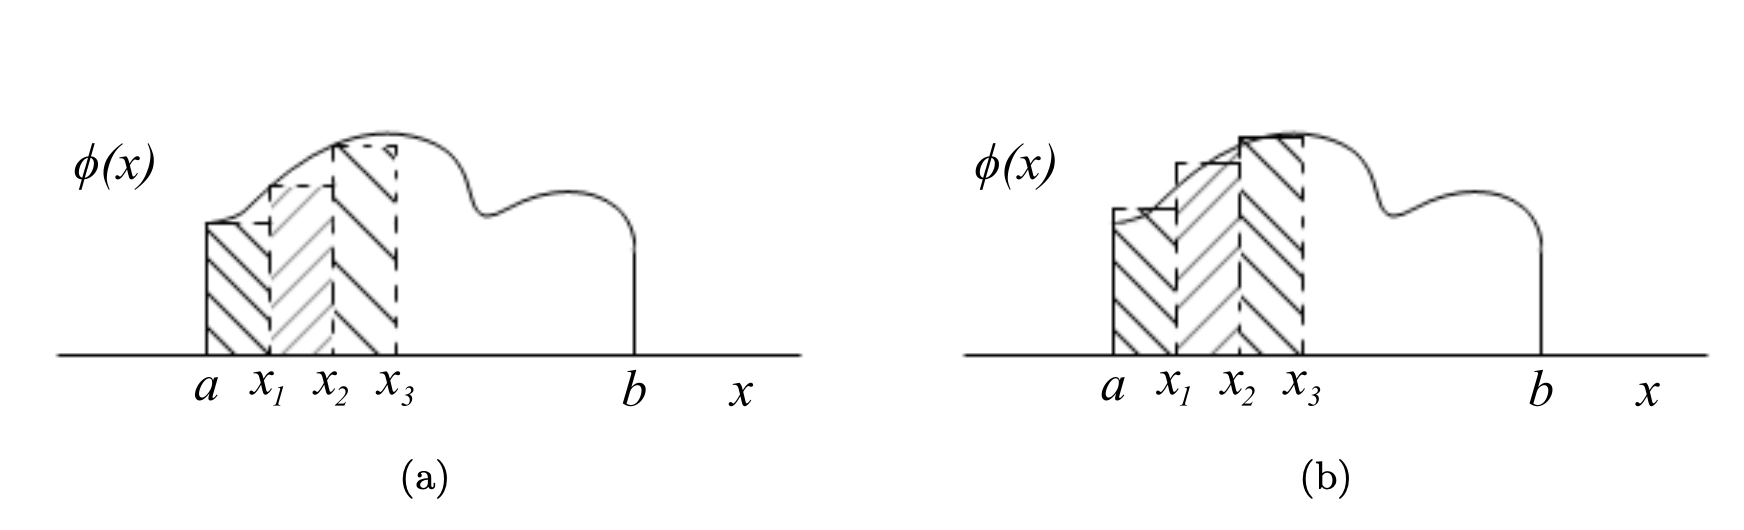
\includegraphics[scale=0.2]{Riemann and Trapezoidal.png}
    \caption{(a) Riemann approximation; (b) Trapezoidal approximation.}
    \label{}
\end{figure}\end{center}

\subsection{Multidimensional Integration}
When we want to do integral in high dimension, it will be really hard.

For $d-$dimensional integrals, the trapezoidal rule yields an approximation error $|\hat{I}_n-I|\leq \frac{C}{n^\frac{2}{d}}$ for some constant $C$. That is $n\sim O\left(\varepsilon^{-\frac{d}{2}}\right)$. $n$ needs to increase exponentially with $d$ to achieve a target approximation error $\varepsilon$. This phenomenon is known as \underline{the curse of dimensionality}.
\begin{center}\begin{figure}[htbp]
    \centering
    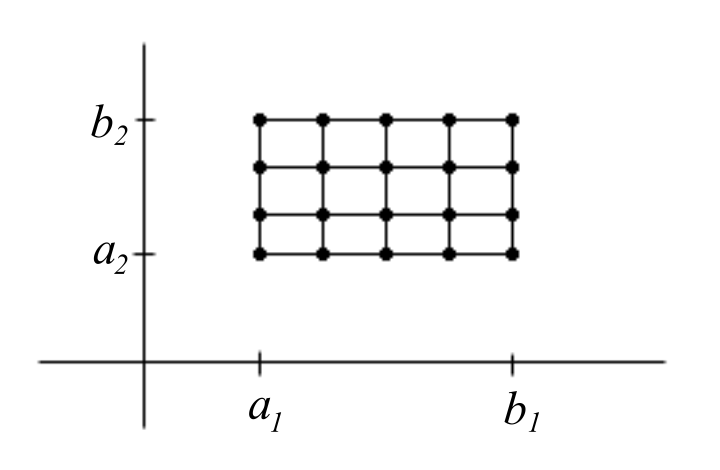
\includegraphics[scale=0.3]{two-dim int.png}
    \caption{Two-dimensional integration using regular grid.}
    \label{}
\end{figure}\end{center}




\section{Stochastic Methods (Better in High Dimension)}
\subsection{Classical Monte Carlo Integration}

Compute the expectation $$\xi=\mathbb{E}_p[h(x)]=\int_X \underbrace{p(x)h(x)}_{f(x)}dx$$

The methods described below can be used to solve the following problems: (1) General $\int_X f$; (2) Compute the probability of falling into a subset $a\subset X :P(a)=\int_a p(x)dx$, where $h(x)=\mathbf{1}_{x\in a}$

The Monte Carlo approach is as follows: Given $X_1, X_2, \cdots, X_n$ drawn i.i.d from the pdf
$p$, estimate $\xi $ by the empirical average $$\hat{\xi}_n=\frac{1}{n}\sum_{i=1}^nh(X_i)$$

$\mathbb{E}_p[\hat{\xi}_n]=\mathbb{E}_p[h(X)]=\xi$. $\hat{\xi}_n \stackrel{a.s.}{\longrightarrow}\xi$ as $n \rightarrow \infty$ by SLLW.

$Var(\hat{\xi}_n-\xi)=Var(\hat{\xi}_n)=\frac{1}{n}Var[h(x)]=O\left(\frac{1}{n}\right) \Rightarrow sd(\hat{\xi}_n)=\frac{\sqrt{Var[h(x)]}}{\sqrt{n}}$

That is $n\sim O\left(n^{-\frac{1}{2}}\right)$

The stochastic methods \textbf{outperform} when the deterministic ones for dimensions \underline{$d >4$} and are \textbf{worse} for \underline{$d<4$}.

\subsection{Importance Sampling}
Draw $X_i,i=1,...,n$ i.i.d from pdf $q$ $$\hat{\xi}_n=\frac{1}{n}\sum_{i=1}^n\frac{p(X_i)}{q(X_i)}h(X_i)$$
It is an unbiased estimator of $\xi$
\begin{equation}
    \begin{aligned}
        \mathbb{E}[\hat{\xi}_n]=\mathbb{E}_q[\frac{p(X_i)}{q(X_i)}h(X_i)]=\int_X p(x)h(x)dx=\xi
    \end{aligned}
    \nonumber
\end{equation}
$\hat{\xi}_n \stackrel{a.s.}{\longrightarrow}\xi$ as $n \rightarrow \infty$ by SLLW.

Its variance is
\begin{equation}
    \begin{aligned}
        {Var}_q(\hat{\xi}_n)&=\frac{1}{n}{Var}_q\left[\frac{p(X_i)}{q(X_i)}h(X_i)\right]\\
        &=\frac{1}{n}\left(\int_X\frac{p^2(x)}{q(x)}h^2(x)dx-\xi^2\right)
    \end{aligned}
    \nonumber
\end{equation}
The idea of importance sampling is to find a good $q$ such that $${Var}_q(\hat{\xi}_n)<{Var}_p(\hat{\xi}_n)$$

\subsection*{Error Meausre}
The \textit{relative error} of the importance-sampling estimator is defined as
$$
\delta_{\mathrm{rel}}\left(\hat{\xi}_n\right) \triangleq \frac{\sqrt{\operatorname{Var}_q\left(\hat{\xi}_n\right)}}{\xi}=\sqrt{\frac{\operatorname{Var}_q\left[\frac{p(X)}{q(X)} h(X)\right]}{\xi^2 n}} .
$$
The \textit{number} of simulations needed to achieve a relative error of $\delta$ is
$$
n_{I S}(\delta)=\frac{\operatorname{Var}_q\left[\frac{p(X)}{q(X)} h(X)\right]}{\xi^2 \delta^2} .
$$
The \textit{gain} \underline{relative to a Monte Carlo simulation} is defined as
$$
\Gamma=\frac{n_{M C}(\delta)}{n_{I S}(\delta)}=\frac{\operatorname{Var}_p[h(X)]}{\operatorname{Var}_q\left[\frac{p(X)}{q(X)} h(X)\right]}
$$

\textbf{In the example of $\xi=P(a), h(x)=\mathbf{1}_{x\in a}$:} Suppose $\xi=P(a)\approx 10^{-9}$ (small), $\hat{\xi}_n=\frac{1}{n}\sum_{i=1}^n\mathbf{1}_{X_i\in a}$. $\mathbf{1}_{X_i\in a}$ is $Bernoulli(\xi)$. We have $Var(\hat{\xi}_n)=\frac{\xi(1-\xi)}{n}$.

We can use relative error to measure $$\delta_{\mathrm{rel}}\left(\hat{\xi}_n\right)=\frac{\sqrt{Var(\hat{\xi}_n)}}{\xi}=\sqrt{\frac{1-\xi}{n\xi}}$$
and the number of simulation need to get relative error $\delta$ is $$
n_{I S}(\delta)=\frac{1-\delta} {\xi \delta^2} .
$$

\textbf{Find the optimal $q$:}
$$\min_q\int_X\frac{p^2(x)}{q(x)}h^2(x)dx-\xi^2$$
write $$\int_X\frac{p^2(x)}{q(x)}h^2(x)dx-\xi^2=\mathbb{E}_q\left[\left(\underbrace{\frac{p(x)}{q(x)}h(x)}_{Z}\right)^2\right]$$
Since $x^2$ is convex function, by Jensen's inequality
$$\mathbb{E}_q\left[\left(\underbrace{\frac{p(x)}{q(x)}h(x)}_{Z}\right)^2\right]\geq \left(\mathbb{E}_q\left[\underbrace{\frac{p(x)}{q(x)}h(x)}_{Z}\right]\right)^2$$
This equality holds if and only if $\frac{p(x)}{q(x)}h(x)=\alpha,\forall x\in X$, $\alpha$ is a constant.

Since $q$ is pdf., we can infer $$q(x)=\frac{p(x)h(x)}{\int_Xp(x)h(x)dx}$$
which is as hard as the original problem. In practice, one is content to find a “good” $q$ that assigns high probability to the important region where $p(x)h(x)$ is large. Ideally the ratio $\frac{p(x)}{q(x)}h(x)$ would be roughly constant over $X$.


\chapter{Bootstrap (not enough data)}
\underline{Problem:} analyze the performance of an estimator $\hat{\theta}_n(\vec{Y})$, $\vec{Y}=(Y_1,Y_2,...,Y_n)$ taken i.i.d. from distribution $P$. e.g. $P_{\theta}=N(0,1),\hat{\theta}_n=\frac{1}{n}\sum_{i=1}^nY_i$

Assume $\theta$ is a scalar parameter. Performance: (1) Bias $\mathbb{E}_{\theta}[\hat{\theta}_n(\vec{Y})]-\theta$; (2) Variance $\mathbb{E}_{\theta}[\hat{\theta}_n^2(\vec{Y})]-\mathbb{E}_{\theta}^2[\hat{\theta}_n(\vec{Y})]$; (3) CDF $G_{n}(t)=P(\hat{\theta}_n(\vec{Y})<t),\forall t$

\subsection*{Approach \#1 Monte-Carlo Simulations}
Generate $k$ vectors $\vec{Y}^{(i)},i=1,2,...,k$ (total $kn$ random variables)
(1) Bias $\frac{1}{k}\sum_{j=1}^k \hat{\theta}_n(\vec{Y}^{(j)})-\theta$; (2) Variance $\frac{1}{k}\sum_{j=1}^k \hat{\theta}^2_n(\vec{Y}^{(j)})-\left(\frac{1}{k}\sum_{j=1}^k \hat{\theta}_n(\vec{Y}^{(j)})\right)^2$; (3) CDF $\hat{G}_{n}(t)=\frac{1}{k}\sum_{j=1}^k \mathbf{1}_{\hat{\theta}_n(\vec{Y}^{(j)})<t},\forall t$

\subsection*{Approach \#2 Bootstrap}(When data is not enough)
Suppose we only have one data $\vec{Y}=(Y_1,...,Y_n)$

Reuse $Y_1,...Y_n$ to obtain resamples $\vec{Y}^*=(Y_1^*,...,Y_n^*)$. Do this $k$ times $\Rightarrow$ $k$ resamples ${\vec{Y^*}}^{(1)},...,{\vec{Y^*}}^{(k)}$

(1) Bias $\frac{1}{k}\sum_{j=1}^k \hat{\theta}_n(\vec{Y^*}^{(j)})-\theta$; (2) Variance $\frac{1}{k}\sum_{j=1}^k \hat{\theta}^2_n(\vec{Y^*}^{(j)})-\left(\frac{1}{k}\sum_{j=1}^k \hat{\theta}_n(\vec{Y^*}^{(j)})\right)^2$; (3) CDF $\hat{G}_{n}(t)=\frac{1}{k}\sum_{j=1}^k \mathbf{1}_{\hat{\theta}_n(\vec{Y^*}^{(j)})<t},\forall t$

\textbf{Example:} $\theta=med\{P\}$, $P$ is an unknown distribution over $\{0,1,...,9\}$. $\vec{Y}=(4,8,9,6,2)$.



\section{Residual Bootstrap}
The bootstrap principle is quite general and may also be used in problems where the data $Y_i$, $1\leq i\leq n$, \textbf{are not i.i.d}.

\subsection*{Example: Linear}
Observation $Y_i=a+b\frac{i}{n}+Z_i$, where $Z_i\sim N(0,\sigma^2)$ (i.i.d.) for $i=1,2,...,n$

Parameter $\theta=(a,b)$. Linear Least Square Estimator:
$$(\hat{a}_n,\hat{b}_n)=\argmin_{(a,b)}\sum_{i=1}^n(Y_i-a-b\frac{i}{n})^2$$
Given $\vec{Y}$, the residual (not i.i.d.)$$E_i=Y_i=\hat{a}_n-\hat{b}_n\frac{i}{n}\approx Z_i$$
Generate $k$ resamples of $\vec{E}=(E_1,E_2,...,E_n)$\\
$\Rightarrow$ obtain $\vec{E^*}^{(1)},\vec{E^*}^{(2)},...,\vec{E^*}^{(k)}$ by resampling\\
$\Rightarrow$ Compute pseudo-data ${Y_i^*}^{(j)}=\hat{a}_n+\hat{b}_n\frac{i}{n}+{E_i^*}^{(j)}$\\
$\Rightarrow$ Compute LS estimator $$\hat{\theta}_n^{(j)}=(\hat{a}_n^{(j)},\hat{b}_n^{(j)})=\argmin_{(a,b)}\sum_{i=1}^n({Y_i^*}^{(j)}-a-b\frac{i}{n})^2$$
$\Rightarrow$ Evaluate bias $$\widehat{Bias}=\frac{1}{k}\sum_{j=1}^k \hat{\theta}_n^{(j)}-\theta$$

\subsection*{Example: Nonlinear Markov Process}
Observation $Y_i=F_{\theta}(Y_{i-1})+Z_i$, where $Z_i\sim N(0,\sigma^2)$ (i.i.d.) for $i=1,2,...,n$

Parameter $\theta=(a,b)$. Linear Least Square Estimator:
$$\hat{\theta}_n(\vec{Y})=\argmin_{\theta}\sum_{i=1}^n(Y_i-F_{\theta}(Y_{i-1}))^2$$
Given $\vec{Y}$, the residual (not i.i.d.)$$E_i=Y_i=\hat{a}_n-F_{\hat{\theta}_n}(Y_{i-1})\approx Z_i$$
Generate $k$ resamples of $\vec{E}=(E_1,E_2,...,E_n)$\\
$\Rightarrow$ obtain $\vec{E^*}^{(1)},\vec{E^*}^{(2)},...,\vec{E^*}^{(k)}$ by resampling\\
$\Rightarrow$ Fix ${Y_0^*}^{(j)}=Y_0$, compute pseudo-data ${Y_i^*}^{(j)}=F_{\hat{\theta}_n}({Y^*_{i-1}}^{(j)})+{E_i^*}^{(j)}$\\
$\Rightarrow$ Compute LS estimator $$\hat{\theta}_n^{(j)}=\argmin_{(a,b)}\sum_{i=1}^n({Y_i^*}^{(j)}-F_{\hat{\theta}_n}({Y^*_{i-1}}^{(j)}))^2$$
$\Rightarrow$ Evaluate bias $$\widehat{Bias}=\frac{1}{k}\sum_{j=1}^k \hat{\theta}_n^{(j)}-\theta$$


\chapter{Particle Filtering}
Kalman filtering is used in tracking problems (dynamic models). Particle Filtering is an extension of Kalman filtering.
\section{Kalman Filtering (Linear Dynamic System)}
\begin{enumerate}
    \item Unknown state sequence $X_t\in \mathbb{R}^m,t=0,1,2,...$
    \item Observations $Y_t\in \mathbb{R}^k,t=0,1,2,...$
    \item $X_{t+1}=F_tX_t+U_t$, $F_t\in \mathbb{R}^{m\times m}, U_t\sim P_{U_t}$
    \item $Y_t=H_tX_t+V_t$, $H_t\in \mathbb{R}^{k\times m}, V_t\sim P_{V_t}$
\end{enumerate}

We want to solve two problems
\begin{enumerate}
    \item \textbf{Estimation Problem:} Evaluate Linear MMSE (LMMSE) of $X_t$ given $Y_{0:t}$. $$\hat{X}_{t|t}=WY_{0:t}+b$$
    \item \textbf{Prediction Problem:} Predict Linear MMSE (LMMSE) of $X_{t+1|t}$ given $Y_{0:t}$. (Really hard)
\end{enumerate}
We can solve closed-form solutions.

\section{Particle Filtering (Nonlinear Dynamic System)}
Particle filtering is a nonlinear form of Kalman filtering, which doesn't have closed-from solutions.

We consider a \underline{Nonlinear Dynamic System}
\begin{equation}
    \begin{aligned}
        X_{t+1}\sim q(\cdot|X_t)\\
        Y_{t}\sim r(\cdot|X_t)\\t=0,1,2,...
    \end{aligned}
    \nonumber
\end{equation}
where $q(X_{t+1}|X_t)$ is the transition probability distribution, and $r(Y_t|X_t)$ is the conditional probability distribution for the observations. Hence, $X_t$ is a Markov process and $Y_t$ follows a Hidden Markov Model (HMM).
\begin{center}\begin{figure}[htbp]
    \centering
    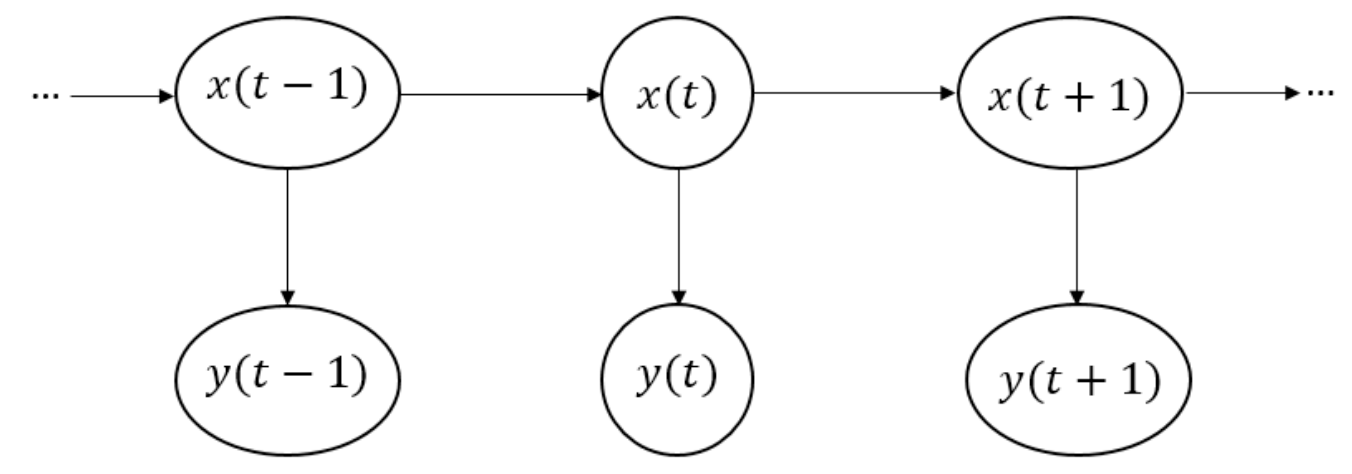
\includegraphics[scale=0.2]{HMM.png}
    \caption{Hidden Markov Model}
    \label{}
\end{figure}\end{center}
We also consider these two probelms.
\begin{enumerate}
    \item \textbf{Estimation Problem:} Evaluate $X_t$ given $Y_{0:t}$.
    \item \textbf{Prediction Problem:} Predict $X_{t+1|t}$ given $Y_{0:t}$.
\end{enumerate}

\subsection{Bayesian Recursive Filtering}
In this section we use Bayesian approach and use MMSE estimation $l(\hat{x}_t,x_t)=\|x_t-\hat{x}_t\|^2$

Estimation and prediction in conditional forms are:
\begin{equation}
    \begin{aligned}
        \hat{X}_{t|t}&=\mathbb{E}[X_{t}|Y_{0:t}]=\int_{\mathbb{R}^m}x_{t}P(X_{t}|Y_{0:t})dx_{t}\\
        \hat{X}_{t+1|t}&=\mathbb{E}[X_{t+1}|Y_{0:t}]=\int_{\mathbb{R}^m}x_{t+1}P(X_{t+1}|Y_{0:t})dx_{t+1}
    \end{aligned}
    \nonumber
\end{equation}

Apparently the posterior p.d.f cannot be evaluated due to the curse of dimensionality as $t$ increases. However, they can in principle be evaluated \textit{recursively} using the following two-step procedure.

\begin{enumerate}[\textbf{Step}]
    \item \textbf{ 1: Prediction.} $P(X_{t+1}|Y_{0:t})$ can be expressed in term of $P(X_t|Y_{0:t})$:
    \begin{equation}
        \begin{aligned}
            P(X_{t+1}|Y_{0:t})&=\int_{\mathbb{R}^m}P(X_{t+1},X_t|Y_{0:t})dx_t\\
            &=\int_{\mathbb{R}^m}P(X_{t+1}|X_t, Y_{0:t})P(X_t|Y_{0:t})dx_t\\
            &=\int_{\mathbb{R}^m}q(X_{t+1}|X_t)P(X_t|Y_{0:t})dx_t\\
        \end{aligned}
        \nonumber
    \end{equation}
    \item \textbf{ 2: Update.} We can also express $P(X_t|Y_{0:t})$ in terms of $P(X_t|Y_{0:t-1})$
    \begin{equation}
        \begin{aligned}
            P(X_{t}|Y_{0:t})&=P(X_t|Y_{t},Y_{0:t-1})\\
            &=\frac{P(Y_t|X_t,Y_{0:t-1})P(X_t|Y_{0:t-1})}{P(Y_t|Y_{0:t-1})}\\
            &=\frac{r(Y_t|X_t)P(X_t|Y_{0:t-1})}{\int_{\mathbb{R}^m}r(Y_t|X_t)P(X_t|Y_{0:t-1})dx_t}
        \end{aligned}
        \nonumber
    \end{equation}
\end{enumerate}

\subsection{Particle Filter (bootstrap filter)}
Suppose we have $n$ i.i.d. samples of $X_t$ drawn from $p(x_t|Y_{0:t})$: $X_t(1),X_t(2),...,X_t(n)$.
\begin{equation}
    \begin{aligned}
        X_{t}(i)\sim p(\cdot|Y_{0:t}),1\leq i\leq n
    \end{aligned}
    \tag{\text{Sample 1}}
\end{equation}

We can use above recursive filtering method to generate estimation of $X_{t+1}$.
\begin{enumerate}[\textbf{Step}]
    \item \textbf{ 1: Prediction.} Using the transition probability $q(\cdot|X_t(i)),1\leq i\leq n$ to generate $n$ independent random variables
    \begin{equation}
        \begin{aligned}
            X^*_{t+1}(i)\sim q(\cdot|X_t(i)),\ 1\leq i\leq n
        \end{aligned}
        \tag{\text{Sample 2}}
    \end{equation}
    \item \textbf{ 2: Update.} Upon \textbf{receiving a new measurement $y_{t+1}$}, evaluate the \textit{importance weights} (nonnegative and summing to $1$)
    \begin{equation}
        \begin{aligned}
            w_i=\frac{r(y_{t+1}|X_{t+1}^*(i))}{\sum_{j=1}^n r(y_{t+1}|X_{t+1}^*(j))},\ 1\leq i\leq n
        \end{aligned}
        \nonumber
    \end{equation}
    Then we resample $n$ times from the set $\{X_{t+1}^*(i)\}_{i=1}^n$ with respective probabilities $\{w_i\}_{i=1}^n$, obtaining i.i.d samples $\{X_{t+1}(j)\}_{j=1}^n$ with probabilities
    \begin{equation}
        \begin{aligned}
            Pr[X_{t+1}(j)=X_{t+1}^*(i)]=w_i,\ 1\leq i,j\leq n
        \end{aligned}
        \tag{\text{Sample 3}}
    \end{equation}
\end{enumerate}
By the \textbf{weighted bootstrap theorem}, as $n \rightarrow \infty$, the distribution of the
resampled $\{X_{t+1}(j)\}_{j=1}^n$ converges to the desired posterior.


Potential issues: 1. $n$ is not large enough. 2. Sample impoverishment





\chapter{EM Algorithm}

The ML estimator: $\hat{\theta}_{ML}=\argmax_{\theta\in S}\ln p_\theta(y)$. Numerical evaluation of maximum-likelihood (ML) estimates is often difficult. The likelihood function may have multiple extreme and the parameter $\theta$ may be multidimensional, all of which are problematic for any numerical algorithm.

\subsection*{Maximum-Likelihood (ML) Estimation}
Given a vector $\vec{y}$, find the $\theta$ that maximizes $p_\theta(\vec{y})=\prod_{i=1}^n P(y_i|\theta)$
$$\hat{\theta}_{ML}=\argmax_{\theta\in S}\ln p_\theta(\vec{y})=\argmax_{\theta\in S}\sum_{i=1}^n \ln P(y_i|\theta)$$
Solving the closed-form solution is quite hard sometimes, so we may use EM algorithm.

\section{General Structure of the EM Algorithm}

\subsection*{What we want to estimate:}
$\theta\in S$ is an unknown parameter that we want to estimate.
\subsection*{What we know:}
To help us solve the solution, we construct an unobservable vector $\vec{z}$ corresponding to $\vec{y}$.
\begin{enumerate}
    \item There is a complete data space $Z$ and an incomplete data space $Y$.
    \item The reality is $z\in Z$, which has p.d.f $P(z|\theta)$. ($\ln P(z|\theta)$'s derivative should be constructed to be easy.)
    \item \textbf{Instead of observing the $z$ directly, we can observe $y=h(z)\in Y$ which has p.d.f $P(y|\theta)$.}
    \item $h(z)=y$ is a many-to-one mapping. $$P(y,z|\theta)=P(z|\theta),\quad \forall z\in h^{-1}(y)$$
    \item We can infer that the relationship between $P(z|\theta)$ and $P(y|\theta)$ is
    \begin{equation}
        \begin{aligned}
            P(z|\theta)&=P(z|y,\theta)P(y|\theta),\quad \forall z\in h^{-1}(y)\\
            P(y|\theta)&=\sum_{z\in h^{-1}(y)}P(z|\theta),\quad \forall y
        \end{aligned}
        \nonumber
    \end{equation}
    \item For any function $f$, $\mathbb{E}_z[f(z)|y]$ depends on the p.d.f.
    \begin{equation}
        \begin{aligned}
            \mathbb{E}_{z|\theta}[f(z)|y]=\sum_{z\in h^{-1}(y)}P(z|y,\theta)f(z)
        \end{aligned}
        \nonumber
    \end{equation}
\end{enumerate}
\begin{center}\begin{figure}[htbp]
    \centering
    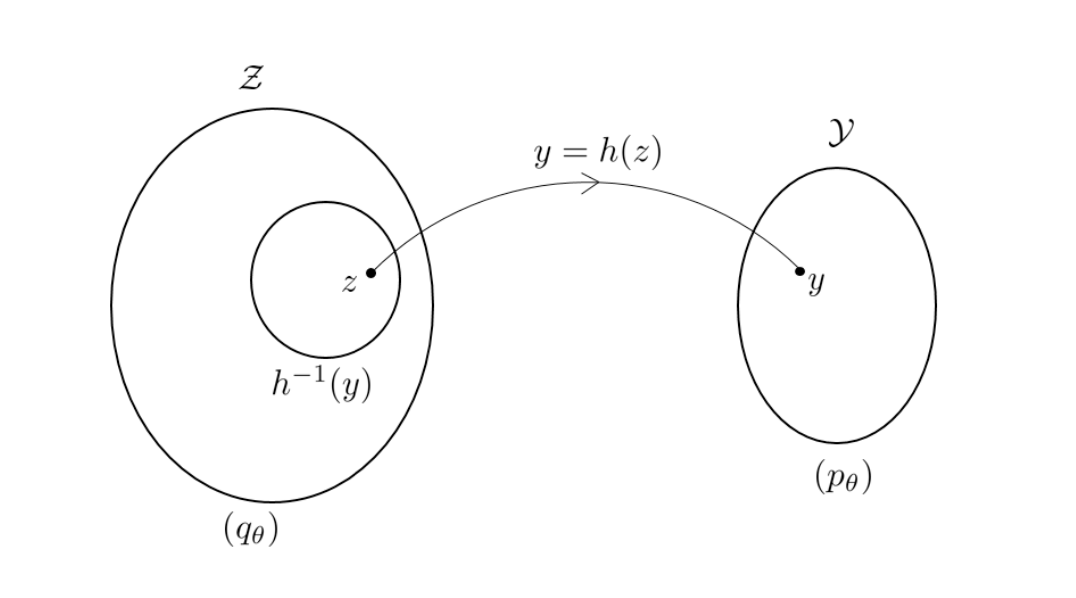
\includegraphics[scale=0.2]{EM1.png}
    \caption{Complete and incomplete data spaces $Z$ and $Y$.}
    \label{}
\end{figure}\end{center}

%The incomplete-data and complete-data loglikelihood functions are respectively denoted by
%\begin{equation}
%    \begin{aligned}
        %l_{id}(\theta)\triangleq \ln p_\theta(y);\ l_{cd}(\theta)\triangleq \ln q_\theta(z)
%    \end{aligned}
%    \nonumber
%\end{equation}
\subsection*{EM Algorithm}
Instead of computing the $P(\vec{y}|\theta)$ directly, we use the relationship $h(z)=y$ and $P(\vec{z}|\theta)$ to estimate $\theta$.

Suppose we have a prior belief of the relationship between $y$ and $z$: $P(z|y,\theta^{(k)})$. Given $\vec{y}$, since maximizing $\ln P(\vec{y}|\theta)$ is hard, we maximize the expected value of $\ln P(\vec{z}|\theta)|\vec{y}$ under the prior belief (i.e., finding the $\theta$ that can properly represent the relationship between $\vec{y}$ and $\vec{z}$), that is
\begin{equation}
    \begin{aligned}
        \theta&=\argmax_\theta \mathbb{E}_{z|y,\theta^{(k)}} [\ln P(\vec{z}|\theta)|\vec{y}]\\
        &=\argmax_\theta\sum_{i=1}^n \sum_{z_i\in h^{-1}(y_i)}P(z_i|y_i,\theta^{(k)})\ln P(z_i|\theta)
    \end{aligned}
    \nonumber
\end{equation}

EM algorithm alternates between Expectation (E) and Maximization (M) steps:
\begin{enumerate}
    \item Initialize $\hat{\theta}^{(0)}$
    \item For $k=0,1,2,...$\\
    \textbf{Expectation (E)-Step:}
        Compute
        \begin{equation}
            \begin{aligned}
                Q(\theta|\hat{\theta}^{(k)})
                &=\mathbb{E}_{z|y,\hat{\theta}^{(k)}}[\ln P(\vec{z}|\theta)|\vec{y}]\\
                &=\sum_{i=1}^n \sum_{z_i\in h^{-1}(y_i)}P(z_i|y_i,\theta^{(k)})\ln P(z_i|\theta)
            \end{aligned}
            \nonumber
        \end{equation}
    \textbf{Maximization (M)-Step} $$\hat{\theta}^{(k+1)}=\argmax_{\theta\in S}Q(\theta|\hat{\theta}^{(k)})$$
\end{enumerate}

\begin{definition}
    $\theta^*$ is a stable point of the EM algorithm if $\exists$ subsequence that converges to $\theta^*$.

    e.g. $1,3,\frac{1}{2},3,\frac{1}{3},3,...\frac{1}{n},3,...$
\end{definition}

\section{Example 1: Variance Estimation}
Observation $Y=S+N$, $S\sim \mathcal{N}(0,\theta)$ is independent of $N\sim \mathcal{N}(0,\theta)$ $\Rightarrow$ $Y\sim \mathcal{N}(0,\theta+1)$. $p_\theta(y)=\frac{1}{\sqrt{2\pi(\theta+1)}}e^{-\frac{y^2}{2(\theta+1)}}$. We want to estimate $\theta$.
\subsection{Maximum-Likelihood (ML) Estimation}
\begin{equation}
    \begin{aligned}
        \ln p_\theta(y)=-\frac{1}{2}\ln (2\pi)-\frac{1}{2}\ln(\theta+1)-\frac{y^2}{2(\theta+1)}
    \end{aligned}
    \nonumber
\end{equation}
take derivation of $\theta$ to be equal to $0$
\begin{equation}
    \begin{aligned}
        -\frac{1}{2(\theta+1)}+\frac{y^2}{2(\theta+1)^2}=0
    \end{aligned}
    \nonumber
\end{equation}
We can get $$\hat{\theta}=y^2-1$$
Then, $$\hat{\theta}_{ML}=\left\{\begin{matrix}
    0,&y^2\leq 1\\
    y^2-1,&y^2>1
\end{matrix}\right.$$

\subsection{EM Algorithm}
Let $Z=(S,N)$, $y=h(z)=s+n$.
\begin{equation}
    \begin{aligned}
        q_\theta(z)=q_\theta(s,n)=\frac{1}{\sqrt{2\pi\theta}}e^{-\frac{s^2}{2\theta}}\frac{1}{\sqrt{2\pi}}e^{-\frac{n^2}{2}}
    \end{aligned}
    \nonumber
\end{equation}
Then $$\ln q_\theta(z)=\ln \frac{1}{\sqrt{2\pi}}e^{-\frac{n^2}{2}}-\frac{1}{2}\ln (2\pi)-\frac{1}{2}\ln(\theta)-\frac{s^2}{2\theta}$$
\textbf{E-Step:}
        Compute
        \begin{equation}
            \begin{aligned}
                Q(\theta|\hat{\theta}^{(k)})
                &=\mathbb{E}_{z|\hat{\theta}^{(k)}}[\ln q_\theta(z)|Y=y]\\
                &=\sum_{z\in h^{-1}(y)}q_{\hat{\theta}^{(k)}}(z)\ln q_\theta(z)\\
                &=\ln \frac{1}{\sqrt{2\pi}}e^{-\frac{n^2}{2}}-\frac{1}{2}\ln (2\pi)-\frac{1}{2}\ln(\theta)-\frac{\mathbb{E}_{z|\hat{\theta}^{(k)}}(s^2)}{2\theta}
            \end{aligned}
            \nonumber
        \end{equation}
\textbf{M-Step}
\begin{equation}
    \begin{aligned}
        \hat{\theta}^{(k+1)}&=\argmax_{\theta\in S}Q(\theta|\hat{\theta}^{(k)})\\
        0&=-\frac{1}{2\hat{\theta}^{(k+1)}}+\frac{\mathbb{E}_{z|\hat{\theta}^{(k)}}(s^2)}{2(\hat{\theta}^{(k+1)})^2}\\
        \hat{\theta}^{(k+1)}&=\mathbb{E}_{z|\hat{\theta}^{(k)}}(s^2)=\frac{\hat{\theta}^{(k)}}{\hat{\theta}^{(k)}+1}\left(\frac{\hat{\theta}^{(k)}}{\hat{\theta}^{(k)}+1}y^2+1\right)
    \end{aligned}
    \nonumber
\end{equation}
Then we can solve the stable point
\begin{equation}
    \begin{aligned}
        \hat{\theta}^{*}=\frac{\hat{\theta}^{*}}{\hat{\theta}^{*}+1}\left(\frac{\hat{\theta}^{*}}{\hat{\theta}^{*}+1}y^2+1\right)\\
        \Rightarrow \hat{\theta}^{*}=0, \hat{\theta}^{*}=y^2-1
    \end{aligned}
    \nonumber
\end{equation}
According to the relation between $\hat{\theta}^{(k)}$ and $\hat{\theta}^{(k+1)}$, we can infer
$$\hat{\theta}^*=\left\{\begin{matrix}
    0,&y^2\leq 1\\
    y^2-1,&y^2>1
\end{matrix}\right.$$







\section{Example 2: Estimation of Gaussian Mixtures}
Assume the data $\vec{Y}=\left\{Y_i, 1 \leq i \leq n\right\} \in \mathbb{R}^n$, are drawn iid from a pdf $p_\theta(y)$ which is the mixture of $m$ univariate Gaussians with respective probabilities $\pi(j)$, means $\mu_j$, and variances $\sigma_j^2$, for $1 \leq j \leq m$ :
$$p_\theta(y|j)=\phi\left(y ; \mu_j, \sigma_j^2\right)$$
$$
p_\theta(y)=\sum_{j=1}^m \pi(j) \phi\left(y ; \mu_j, \sigma_j^2\right), \quad y \in \mathbb{R}
$$
where
$$\phi\left(y ; \mu, \sigma^2\right) \triangleq \frac{1}{\sqrt{2 \pi \sigma^2}} \exp \left\{-\frac{(y-\mu)^2}{2 \sigma^2}\right\}$$
denotes the Gaussian pdf with mean $\mu$ and variance $\sigma^2$.
\subsection{Unknown Means: ML estimation is hard}
We initially assume that $\{\pi(j)\}$ and $\left\{\sigma_j^2\right\}$ are given and that we only need to estimate the means $\left\{\mu_j\right\}$. Thus, $\theta=\mu \in \mathbb{R}^m$.

Unfortunately the ML estimator cannot be derived in closed form. Indeed, the loglikelihood function for $\theta$ is
$$
\ln \prod_{i=1}^n p_\theta(y_i)=\sum_{i=1}^n \ln p_\theta\left(y_i\right)=\sum_{i=1}^n \ln \sum_{j=1}^m \pi(j) \phi\left(y_i ; \mu_j, \sigma_j^2\right)
$$
and maximizing it is a $m$-dimensional, nonconcave maximization problem.

Taking the derivative of $\mu_j, j=1,...,m$,
\begin{equation}
    \begin{aligned}
        0&=\frac{1}{\sigma^2_j}\sum_{i=1}^n(y_i-\mu_j)\frac{\pi(j)\phi(y_i ; \mu_j, \sigma_j^2)}{\sum_{j=1}^m\pi(j)\phi(y_i ; \mu_j, \sigma_j^2)}\\
        &=\frac{1}{\sigma^2_j}\sum_{i=1}^n(y_i-\mu_j)\pi_\theta(j|y_i)
    \end{aligned}
    \nonumber
\end{equation}
where $\pi_\theta(j|y_i)\triangleq \frac{\pi(j)\phi(y_i ; \mu_j, \sigma_j^2)}{\sum_{j=1}^m\pi(j)\phi(y_i ; \mu_j, \sigma_j^2)}$.
The system may have multiple solutions corresponding to local maxima or even local minima or saddle points of the likelihood function.

\subsection{Unknown Means: EM Algorithm}

There is a complete data $Z_i=(J_i,Y_i),=1,...,n$, where $J_i$ is the random label that was drawn to produce $Y_i$. $z=\{j_i,y_i\}_{i=1}^n$ is the sample.
\begin{equation}
    \begin{aligned}
        q_\theta(z)&=\prod_{i=1}^n\left(\pi(j_i)p_\theta(y_i|j_i)\right)
    \end{aligned}
    \nonumber
\end{equation}
$$\ln q_{\theta}(z)=\sum_{i=1}^n[\ln \pi(j_i)+\ln p_{\theta}(y_i|j_i)]$$

Initialize $\hat{\theta}^{(0)}$

Iteration:
\begin{equation}
    \begin{aligned}
        Q(\theta|\hat{\theta}^{(k)})
        &=\sum_{i=1}^n\mathbb{E}_{\hat{\theta}^{(k)}}[\ln \pi(j_i)+\ln p_{\theta}(y_i|j_i)|Y_i=y_i]\\
        &=\sum_{i=1}^n\sum_{j=1}^m\pi_{\hat{\theta}^{(k)}}(j|y_i)[\ln \pi(j)+\ln p_{\theta}(y_i|j)]\\
        &=cst-\sum_{i=1}^n\sum_{j=1}^m\pi_{\hat{\theta}^{(k)}}(j|y_i)\frac{(y_i-\mu_j)^2}{2\sigma_j^2}\\
        &=cst-\sum_{i=1}^n\sum_{j=1}^m\frac{\pi(j)\phi(y_i ; \hat{\mu}_j^{(k)}, \sigma_j^2)}{\sum_{j=1}^m\pi(j)\phi(y_i ; \hat{\mu}_j^{(k)}, \sigma_j^2)}\frac{(y_i-\mu_j)^2}{2\sigma_j^2}
    \end{aligned}
    \nonumber
\end{equation}
where $\ln p_{\theta}(y_i|j)=-\frac{1}{2}\ln(2\pi\sigma_j^2)-\frac{(y_i-\mu_j)^2}{2\sigma_j^2}$.

Take derivative of $\mu_j$,
\begin{equation}
    \begin{aligned}
        0&=\frac{\partial Q(\theta|\hat{\theta}^{(k)})}{\partial \mu_j}=\sum_{i=1}^n\pi_{\hat{\theta}^{(k)}}(j|y_i)\frac{(y_i-\mu_j)}{\sigma_j^2}\\
        \hat{\mu}_j^{(k+1)}&=\frac{\sum_{i=1}^n\pi_{\hat{\theta}^{(k)}}(j|y_i)y_i}{\sum_{i=1}^n\pi_{\hat{\theta}^{(k)}}(j|y_i)}
    \end{aligned}
    \nonumber
\end{equation}

Recall the $\hat{\theta}_{ML}$
\begin{equation}
    \begin{aligned}
        \hat{\theta}_{ML,j}=\frac{\sum_{i=1}^n\pi_{\hat{\theta}_{ML}}(j|y_i)y_i}{\sum_{i=1}^n\pi_{\hat{\theta}_{ML}}(j|y_i)}
    \end{aligned}
    \nonumber
\end{equation}
$\hat{\theta}_{ML}$ is the stable point. (if exist)

\subsection{Unknown Mixture Probabilities, Means and Variances}
\textbf{ML Estimation:}

If $\theta \triangleq\left\{\pi(j), \mu_j, \sigma_j^2, 1 \leq j \leq m\right\}$ is unknown, the ML estimator $\hat{\theta}_{\mathrm{ML}}$ satisfies the following nonlinear system of equations:
$$
\begin{aligned}
\hat{\mu}_{\mathrm{ML}, j} &=\frac{\sum_{i=1}^n y_i \pi_{\hat{\theta}^{(k)}}\left(j \mid y_i\right)}{\sum_{i=1}^n \pi_{\hat{\theta}^{(k)}}\left(j \mid y_i\right)} \\
\hat{\sigma}_{\mathrm{ML}, j}^2 &=\frac{\sum_{i=1}^n\left(y_i-\hat{\mu}_{\mathrm{ML}, j}\right)^2 \pi_{\hat{\theta}^{(k)}}\left(j \mid y_i\right)}{\sum_{i=1}^n \pi_{\hat{\theta}(k)}\left(j \mid y_i\right)} \\
\hat{\pi}_{\mathrm{ML}}(j) &=\frac{1}{n} \sum_{i=1}^n \pi_{\hat{\theta}^{(k)}}\left(j \mid y_i\right) \quad 1 \leq j \leq m
\end{aligned}
$$
where
$$
\pi_\theta\left(j \mid y_i\right)=\frac{\pi(j) \phi\left(y_i ; \mu_j, \sigma_j^2\right)}{\sum_{j=1}^m \pi(j) \phi\left(y_i ; \mu_j, \sigma_j^2\right)}, \quad 1 \leq j \leq m
$$
\textbf{E-step:}
\begin{equation}
    \begin{aligned}
        Q(\theta|\hat{\theta}^{(k)})
        &=cst-\sum_{i=1}^n\sum_{j=1}^m\pi_{\hat{\theta}^{(k)}}(j|y_i)\frac{(y_i-\mu_j)^2}{2\sigma_j^2}\\
        &=cst-\sum_{i=1}^n\sum_{j=1}^m\frac{\hat{\pi}^{(k)}(j)\phi(y_i ; \hat{\mu}_j^{(k)}, \hat{\sigma_j^2}^{(k)})}{\sum_{j=1}^m\hat{\pi}^{(k)}(j)\phi(y_i ; \hat{\mu}_j^{(k)}, \hat{\sigma_j^2}^{(k)})}\frac{(y_i-\mu_j)^2}{2\sigma_j^2}
    \end{aligned}
    \nonumber
\end{equation}
\textbf{M-Step:}
\begin{equation}
    \begin{aligned}
        \hat{\mu}_j^{(k+1)} &=\frac{\sum_{i=1}^n y_i \pi_{\hat{\theta}^{(k)}}\left(j \mid y_i\right)}{\sum_{i=1}^n \pi_{\hat{\theta}(k)}\left(j \mid y_i\right)} \\
        \left(\hat{\sigma}_j^2\right)^{(k+1)} &=\frac{\sum_{i=1}^n\left(y_i-\hat{\mu}_j^{(k+1)}\right)^2 \pi_{\hat{\theta}^{(k)}}\left(j \mid y_i\right)}{\sum_{i=1}^n \pi_{\hat{\theta}^{(k)}}\left(j \mid y_i\right)} \\
        \hat{\pi}^{(k+1)}(j) &=\frac{1}{n} \sum_{i=1}^n \pi_{\hat{\theta}^{(k)}}\left(j \mid y_i\right), \quad 1 \leq j \leq m .
    \end{aligned}
    \nonumber
\end{equation}


\section{Convergence of EM Algorithm}
\begin{theorem}
    The likelihood sequence $p_{\hat{\theta}^{(k)}}(y)$, $k = 0, 1, 2, ...$ is nondecreasing.
\end{theorem}
\begin{proof}
    Assume for notational simplicity that the random variables $Y$ and $Z$ are discrete. Hence, their joint distribution is given by
    \begin{equation}
        \begin{aligned}
            P_\theta(y,z)&=q_\theta(z)p_\theta(y|z)=q_\theta(z)\mathbf{1}_{\{y=h(z)\}}\\
            &=p_\theta(y)q_\theta(z|y)
        \end{aligned}
        \nonumber
    \end{equation}
    Given $y$, the following identity holds for all $z \in h^{-1}(y)$:
    \begin{equation}
        \begin{aligned}
            p_\theta(y)&=\frac{q_\theta(z)}{q_\theta(z|y)}
        \end{aligned}
        \nonumber
    \end{equation}
    Taking the logarithm,
    \begin{equation}
        \begin{aligned}
            \ln p_\theta(y)&= \ln q_\theta(z)-\ln q_\theta(z|y),\ \forall z\in h^{-1}(y)
        \end{aligned}
        \nonumber
    \end{equation}
    Taking the conditional expectation with respect to $q_{\hat{\theta}}(z|y)$,
    \begin{equation}
        \begin{aligned}
            \ln p_\theta(y)&= \sum_{z\in h^{-1}(y)}q_{\hat{\theta}}(z|y)\ln q_\theta(z)-\sum_{z\in h^{-1}(y)}q_{\hat{\theta}}(z|y)\ln q_\theta(z|y)
        \end{aligned}
        \tag{1}
    \end{equation}
    \textbf{Expectation (E)-Step:}
        Compute
        \begin{equation}
            \begin{aligned}
                Q(\theta|\hat{\theta}^{(k)})
                &=\sum_{z\in h^{-1}(y)}q_{\hat{\theta}^{(k)}}(z|y)\ln q_\theta(z)
            \end{aligned}
            \nonumber
        \end{equation}
    \textbf{Maximization (M)-Step} $$\hat{\theta}^{(k+1)}=\argmax_{\theta\in S}Q(\theta|\hat{\theta}^{(k)})$$

    According to $(1)$,
    \begin{equation}
        \begin{aligned}
            \ln p_\theta (y)&=Q(\theta|\hat{\theta}^{(k)})-H(q_{\hat{\theta}^{(k)}},q_\theta)\\
            \ln p_{\hat{\theta}^{(k+1)}} (y)-\ln p_{\hat{\theta}^{(k)}} (y)&=(Q(\hat{\theta}^{(k+1)}|\hat{\theta}^{(k)})-Q(\hat{\theta}^{(k)}|\hat{\theta}^{(k)}))-(H(q_{\hat{\theta}^{(k)}},q_{\hat{\theta}^{(k+1)}})-H(q_{\hat{\theta}^{(k)}},q_{\hat{\theta}^{(k)}}))
        \end{aligned}
        \nonumber
    \end{equation}
    Since $\hat{\theta}^{(k+1)}=\argmax_{\theta\in S}Q(\theta|\hat{\theta}^{(k)})$, $Q(\hat{\theta}^{(k+1)}|\hat{\theta}^{(k)})-Q(\hat{\theta}^{(k)}|\hat{\theta}^{(k)})\geq 0$.
    \begin{equation}
        \begin{aligned}
            H(q_{\hat{\theta}^{(k)}},q_{\hat{\theta}^{(k+1)}})-H(q_{\hat{\theta}^{(k)}},q_{\hat{\theta}^{(k)}})=D(q_{\hat{\theta}^{(k)}}\| q_{\hat{\theta}^{(k+1)}})\geq 0
        \end{aligned}
        \nonumber
    \end{equation}
    Hence, we can conclude $\ln p_{\hat{\theta}^{(k+1)}} (y)-\ln p_{\hat{\theta}^{(k)}} (y)\geq 0$. Then $p_{\hat{\theta}^{(k)}}$ should be nondecreasing in $k$.
\end{proof}

\begin{corollary}
    Assume that $S$ is a closed, bounded subset of Euclidean space, the functions $Q(\theta|\theta')$ and $H(\theta|\theta')$ are continuously differentiable, and the loglikelihood function $\ln p_{\hat{\theta}^{(k)}}$ is differentiable and bounded. Then the sequence $\ln p_{\hat{\theta}^{(k)}}$ converges, and any limit point $\theta^*\in \text{interior}(S)$ of the EM sequence is a solution of the likelihood equation $\nabla \ln p_{\theta}=0$.
\end{corollary}


\section{EM As an Alternating Maximization Algorithm}
Define an \textit{auxiliary cost function} $L(q,\theta)$.

Incomplete data $Y$; Complete data $Z$. Still $h(z): Z \rightarrow Y$.

$\mathcal{Q}_y=\{q: q(z)=0, \forall z\in h^{-1}(y)\}$

\underline{EM updates}
\begin{enumerate}
    \item E-Step:
\end{enumerate}













\chapter{Hidden Markov model (HMM)}
A Markov chain ${X_t}_{t\geq 1}$ is observed as $\{Y_t\}_{t\geq 1}$. The state sets are finite sets $S_x, S_y$. Suppose the initial state distribution is $\pi$. The \textit{transition probability matrix} of the MC is
\begin{equation}
    \begin{aligned}
        A(i,j)=P(X_{t+1}=j|X_{t}=i),\ i,j\in S_x
    \end{aligned}
    \nonumber
\end{equation}
and the \textit{emission probability matrix} is
\begin{equation}
    \begin{aligned}
        B(i,j)=P(Y_t=j|X_t=i),\ i\in S_x, j\in S_y
    \end{aligned}
    \nonumber
\end{equation}
\begin{center}\begin{figure}[htbp]
    \centering
    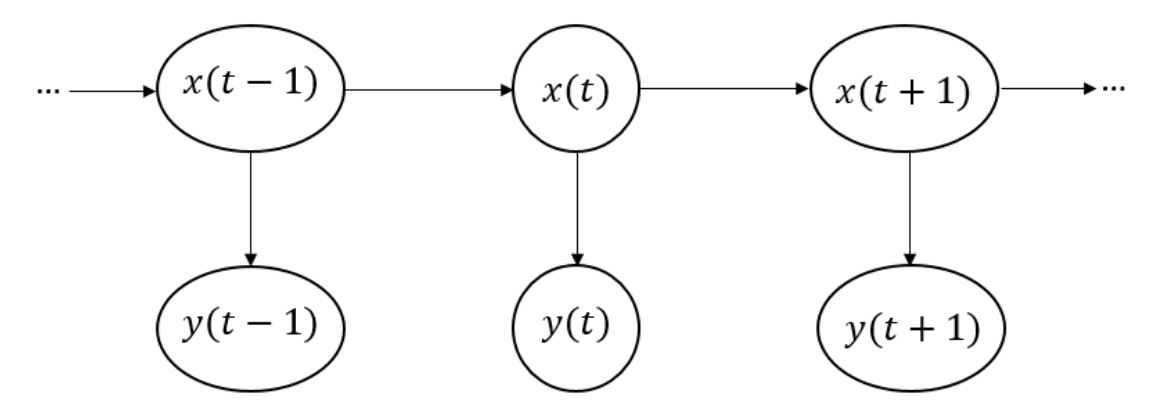
\includegraphics[scale=0.15]{HDM.png}
    \caption{Hidden Markov Model (HMM)}
    \label{}
\end{figure}\end{center}

Relative problems include
\begin{enumerate}[\textbf{Problem} 1:]
    \item Estimate $X_t$ given $Y_{1:t}$ (Using MAP or MMSE criterion: particle filtering)
    \item Estimate $X_{t+1}$ given $Y_{1:t}$ (Using MAP or MMSE prediction: particle filtering)
    \item Estimate $X_{1:t}$ given $Y_{1:t}$ (MAP, MMSE)
    \item Estimate the HMM parameters $\theta=(\pi,A,B)$ given $Y_{1:t}$ (learning)
\end{enumerate}

\section{Viterbi Algorithm: (MAP) estimate $X_{1:t}$ given $Y_{1:t}$}
\subsection{MAP estimation problem}
The MAP estimation problem arises in a variety of applications, and Viterbi derived a remarkable algorithm for solving it exactly. The probability of state $\vec{x}\in S_x^n$ is given by
\begin{equation}
    \begin{aligned}
        P(\vec{x})=\pi(x_1)\prod_{t=1}^{n-1}A(x_t,x_{t+1})
    \end{aligned}
    \nonumber
\end{equation}
and the conditional probability of the observed sequence $\vec{y}$ given the state sequence $\vec{x}$ is
\begin{equation}
    \begin{aligned}
        P(\vec{y}|\vec{x})=\prod_{t=1}^n B(x_t,y_t)
    \end{aligned}
    \nonumber
\end{equation}
Hence, the joint probability of $\vec{x}$ and $\vec{y}$ is
\begin{equation}
    \begin{aligned}
        P(\vec{x},\vec{y})=P(\vec{x})P(\vec{y}|\vec{x})=\pi(x_1)\prod_{t=1}^{n-1}A(x_t,x_{t+1})\prod_{t=1}^n B(x_t,y_t)
    \end{aligned}
    \nonumber
\end{equation}
Then the MAP estimation problem is
\begin{equation}
    \begin{aligned}
        \vec{x}^*&=\argmax_{\vec{x}}P(\vec{x}|\vec{y})=\argmax_{\vec{x}}\frac{P(\vec{x},\vec{y})}{P(\vec{y})}=\argmax_{\vec{x}}P(\vec{x},\vec{y})\\
        &=\argmax_{\vec{x}}\ \pi(x_1)\prod_{t=1}^{n-1}A(x_t,x_{t+1})\prod_{t=1}^n B(x_t,y_t)\\
        &=\argmax_{\vec{x}}\ \ln\pi(x_1)+\sum_{t=1}^{n-1}\ln A(x_t,x_{t+1})+\sum_{t=1}^n\ln B(x_t,y_t)
    \end{aligned}
    \nonumber
\end{equation}

\subsection{Viterbi Algorithm}
Let $f(x_1)=\ln\pi(x_1)+\ln B(x_1,y_1)$, $g_t(x_t,x_{t+1})=\ln A(x_t,x_{t+1})+\ln B(x_{t+1},y_{t+1})$. Then the estimation problem is written in the form
\begin{equation}
    \begin{aligned}
        \vec{x}^*=\argmax_{\vec{x}}\ \left[\varepsilon (\vec{x})=f(x_1)+\sum_{u=1}^{n-1}g_u(x_u,x_{u+1})\right]
    \end{aligned}
    \nonumber
\end{equation}
Let $V(1,x)=f(x)$ and
\begin{equation}
    \begin{aligned}
        V(t,x_t=x)\triangleq \max_{x_1,x_2,...,x_{t-1}}\left[\varepsilon([x_1,...,x_t])=f(x_1)+\sum_{u=1}^{t-1}g_u(x_u,x_{u+1})\right]
    \end{aligned}
    \nonumber
\end{equation}
\begin{equation}
    \begin{aligned}
        V(t,x_t=x)=\max_{x'} \left[V(t-1,x_{t-1}=x')+g_{t-1}(x',x)\right],\ t\geq 2
    \end{aligned}
    \nonumber
\end{equation}
Then, when $t=n$ we have
\begin{equation}
    \begin{aligned}
        \max_{\vec{x}}\varepsilon(\vec{x})=\max_{x} V(n,x_n=x)
    \end{aligned}
    \nonumber
\end{equation}

The complexity of the algorithm is $O(n|S_x|)$ storage and $O(n|S_x|^2)$ computation.

\begin{center}\begin{figure}[htbp]
    \centering
    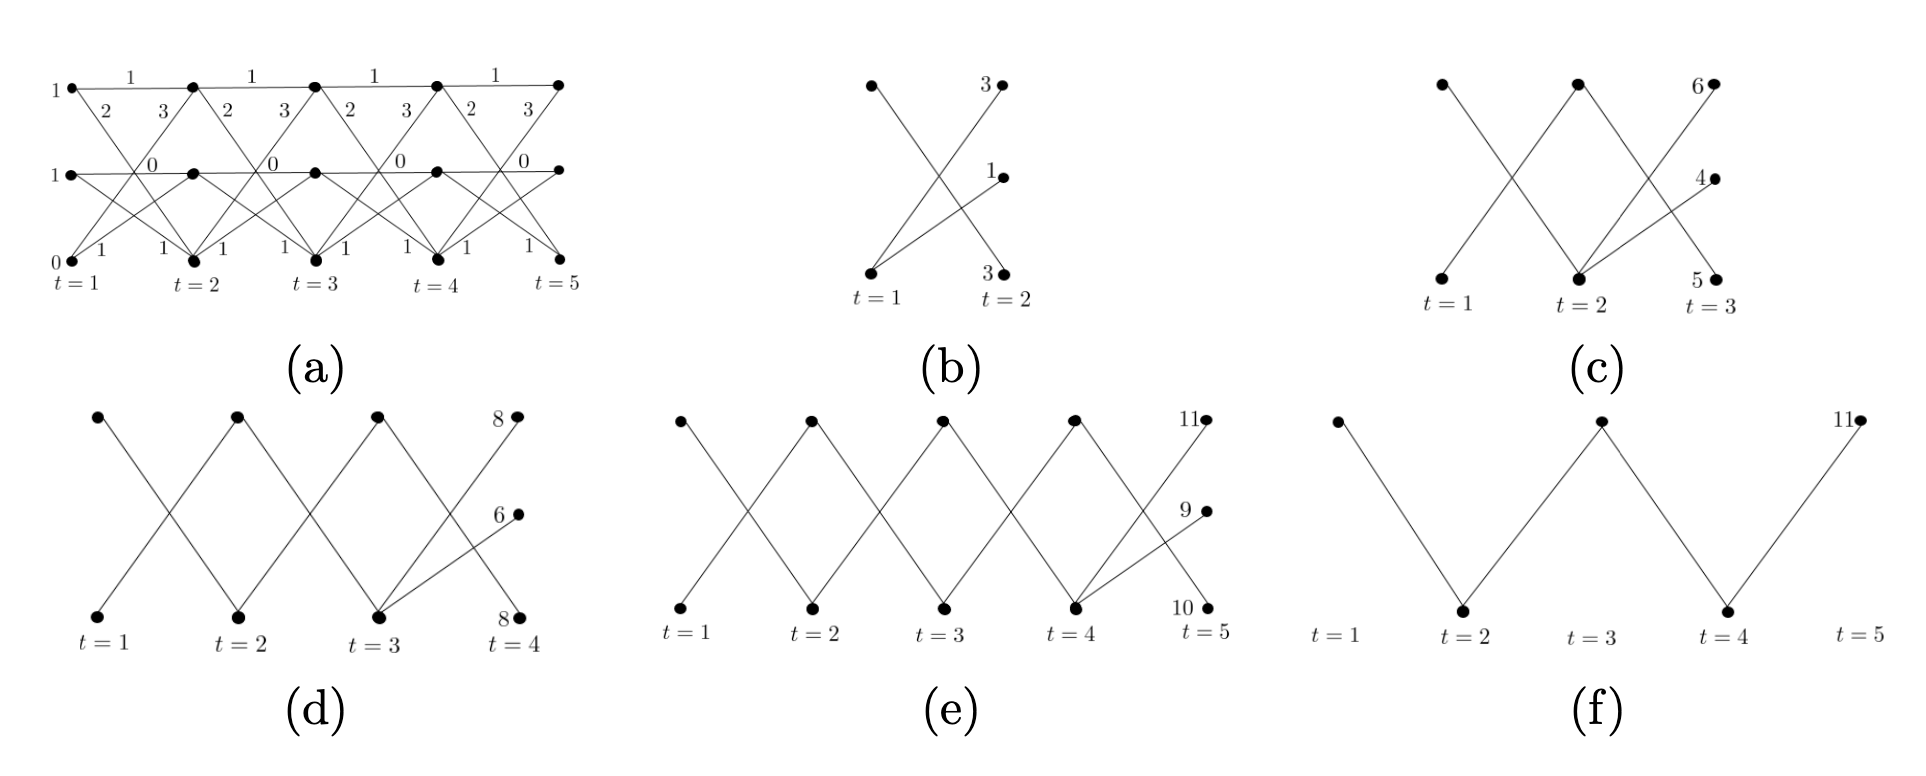
\includegraphics[scale=0.2]{dia.png}
    \caption{(a) Trellis diagram; (b)—(e) evolution of the Viterbi algorithm, showing surviving paths and values $V(t,x)$ at times $t = 2,3,4,5$; (f) optimal path $\vec{x}^* = (0,2,0,2,0)$ and its value $\varepsilon(\vec{x}^*) = 11$.}
    \label{}
\end{figure}\end{center}

\section{Bayesian Estimation of a Sequence: Need (MMSE) estimate $X_{1:t}$ given $Y_{1:t}$}
Consider Bayesian estimation under an additive squared-error loss function: $$L(\vec{x},\hat{\vec{x}})=\sum_{t=1}^nL(x_t,\hat{x}_t)=\sum_{t=1}^n\left(x_t-\hat{x}_t\right)^2$$
The Bayesian estimator $\hat{\vec{x}}$ achieves
\begin{equation}
    \begin{aligned}
        \min_{\hat{\vec{x}}}\sum_{\vec{x}\in X^n}L(\vec{x},\hat{\vec{x}})P(\vec{x}|\vec{y})=\sum_{t=1}^n\min_{\hat{\vec{x}}_t}\sum_{x_t\in X}L(x_t,\hat{x}_t)P(x_t|\vec{y})
    \end{aligned}
    \nonumber
\end{equation}
In particular, under squared-error loss, we obtain the conditional mean estimator
\begin{equation}
    \begin{aligned}
        \hat{\vec{x}}_t=\sum_{x_t\in X}x_t P\left(X_t=x|Y=\vec{y}\right),\quad 1\leq t\leq n
    \end{aligned}
    \nonumber
\end{equation}

\section{Forward-Backward Algorithm: (MMSE) estimate $X_{1:t+1}$ given $Y_{1:t}$}
\begin{enumerate}
    \item Evaluate $P\left(X_t=x|Y=\vec{y}\right)$ for $t=1,2,...,n$ and $x\in \mathcal{X}$. (Used to (MMSE) estimate $X_{1:t}$ given $Y_{1:t}$)
    \item Evaluate $P\left(X_t=x,X_{t+1}=x'|Y=\vec{y}\right)$ for $t=1,2,...,n$ and $x,x'\in \mathcal{X}$ (Used to learn parameters $\theta=(\pi,A,B)$)
\end{enumerate}
Define the shorthands
$$
\begin{aligned}
\gamma_t(x) & \triangleq \mathrm{P}\left\{X_t=x \mid \vec{Y}=\vec{y}\right\} \\
\xi_t\left(x, x^{\prime}\right) & \triangleq \mathrm{P}\left\{X_t=x, X_{t+1}=x^{\prime} \mid \vec{Y}=\vec{y}\right\}, \quad x, x^{\prime} \in \mathcal{X}
\end{aligned}
$$
Hence $\gamma_t$ is the first marginal of $\xi_t$. The forward-backward algorithm allows efficient computation of these probabilities.
\subsection{$\gamma_t(x) \triangleq \mathrm{P}\left\{X_t=x \mid \vec{Y}=\vec{y}\right\}$}
We begin with
$$
\gamma_t(x)=\mathrm{P}\left\{X_t=x \mid \vec{Y}=\vec{y}\right\}=\frac{\mathrm{P}\left\{X_t=x, \vec{Y}=\vec{y}\right\}}{\sum_{x \in \mathcal{X}} \mathrm{P}\left\{X_t=x, \vec{Y}=\vec{y}\right\}}, \quad 1 \leq t \leq n
$$
Write the numerator as a product of two conditional distributions,
$$
\begin{aligned}
\mathrm{P}\left\{\vec{Y}=\vec{y}, X_t=x\right\} & \stackrel{(a)}{=} \underbrace{\mathrm{P}\left\{Y_{1: t}=y_{1: t}, X_t=x\right\}}_{\mu_t(x)} \underbrace{\mathrm{P}\left\{Y_{t+1: n}=y_{t+1: n} \mid X_t=x\right\}}_{\nu_t(x)} \\
&=\mu_t(x) \nu_t(x), \quad 1 \leq t<n
\end{aligned}
$$
where (a) follows from the Markov chain $Y_{1: t} \rightarrow X_t \rightarrow Y_{t+1: n}$. For $t=n$, we let $\nu_n(x) \equiv 1$. Combining above two equations we have
$$
\gamma_t(x)=\frac{\mu_t(x) \nu_t(x)}{\sum_{x \in \mathcal{X}} \mu_t(x) \nu_t(x)} .
$$
\begin{enumerate}[(1)]
    \item The first factor in the product of $\mathrm{P}\left\{\vec{Y}=\vec{y}, X_t=x\right\}$ is
    $$
    \mu_t(x)=\mathrm{P}\left\{Y_{1: t}=y_{1: t}, X_t=x\right\}, \quad x \in \mathcal{X}, 1 \leq t \leq n,
    $$
    for which we derive a \textbf{forward recursion}. The recursion is initialized with
    $$
    \mu_1(x)=\mathrm{P}\left\{Y_1=y_1, X_1=x\right\}=\pi(x) B\left(x, y_1\right) .
    $$
    For $t \geq 1$ we express $\mu_{t+1}$ in terms of $\mu_t$ as follows:
    $$
    \begin{aligned}
    \mu_{t+1}(x) &=\mathrm{P}\left\{Y_{1: t+1}=y_{1: t+1}, X_{t+1}=x\right\} \\
    & \stackrel{(a)}{=} \mathrm{P}\left\{Y_{1: t}=y_{1: t}, X_{t+1}=x\right\} \mathrm{P}\left\{Y_{t+1}=y_{t+1} \mid X_{t+1}=x\right\} \\
    &=B\left(x, y_{t+1}\right) \sum_{x^{\prime} \in \mathcal{X}} \mathrm{P}\left\{Y_{1: t}=y_{1: t}, X_{t+1}=x, X_t=x^{\prime}\right\} \\
    & \stackrel{(b)}{=} B\left(x, y_{t+1}\right) \sum_{x^{\prime} \in \mathcal{X}} \mathrm{P}\left\{Y_{1: t}=y_{1: t}, X_t=x^{\prime}\right\} \mathrm{P}\left\{X_{t+1}=x \mid X_t=x^{\prime}\right\} \\
    &=B\left(x, y_{t+1}\right) \sum_{x^{\prime} \in \mathcal{X}} \mu_t\left(x^{\prime}\right) \mathrm{A}\left(x^{\prime}, x\right), \quad t=1,2, \cdots, n-1
    \end{aligned}
    $$
    where (a) holds because $Y_{1: t} \rightarrow X_{t+1} \rightarrow Y_{t+1}$ forms a Markov chain, and (b) because $Y_{1: t} \rightarrow X_t \rightarrow X_{t+1}$ forms a Markov chain.
    \item The second factor in the product of $\mathrm{P}\left\{\vec{Y}=\vec{y}, X_t=x\right\}$ is
    $$
    \nu_t(x)=\mathrm{P}\left\{Y_{t+1: n}=y_{t+1: n} \mid X_t=x\right\}, \quad x \in \mathcal{X}, 1 \leq t<n .
    $$
    Starting from $\nu_n(x) \equiv 1$, we have the following \textbf{backward recursion}, expressing $\nu_{t-1}$ in terms of $\nu_t$ for $2 \leq t \leq n$ :
    $$
    \begin{aligned}
    \nu_{t-1}(x) &=\mathrm{P}\left\{Y_{t: n}=y_{t: n} \mid X_{t-1}=x\right\} \\
    &=\sum_{x^{\prime} \in \mathcal{X}} \mathrm{P}\left\{Y_{t: n}=y_{t: n}, X_t=x^{\prime} \mid X_{t-1}=x\right\} \\
    & \stackrel{(a)}{=} \sum_{x^{\prime} \in \mathcal{X}} \mathrm{P}\left\{Y_{t: n}=y_{t: n} \mid X_t=x^{\prime}\right\} \mathrm{P}\left\{X_t=x^{\prime} \mid X_{t-1}=x\right\} \\
    & \stackrel{(b)}{=} \sum_{x^{\prime} \in \mathcal{X}} \mathrm{P}\left\{Y_{t+1: n}=y_{t+1: n} \mid X_t=x^{\prime}\right\} \mathrm{P}\left\{Y_t=y_t \mid X_t=x^{\prime}\right\} \mathrm{P}\left\{X_t=x^{\prime} \mid X_{t-1}=x\right\} \\
    &=\sum_{x^{\prime} \in \mathcal{X}} \nu_t\left(x^{\prime}\right) \mathrm{B}\left(x^{\prime}, y_t\right) \mathrm{A}\left(x, x^{\prime}\right), \quad t=n, n-1, \cdots, 2
    \end{aligned}
    $$
    where (a) holds because $X_{t-1} \rightarrow X_{t} \rightarrow Y_{t:n}$ forms a Markov chain, and (b) because $Y_{t+1: n} \rightarrow X_t \rightarrow Y_t$ forms a Markov chain.
\end{enumerate}

\subsection{$\xi_t\left(x, x^{\prime}\right) \triangleq \mathrm{P}\left\{X_t=x, X_{t+1}=x^{\prime} \mid \vec{Y}=\vec{y}\right\}$}
Next we derive an expression for
$$
\xi_t\left(x, x^{\prime}\right)=\mathrm{P}\left\{X_t=x, X_{t+1}=x^{\prime} \mid \vec{Y}=\vec{y}\right\}=\frac{\mathrm{P}\left\{\vec{Y}=\vec{y}, X_t=x, X_{t+1}=x^{\prime}\right\}}{\sum_{x, x^{\prime} \in \mathcal{X}} \mathrm{P}\left\{\vec{Y}=\vec{y}, X_t=x, X_{t+1}=x^{\prime}\right\}}
$$
We have
\begin{equation}
    \begin{aligned}
        \mathrm{P}&\left\{\vec{Y}=\vec{y}, X_t=x, X_{t+1}=x^{\prime}\right\}\\
        &\stackrel{(a)}{=} \mathrm{P}\left\{Y_{1: t+1}=y_{1: t+1}, X_t=x, X_{t+1}=x^{\prime}\right\} \mathrm{P}\left\{Y_{t+2: n}=y_{t+2: n} \mid X_{t+1}=x^{\prime}\right\}\\
        &\stackrel{(b)}{=} \mathrm{P}\left\{Y_{1: t}=y_{1: t}, X_t=x\right\} \mathrm{P}\left\{X_{t+1}=x^{\prime} \mid X_t=x\right\} \mathrm{P}\left\{Y_{t+1}=y_{t+1} \mid X_{t+1}=x^{\prime}\right\} \nu_{t+1}\left(x^{\prime}\right)\\
        &=\mu_t(x) \mathrm{A}\left(x, x^{\prime}\right) \mathrm{B}\left(x^{\prime}, y_{t+1}\right) \nu_{t+1}\left(x^{\prime}\right)
    \end{aligned}
    \nonumber
\end{equation}
where (a) holds because $\left(Y_{1: t+1}, X_t\right) \rightarrow X_{t+1} \rightarrow Y_{t+2: n}$ forms a Markov chain, and (b) because $Y_{1: t} \rightarrow X_t \rightarrow X_{t+1} \rightarrow Y_{t+1}$ forms a Markov chain. Hence
$$
\xi_t\left(x, x^{\prime}\right)=\frac{\mu_t(x) \mathrm{A}\left(x, x^{\prime}\right) \mathrm{B}\left(x^{\prime}, y_{t+1}\right) \nu_{t+1}\left(x^{\prime}\right)}{\sum_{x, x^{\prime} \in \mathcal{X}} \mu_t(x) \mathrm{A}\left(x, x^{\prime}\right) \mathrm{B}\left(x^{\prime}, y_{t+1}\right) \nu_{t+1}\left(x^{\prime}\right)}, \quad 1 \leq t \leq n, x, x^{\prime} \in \mathcal{X}
$$

\subsection{Scaling Factors}
Unfortunately the recursions above are numerically unstable for large $n$ because the probabilities $\mu_t(x)$ and $\nu_t(x)$ vanish exponentially with $n$ and are sums of many small terms of different sizes. The following approach is more stable. Define
$$
\begin{aligned}
\alpha_t(x) &=\mathrm{P}\left\{X_t=x \mid Y_{1: t}=y_{1: t}\right\}, \\
\beta_t(x) &=\frac{\mathrm{P}\left\{Y_{t+1: n}=y_{t+1: n} \mid X_t=x\right\}}{\mathrm{P}\left\{Y_{t+1: n}=y_{t+1: n} \mid Y_{1: t}=y_{1: t}\right\}}, \\
c_t &=\mathrm{P}\left\{Y_t=y_t \mid Y_{1: t-1}=y_{1: t-1}\right\}
\end{aligned}
$$
Then
$$
\begin{aligned}
\gamma_t(x) &=\alpha_t(x) \beta_t(x) \\
\xi_t\left(x, x^{\prime}\right) &=c_t \alpha_t(x) \mathrm{B}\left(x, y_t\right) \mathrm{A}\left(x, x^{\prime}\right) \beta_t\left(x^{\prime}\right)
\end{aligned}
$$
A forward recursion can be derived for $\alpha_t$ and $c_t$, and a backward recursion for $\beta_t$.

The time and storage complexity of the algorithm is $O\left(n|\mathcal{X}|^2\right)$.










\chapter{Graphic Models}
To compute $P(x_1,...,x_d)$, we can utilize the chain rule $P(x_1,...,x_d)=P(x_1)\prod_{i=2}^d P(x_i|x_{1:i-1})$. However, this approach becomes computationally expensive as the dimension $d$ increases.

Fortunately, when there are conditionally independent relationships between variables, such as $x_A \bot x_C | x_B$, we can reduce the computational cost.

In this section, we can employ graphical models to represent probabilistic relationships between variables, particularly when there are conditionally independent relationships present.
\section{Graph Theory}
\begin{enumerate}
    \item A graph $(V,E)$, $V$ is a set of \textit{vertices}, $E\subseteq V\times V$ is a set of ordered pairs of vertices, called \textit{edges}.
    
    An edge $(i,j)\in E$ is \textit{directed} if $(i,j)\notin E$; otherwise the edge is \textit{undirected}. We denote directed and undirected edges by the symbols $i \rightarrow j$ and $i\sim j$, respectively.
    \item \textbf{Directed and Undirected Graphs:} Graphs in which \textit{all} edges are directed (resp. undirected).
    \item \textbf{Subgraph:} a subgraph $(S,E_S)$ of $(V,E)$ is a subset $S\subset G$ with edges that have both endpoints in $S$.
    \item \textbf{Clique:} A set $C$ of vertices in an undirected graph is a \underline{clique} if either $C$ is a singleton, or \textbf{each pair of vertices in $C$ is linked by an edge}.\\
    That is, all vertices in $C$ are neighbors. The clique is \underline{maximal} if there is no larger clique that contains $C$.
    \item \textbf{Parent, Child:} Vertex $i$ is a \underline{parent} of vertex $j$ if $i \rightarrow j$, in which case $j$ is also called a \underline{child} of $i$. We denote by $\pi(j)$ the set of parents of $j$.
    \item \textbf{Path:} A \textit{path} of length $n$ from $i$ to $j$ is a sequence $i = k_0,k_1,...,k_n = j$ of distinct vertices such that ($k_{m-1},k_m) \in E$ for all $m = 1,... ,n$. We designate such a path by $i \rightarrow j$.
    \item \textbf{Connected Graph:} An undirected graph is \underline{connected} if there is a path between any pair of nodes. In general, the connected components of a graph are those subgraphs which are connected.
    \item \textbf{Cycle/Loop:} An $n-$cycle, or loop, is a path of length $n$ $i \rightarrow j$ with $i = j$.
    
    A directed graph without cycle is also called Directed Acyclic Graph (DAG)
    \item \textbf{Tree:} A tree is a connected, undirected graph without cycles; \textbf{it has a unique path between any two vertices}.
    \item \textbf{Rooted Tree:} A rooted tree is the directed acyclic graph obtained from a tree by choosing as vertex as root and directing all edges away from this root. Each vertex of a rooted tree has at most one parent.
    \item \textbf{Forest:} A forest is an undirected graph where all connected components are trees.
\end{enumerate}
\begin{center}\begin{figure}[htbp]
    \centering
    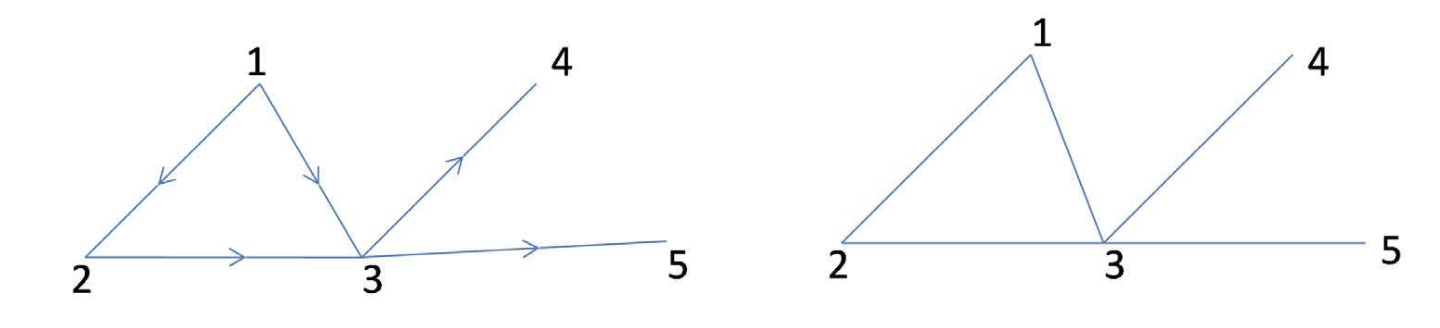
\includegraphics[scale=0.25]{graph.png}
    \caption{(a) Directed and (b) Undirected graph.}
    \label{}
\end{figure}\end{center}

\section{Bayesian Networks}
A Bayesian network (or belief network) is a joint probability distribution associated with a \textit{directed acyclic graph} $(V,E)$ whose nodes $X_v, v \in V$ are random variables. The joint distribution is of the form
\begin{equation}
    \begin{aligned}
        p(\vec{x})=\prod_{v\in V}p(x_v|\pi(x_v))
    \end{aligned}
    \nonumber
\end{equation}
$\pi(x_v)$ is the set of parents of vertices.

For instance a Markov chain is a chain-type directed acyclic graph where $V = \{1, 2,..., n\}$, and $\pi(v) = v - 1$ for $v \geq 2$. The pmf for the sequence $\vec{x}$ is obtained from the chain rule
\begin{equation}
    \begin{aligned}
        p(\vec{x})=p(x_1)p(x_2|x_1)\cdots p(x_n|x_{n-1})
    \end{aligned}
    \nonumber
\end{equation}

\section{Markov Networks}
\subsection{General Form}
We can use undirected graph to represent conditionally independent.
\begin{center}\begin{figure}[htbp]
    \centering
    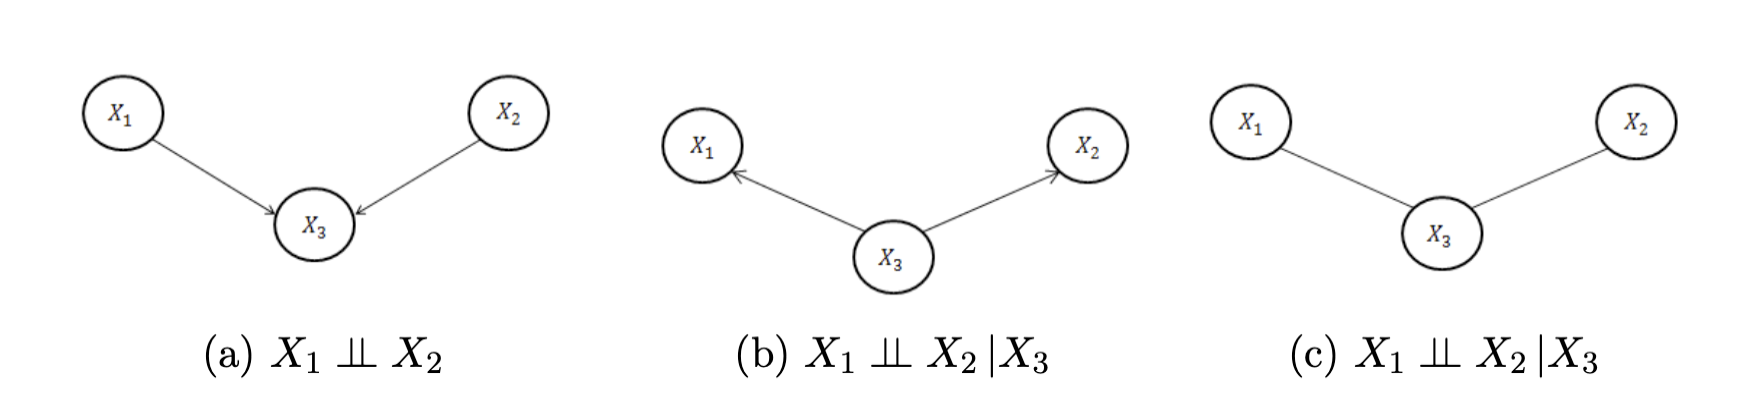
\includegraphics[scale=0.2]{BM.png}
    \caption{(a) (b) Two Bayesian networks and (c) a Markov network.}
    \label{}
\end{figure}\end{center}
More generally, if two nodes $X_u$ and $X_v$ in a Markov network are not connected by an edge, then the random variables $X_u$ and $X_v$ are conditionally independent given all the other random variables (denoted by $X_u \perp X_v \mid X_{\mathcal{V} \backslash\{u, v\}}$).

A Markov network is an undirected graph $G = (V,E)$ together with a collection $X = \{X_v, v \in V\}$ of random variables indexed by the nodes of $G$.

Since there is no direction, we use \textbf{clique} to help use represent probabilities. (\textit{Review: \underline{clique} is a set of vertices that each pair of vertices is linked})

We use $\Omega$ let be collection of cliques in the graph and the functions $\psi_C(\cdot)$ be the \textbf{\textit{clique potentials}, or \textit{compatibility functions}}.

The pmf of $X$ takes the form
\begin{equation}
    \begin{aligned}
        p(\vec{x})=\frac{\prod_{C\in \Omega}\psi_C(\vec{x}_C)}{\sum_{\vec{x}}\prod_{C}\psi_C(\vec{x}_C)}=\frac{1}{Z}\prod_{C\in \Omega}\psi_C(\vec{x}_C)
    \end{aligned}
    \nonumber
\end{equation}
where $Z=\sum_{\vec{x}}\prod_{C}\psi_C(\vec{x}_C)$ is a normalization constant.

\textbf{Note:} this is a form of factorization that can represent conditionally independent relationship among variables. $\psi_C(\cdot)$ are undefined functions.x

\subsection{Hammersley-Clifford theorem}
\begin{theorem}[Hammersley-Clifford theorem]
    Assume that $p\left(x_1, \ldots, x_n\right)>0$ (positivity condition). Then,
    $$
    p(\vec{x})=\frac{1}{Z} \prod_{\substack{C \in \Omega}} \phi_C\left(\vec{x}_C\right)
    $$
    Thus, the following are equivalent (given the positivity condition):
    \begin{enumerate}
        \item \textbf{Local Markov property:} $p\left(x_i \mid \vec{x} \backslash\left\{x_i\right\}\right)=p\left(x_i \mid \mathcal{N}\left(x_i\right)\right)$, where $\mathcal{N}\left(x_i\right)$ is the neighboring set of $x_i$.
        \item \textbf{Factorization property:} The probability factorizes according
        to the cliques of the graph.
        \item \textbf{Global Markov property:} $p\left(\vec{x}_A \mid \vec{x}_B, \vec{x}_S\right)=p\left(\vec{x}_A \mid \vec{x}_S\right)$
        whenever $\vec{x}_A$ and $\vec{x}_B$ are separated by $\vec{x}_S$ in $G$
    \end{enumerate}
\end{theorem}

\subsection{Form of Gibbs distribution (Boltzmann distribution)}
The factorization is not unique.
We let $\psi(\vec{x}_C)=e^{-V_C(\vec{x}_C)}$, where $V_C(\cdot)$ are the so-called potential energy functions. In a pairwise Markov network, $p(\vec{x})$ can be expressed as a product of clique potentials involving either one or two random variables.
\begin{equation}
    \begin{aligned}
        p(\vec{x})=\frac{1}{Z}e^{-\sum_CV_C(x_C)}
    \end{aligned}
    \nonumber
\end{equation}
This probability follows \textbf{Gibbs distribution (Boltzmann distribution)}. This distribution follows exponential families.

\section{Conversion of directed graph to undirected graph}
We can use a step known as \textit{moralization}.
Moralization of graph: connect two unmarried parents.

This is the process of “marrying” the parents of each node, i.e., adding an edge connecting any pair of parents if one did not exist. The figure illustrates this process for a node with three parents. In this case the undirected graph consists of a clique of size 4.
\begin{center}\begin{figure}[htbp]
    \centering
    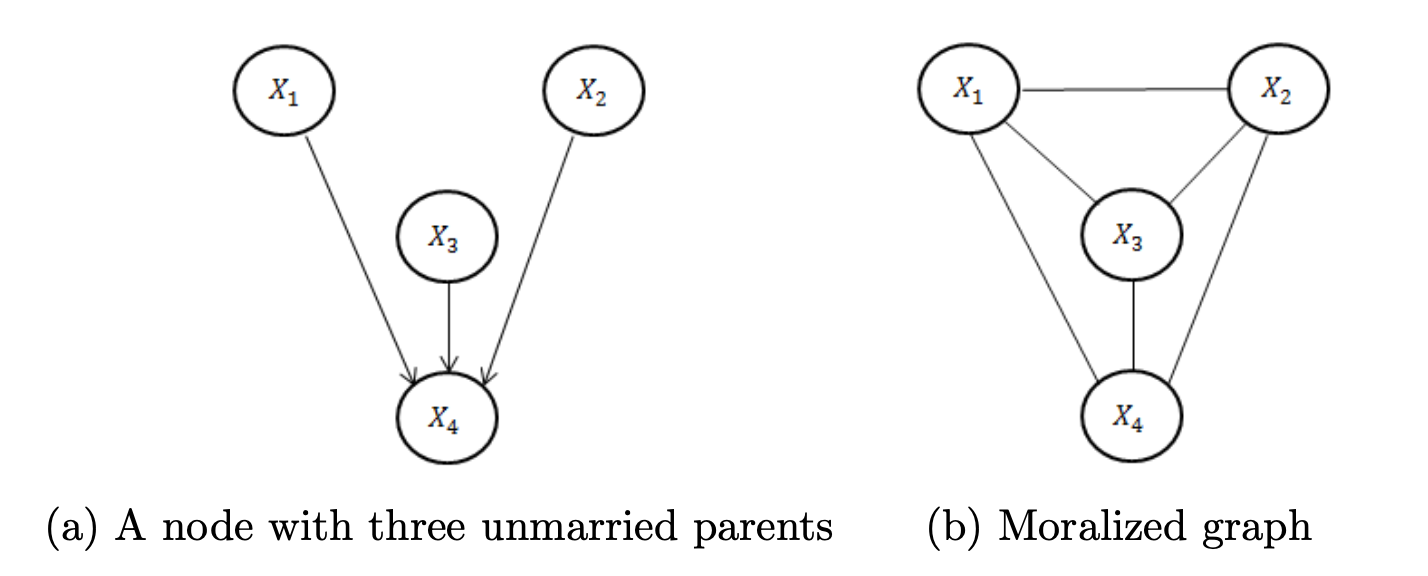
\includegraphics[scale=0.25]{moralization.png}
    \caption{Graph moralization}
    \label{}
\end{figure}\end{center}

\section{ Inference and Learning}
\subsection{Inference on Trees}
Consider the tree of the figure, which has 5 nodes and edges $1\sim 2\sim 3$ and $4\sim 3\sim 5$. We have
\begin{equation}
    \begin{aligned}
        p(\vec{x})=\frac{1}{Z}\psi_{12}(x_1,x_2)\psi_{23}(x_2,x_3)\psi_{34}(x_3,x_4)\psi_{35}(x_3,x_5)
    \end{aligned}
    \nonumber
\end{equation}
\begin{center}\begin{figure}[htbp]
    \centering
    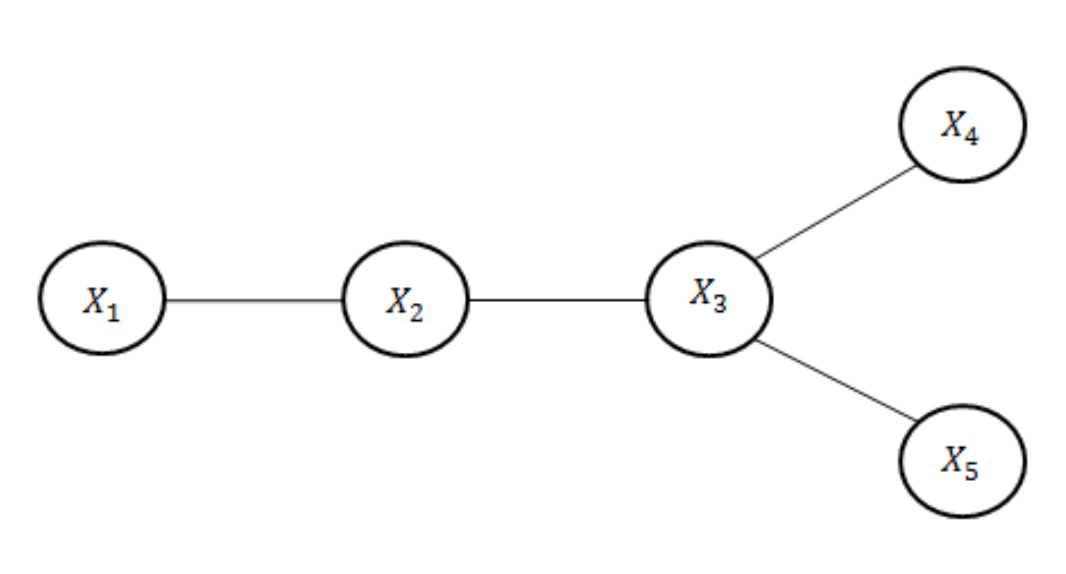
\includegraphics[scale=0.2]{inftree.png}
    \caption{Example 1}
    \label{}
\end{figure}\end{center}
\begin{enumerate}
    \item \textbf{Marginal Inference:} As a first example of inference on trees, consider the problem of evaluating the marginal pmf $p(x_5)$. We explore two approaches: the \textbf{direct approach}, which is computationally infeasible for large graphs (the number of items in the sum is $|\mathcal{X}|^4$);
    $$p(x_5)=\sum_{x_1,...,x_4}\frac{1}{Z}\psi_{12}(x_1,x_2)\psi_{23}(x_2,x_3)\psi_{34}(x_3,x_4)\psi_{35}(x_3,x_5)$$
    and the \textbf{sum-product algorithm}, which exploits the graph structure.
    $$
    \begin{aligned}
    p\left(x_5\right) &=\frac{1}{Z} \sum_{x_3} \psi_{35}\left(x_3, x_5\right) \sum_{x_4} \psi_{34}\left(x_3, x_4\right) \sum_{x_2} \psi_{23}\left(x_2, x_3\right) \underbrace{\sum_{x_1} \psi_{12}\left(x_1, x_2\right)}_{m_{1 \rightarrow 2}\left(x_2\right)} \\
    &=\frac{1}{Z} \sum_{x_3} \psi_{35}\left(x_3, x_5\right) \sum_{x_4} \psi_{34}\left(x_3, x_4\right) \underbrace{\sum_{x_2} \psi_{23}\left(x_2, x_3\right) m_{1 \rightarrow 2}\left(x_2\right)}_{m_{2 \rightarrow 3}\left(x_3\right)} \\
    &=\frac{1}{Z} \sum_{x_3} \psi_{35}\left(x_3, x_5\right) m_{2 \rightarrow 3}\left(x_3\right) \underbrace{\sum_{x_4} \psi_{34}\left(x_3, x_4\right)}_{m_{4 \rightarrow 3}\left(x_3\right)} \\
    &=\frac{1}{Z} \underbrace{\sum_{x_3} \psi_{35}\left(x_3, x_5\right) m_{2 \rightarrow 3}\left(x_3\right) m_{4 \rightarrow 3}\left(x_3\right)}_{m_{3 \rightarrow 5}\left(x_5\right)} .
    \end{aligned}
    $$
    In this derivation, nodes $1,2,4,3$ are eliminated in that order. We think of each term $m_{i \rightarrow j}\left(x_j\right)$ as a message conveyed from node $i$ to node $j$, just before elimination of $j$. Computing $m_{i \rightarrow j}\left(x_j\right)$ involves a summation over all possible values of $x_i$. This interpretation will be helpful in more complex problems.
    \begin{center}\begin{figure}[htbp]
        \centering
        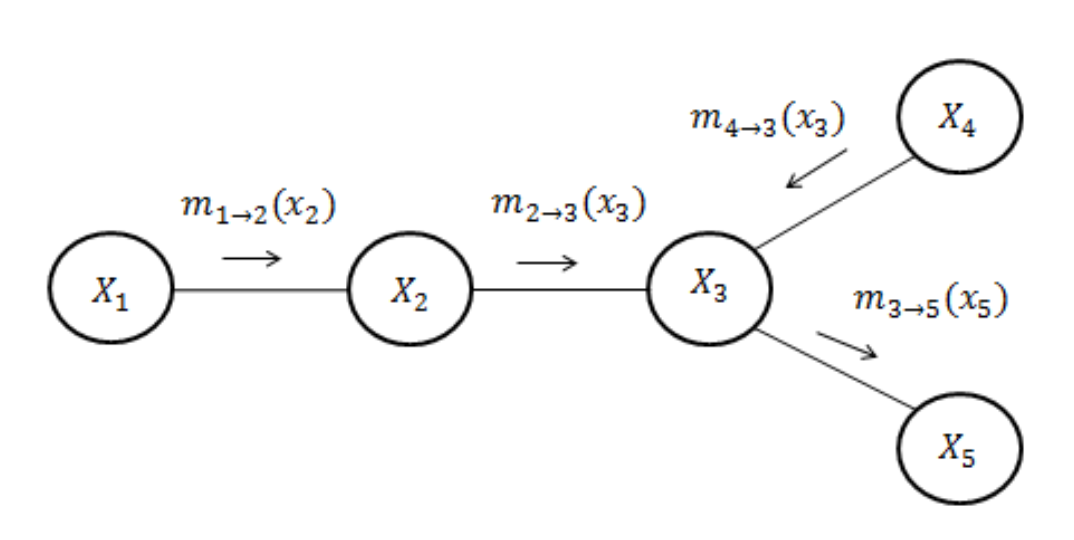
\includegraphics[scale=0.2]{belief.png}
        \caption{Belief propagation in a tree}
        \label{}
    \end{figure}\end{center}
    As illustrated in the Figure, a node can send a message to a neighbor once it has received messages from all of its other neighbors. For a general tree, upon choosing an elimination order, we evaluate the following messages in the corresponding order:
    $$
    m_{i \rightarrow j}\left(x_j\right)=\sum_{x_i} \psi_{i j}\left(x_i, x_j\right) \prod_{k \in \mathcal{N}(i) \backslash\{j\}} m_{k \rightarrow i}\left(x_i\right)
    $$
    The marginal probability at any node $i$ is the product of all incoming messages:
    $$
    p\left(x_i\right)=\frac{1}{Z} \prod_{k \in \mathcal{N}(i)} m_{k \rightarrow i}\left(x_i\right) .
    $$
    We can also evaluate the 2D marginal $p(x_2,x_5)$
    $$
    p\left(x_2, x_5\right)=\frac{1}{Z} \sum_{x_3} \psi_{23}\left(x_2, x_3\right) \psi_{35}\left(x_3, x_5\right) \underbrace{\sum_{x_4} \psi_{34}\left(x_3, x_4\right)}_{m_{4 \rightarrow 3}\left(x_3\right)} \underbrace{\sum_{x_1} \psi_{12}\left(x_1, x_2\right)}_{m_{1 \rightarrow 2}\left(x_2\right)} .
    $$
    Finally, a conditional marginal such as $p\left(x_1 \mid x_5\right)$ is obtained as $p\left(x_1, x_5\right) / p\left(x_5\right)$, hence the problem is reduced to evaluating unconditional marginals.

    The computational cost of the algorithm is $O\left(n|\mathcal{X}|^2\right)$ when the $n$ random variables are defined over the same alphabet $\mathcal{X}$.

    \item \textbf{Maximization:} A closely related problem is to find the most likely configuration, possibly by fixing some coordinates. For instance, evaluate
    $$
    M\left(x_5\right)=\max _{x_1, x_2, x_3, x_4} p\left(x_1, x_2, x_3, x_4, x_5\right)
    $$
    for the above Markov network. Direct calculation has exponential complexity. However, the more efficient max-product algorithm has the same structure as the sum-product algorithm:
    \begin{equation}
        \begin{aligned}
            M\left(x_5\right)&=\max _{x_1, x_2, x_3, x_4} \frac{1}{Z} \psi_{12}\left(x_1, x_2\right) \psi_{23}\left(x_2, x_3\right) \psi_{34}\left(x_3, x_4\right) \psi_{35}\left(x_3, x_5\right)\\
            &=\frac{1}{Z} \max _{x_3} \psi_{35}\left(x_3, x_5\right) \max _{x_4} \psi_{34}\left(x_3, x_4\right) \max _{x_2} \psi_{23}\left(x_2, x_3\right) \underbrace{\max _{x_1} \psi_{12}\left(x_1, x_2\right)}_{m_{1 \rightarrow 2}\left(x_2\right)}\\
            &=\frac{1}{Z} \max _{x_3} \psi_{35}\left(x_3, x_5\right) \underbrace{\max _{x_4} \psi_{34}\left(x_3, x_4\right)}_{m_{4 \rightarrow 3}\left(x_3\right)} \underbrace{m_{x_2} \psi_{23}\left(x_2, x_3\right) m_{1 \rightarrow 2}\left(x_2\right)}_{m_{2 \rightarrow 3}\left(x_3\right)}\\
            &=\frac{1}{Z} \underbrace{\max _{x_3} \psi_{35}\left(x_3, x_5\right) m_{4 \rightarrow 3}\left(x_3\right) m_{2 \rightarrow 3}\left(x_3\right)}_{m_{3 \rightarrow 5}\left(x_5\right)}
        \end{aligned}
        \nonumber
    \end{equation}
\end{enumerate}





















\chapter{Variational Inference, Mean-Field Techniques}
Approximate complicated p.d.f. $p(\vec{x})$ with tractable $q(\vec{x})$, where $q\in Q=$ tractable set of distributions.

Use divergence to measure:
\begin{equation}
    \begin{aligned}
        \min_{q\in Q}\quad D(q\| p)
    \end{aligned}
    \nonumber
\end{equation}
note that $D$ is convex in $q$.

\section{Naive Mean-Field Methods}
The \textit{naive mean field method} approximates a distribution by a product distribution.

Assume the $q$ has the form $q(\vec{x})=\prod_{i=1}^nq_i (x_i)$. Assume $x_i\in X=$ finite set.
\begin{equation}
    \begin{aligned}
        D(q\| p)&=\mathbb{E}_q\left[\ln\frac{q(\vec{X})}{p(\vec{X})}\right]\\
        &=\sum_{i=1}^n \mathbb{E}_{q}\left[\ln q_i(X_i)\right]- \mathbb{E}_q\left[\ln p(\vec{X})\right]\\
        &=\sum_{i=1}^n\sum_{x_i\in X}q_i(x_i)\ln q_i(x_i)-\sum_{\vec{x}\in X^n}\left(\prod_{i=1}^nq_i (x_i)\right)\ln p(\vec{x})
    \end{aligned}
    \nonumber
\end{equation}

Solve 
\begin{equation}
    \begin{aligned}
        \min_{\{q_i\}}&\quad D(\prod_{i=1}^nq_i\| p)\\
        s.t.&\sum_{x_i\in X}q_i(x_i)=1,i=1,...,n
    \end{aligned}
    \nonumber
\end{equation}
Using Lagrangian method:
\begin{equation}
    \begin{aligned}
        L(q,\vec{\lambda})&=D(q\| p)+\sum_{i=1}^n\lambda_i\left(\sum_{x\in X}q_i(x_i)-1\right)\\
        0=\frac{\partial L(q,\vec{\lambda})}{\partial q_i(x_i)}&=1+\ln q_i(x_i)-\sum_{\vec{x}':x'_i=x_i}\left(\prod_{j\neq i}^nq_j (x'_j)\right)\ln p(\vec{x}')+\lambda_i
    \end{aligned}
    \nonumber
\end{equation}
Hence, $q_i(x_i)$ should in the form:
\begin{equation}
    \begin{aligned}
        q_i(x_i)&=\frac{1}{e^{1+\lambda_i}}e^{\sum_{\vec{x}':x'_i=x_i}\left(\prod_{j\neq i}^nq_j (x'_j)\right)\ln p(\vec{x}')}\\
        &=\frac{1}{Z_i}exp\left({\mathbb{E}_{\prod_{j\neq i}^nq_j}[\ln p(X_{1:i-1},x_i,X_{i+1:n})]}\right)
    \end{aligned}
    \nonumber
\end{equation}
Iteration Algorithm:
\begin{equation}
    \begin{aligned}
        q_i^{(k+1)}(x_i)=\frac{1}{Z_i}exp\left({\mathbb{E}_{\prod_{j\neq i}^nq_j^{(k)}}[\ln p(X_{1:i-1},x_i,X_{i+1:n})]}\right)
    \end{aligned}
    \nonumber
\end{equation}

\subsection{Graphical Models}
Consider $P=$ pairwise Markov model
\begin{equation}
    \begin{aligned}
        p(\vec{x})&=\frac{1}{Z}\prod_{(i,j)\in E}\psi_{ij}(x_i,x_j)\\
        \ln p(\vec{x})&=-\ln{Z}+\sum_{(i,j)\in E}\ln\psi_{ij}(x_i,x_j)\\
    \end{aligned}
    \nonumber
\end{equation}
The expectation can be written as
\begin{equation}
    \begin{aligned}
        {\mathbb{E}_{\prod_{j\neq i}^nq_j}[\ln p(X_{1:i-1},x_i,X_{i+1:n})]}&=\mathbb{E}_{\prod_{j\neq i}^nq_j}[\sum_{(i,j)\in E}\ln\psi_{ij}(x_i,x_j)]+cst\\
        &=\sum_{j\in N(i)}\mathbb{E}_{q_j}[\ln\psi_{ij}(x_i,x_j)]+cst\\
        &=\sum_{j\in N(i)}\sum_{x_j\in X}q_j(x_j)\ln\psi_{ij}(x_i,x_j)+cst
    \end{aligned}
    \nonumber
\end{equation}
and thus,
\begin{equation}
    \begin{aligned}
        q_i(x_i)
        &=\frac{1}{Z_i}exp\left(\sum_{j\in N(i)}\sum_{x_j\in X}q_j(x_j)\ln\psi_{ij}(x_i,x_j)\right)
    \end{aligned}
    \nonumber
\end{equation}

\subsection{Ising Model}
Consider a 2-D torus $V$ with $|V| = n$ nodes, and $X = \{\pm 1\}$. Each node is connected to its upper, lower, right, and left neighbors. The distribution is of the form
\begin{equation}
    \begin{aligned}
        p(\vec{x})=\frac{1}{Z}exp\left(\beta\sum_{(i,j)\in E}x_ix_j\right),\quad \vec{x}\in \{\pm 1\}^n
    \end{aligned}
    \nonumber
\end{equation}
with $\beta \geq 0$. The parameter $\beta$ represents the inverse of a temperature. For $\beta = 0$ the distribution is uniform, hence fully factorized. For large positive values of $\beta$, configurations $\vec{x}$ with strong correlations are favored.

\textbf{2-D Ising Model}
$$\psi_{ij}(x_i,x_j)=e^{\beta x_ix_j}$$
\begin{equation}
    \begin{aligned}
        \Rightarrow q_i(x_i)=\frac{1}{Z_i}\prod_{j\in N(i)}exp\left(-\sum_{x_j=\pm 1}q_j(x_j)\beta x_i x_j\right)
    \end{aligned}
    \nonumber
\end{equation}

Since each $X_i$ is a Bernoulli random variable, the decision varibale $q_i$ can be represented by a single parameter which we choose to be the mean $m_i = q_i(1) - q_i(-1) \in [-1, 1]$. Equivalently,
\begin{equation}
    \begin{aligned}
        m_i = q_i(1) - q_i(-1)&\Leftrightarrow q_i(1)=\frac{1+m_i}{2},\ q_i(-1)=\frac{1-m_i}{2}\\
        &\Rightarrow q_i(x_i)=\frac{1}{Z_i}\prod_{j\in N(i)}exp\left(-\beta x_i m_j\right)
    \end{aligned}
    \nonumber
\end{equation}
Then, our problem is finding the optimal $\{m_i\}$.

\begin{equation}
    \begin{aligned}
        q_i(1)=\frac{1}{Z_i}exp\left(-\beta\sum_{j\in N(i)} m_j\right);\ q_i(-1)=\frac{1}{Z_i}exp\left(\beta\sum_{j\in N(i)} m_j\right)
    \end{aligned}
    \nonumber
\end{equation}
The normalization constant is given by
\begin{equation}
    \begin{aligned}
        Z_i=exp\left(\beta\sum_{j\in N(i)} m_j\right)+exp\left(-\beta\sum_{j\in N(i)} m_j\right)=2{cosh}\left(\beta\sum_{j\in N(i)}m_j\right)
    \end{aligned}
    \nonumber
\end{equation}
Hence, $$m_i=q_i(1)-q_i(-1)={tanh}\left(\beta\sum_{j\in N(i)}m_j\right)$$
\textbf{Convergence}. We show that the algorithm always converges if a uniform initialization is used, i.e., $m_i^{(0)} = m^{(0)}$ for all $i \in V$. Then the (simultaneous) update equation for the means is
\begin{equation}
    \begin{aligned}
        m^{(k+1)}={tanh}\left(4\beta m^{(k)}\right)
    \end{aligned}
    \nonumber
\end{equation}
where the factor of $4$ arises because each vertex has $4$ neighbors. Analysis of convergence depends on the value of $\beta$, and we need consider two cases.
\begin{enumerate}[(1)]
    \item \textbf{Case I: $\beta < \frac{1}{4}$:} The mapping is a contraction mapping for $\beta<\frac{1}{4}$, and so the fixed point of this mapping is $\lim_{k \rightarrow \infty} m^{(k)} = 0$, for any initialization $m^{(0)}$. Hence, the variational approximation is uniform: $q(\vec{x}) = 2^{-n}$ for all $x \in \{\pm 1\}^V$.
    \item \textbf{Case II: $\beta > \frac{1}{4}$:} In this case, the equation $m=\tanh (4 \beta m)$ has three possible solutions 0 and $\pm m^*$ where $m^*>0$. If the algorithm is initialized with $m^{(0)}=0$, then subsequent iterations do not change this value. If the algorithm is initialized with $m^{(0)}>0$, it converges to $m^*$. Finally, if the algorithm is initialized with $m^{(0)}<0$, it converges to $-m^*$. In the latter two cases (convergence to either $m^*$ or $-m^*$), the variational approximations $q_i$ are nonuniform.
    \item \textbf{Case III: $\beta = \frac{1}{4}$:} phase transition
\end{enumerate}
The case $\beta>\frac{1}{4}$ is related to percolation theory in statistical physics. It may be shown that the distribution $p$ favors configurations featuring large homogeneous regions. The correlation between any two nodes is significant, even for large graphs. This behavior is completely different from the case $\beta<\frac{1}{4}$, where the correlation between distant nodes dies out with distance (similarly to a homogeneous, irreducible Markov chain). The case $\beta=\frac{1}{4}$ is known as a phase transition.

\section{Exponential Families of Probability Distributions}
\begin{definition}[$d-$dimensional exponential families]
    In canonical form: $d-$dimensional exponential families
    $$p_\theta(y)=\frac{h(y)}{Z(\theta)} e^{\sum_{k=1}^d\theta_k T_k(y)}$$
    $T_k (\cdot)$ are called sufficient statistics. \textbf{Partition function} $Z(\theta)$ is the normalization constant ensuring that the density $p_\theta$ integrates to $1$.\\
    It can also be written
    $$p_\theta(y)=e^{\theta^T T(y)-A(\theta)}$$
    The \textbf{log partition function} (aka cumulant function) $A(\theta) = ln Z(\theta)$
\end{definition}

\textbf{Example 1:} $P_\theta=N(\theta,1)$, $$p_\theta(y)=\frac{1}{\sqrt{2\pi}}e^{-\frac{(y-\theta)^2}{2}}=\frac{e^{\frac{y^2}{2}}}{\sqrt{2\pi}e^{-\frac{\theta^2}{2}}}e^{-\theta y}$$

\textbf{Example 2:} $P_\theta=N(0,\theta^{-1})$, $\theta$ is the inverse covariance matrix. $$p_\theta(y)=\frac{|\theta|^{\frac{1}{2}}}{\sqrt{2\pi}}e^{-\frac{1}{2}y^T\theta y}$$

\textbf{Example 3:} 2D-Ising Model $$p_\theta(y)=\frac{1}{Z(\theta)}e^{\theta y_iy_j},\theta>0$$
Generalized 2D-Ising Model $$p_\theta(y)=\frac{1}{Z(\theta)}e^{\sum_{i\in V}\theta_i y_i +\sum _{i\sim j}\theta_{ij} y_iy_j}$$

The natural parameter set:
$$\Theta=\{\theta:\int_X e^{\theta^T T(y)}dy<\infty\}$$

The divergence in exponential form
\begin{equation}
    \begin{aligned}
        D(P_\theta\| P_{\theta'})&=\mathbb{E}_\theta \left[\ln \frac{P_\theta (Y)}{P_{\theta'} (Y)}\right]\\
        &=\mathbb{E}_\theta[\theta^T T(Y)-A(\theta)-(\theta')^T T(Y)+A(\theta')]\\
        &=-[A(\theta)-A(\theta')]+(\theta-\theta')^T \mathbb{E}_\theta [T(Y)]
    \end{aligned}
    \nonumber
\end{equation}

\textbf{Cumulant-generating function} (cgf)
\begin{equation}
    \begin{aligned}
        \kappa(u)=\ln \mathbb{E}(e^{u^TT(Y)})=\ln \int e^{u^TT(y)}(e^{\theta^T T(y)-A(\theta)}) dy
    \end{aligned}
    \nonumber
\end{equation}
\begin{equation}
    \begin{aligned}
    \nabla \kappa(0)&=\mathbb{E}_\theta[T(Y)] \\
    \nabla^2 \kappa(0)&=\operatorname{Cov}_\theta[T(Y)]
    \end{aligned}
    \nonumber
\end{equation}

We can compute
\begin{equation}
    \begin{aligned}
        \int e^{\theta^T T(y)-A(\theta)} dy&=1\\
        \int [T(y)-\nabla A(\theta)] e^{\theta^T T(y)-A(\theta)} dy&=0\\
        \int[T(y)-\nabla A(\theta)]p_\theta(y) dy&=0\\
        \mathbb{E}_\theta [T(Y)]&=\nabla A(\theta)
    \end{aligned}
    \nonumber
\end{equation}
Hence,
\begin{equation}
    \begin{aligned}
    \nabla A(\theta) &=\nabla \kappa(0)=\mathbb{E}_\theta[T(X)] \\
    \nabla^2 A(\theta) &=\nabla^2 \kappa(0)=\operatorname{Cov}_\theta[T(X)]
    \end{aligned}
    \nonumber
\end{equation}

Definition. The set of realizable mean parameters $\mathcal{M}$ is the set of $\mu$ that are the expected value of $T(X)$ under some distribution $p$ (not necessarily in the exponential family). Thus
$$
\mathcal{M} \triangleq\left\{\mu \in \mathbb{R}^d: \exists p: \mathbb{E}_p[T(X)]=\mu\right\}
$$
which is a convex set.\\

\textbf{Example 6.} Consider Generalized 2D-Ising Model $$p_\theta(y)=\frac{1}{Z(\theta)}e^{\sum_{i\in V}\theta_i y_i +\sum _{i\sim j}\theta_{ij} y_iy_j}$$
For $y\in\{0,1\}$
\begin{equation}
    \begin{aligned}
        \mu_i&=\mathbb{E}_\theta \left[T_i(Y)\right]=P_\theta (Y_i=1)\\
        \mu_{ij}&=\mathbb{E}_\theta \left[T_i(Y)T_j(Y)\right]=P_\theta (Y_i=Y_j=1)\\
    \end{aligned}
    \nonumber
\end{equation}
\textbf{Example 7.} If $T(x)=x x^{\top} \in \mathbb{R}^{n \times n}$ then $\mu$ is a correlation matrix, and so $\mathcal{M}$ is the set of all $n \times n$ symmetric nonnegative definite matrices.

\section{ML Estimation}
Consider $n$ iid samples $X^{(i)}, 1 \leq i \leq n$ drawn from the exponential distribution $p_\theta$. The ML estimator of $\theta$ given these $n$ samples is obtained by solving
$$
\begin{aligned}
\hat{\theta}_{ML}&=\max _\theta \frac{1}{n} \sum_{i=1}^n \ln p_\theta\left(X^{(i)}\right)\\
&=\max _\theta \frac{1}{n} \sum_{i=1}^n\left[\theta^{\top} T\left(X^{(i)}\right)-A(\theta)\right] \\
&=\max _\theta\left[\theta^{\top} \hat{\mu}-A(\theta)\right]
\end{aligned}
$$
where $\hat{\mu}$ is the mean parameter
$$
\hat{\mu} \triangleq \frac{1}{n} \sum_{i=1}^n T\left(X^{(i)}\right)
$$
$A(\theta)$ is a convex function, we can solve optimal solution by solving critical point.
\begin{equation}
    \begin{aligned}
        \nabla A(\hat{\theta}_{ML})=\hat{\mu}
    \end{aligned}
    \nonumber
\end{equation}
The gradient mapping could be hard to invert, however. For instance, for the Ising model example we easily obtain
$$
\hat{\mu}=\frac{1}{n} \sum_{i=1}^n \sum_{j \sim k} X_j^{(i)} X_k^{(i)}
$$
but inverting the gradient mapping is a hard problem. Such is generally the case if $p$ is a distribution over a Markov network with cycles.

\section{Maximum Entropy}
Consider a random variable $X$ over a finite set $\mathcal{X}$. Its probability distribution $p$ is unknown, however we are given the expected value $\mu_k=\mathbb{E}_p\left[T_k(X)\right]$ of $d$ statistics $T_k(X), 1 \leq k \leq d$. A classical problem, which originates from statistical physics, is to find $p$ that maximizes the entropy $H(p)=-\sum_x p(x) \ln p(x)$ subject to the $d$ constraints above. Assuming the feasible set is nonvoid, the resulting distribution is called the maximum-entropy (or maxent()) distribution.

Since $H(p)$ is concave, the constraints are linear in $p$, and the probability simplex is a convex set, the maxent problem is concave. Its solution is obtained by introducing $d$ Lagrange multipliers $\lambda_k, 1 \leq k \leq d$ associated with the mean constraints, and a Lagrange multiplier $\lambda_{d+1}$ associated with the constraint $\sum_x p(x)=1$. Ignoring momentarily the nonnegativity constraints, we maximize the Lagrangian
$$
\mathcal{L}(p, \lambda) \triangleq-\sum_{x \in \mathcal{X}} p(x) \ln p(x)+\sum_{k=1}^d \lambda_k\left(\sum_{x \in \mathcal{X}} p(x) T_k(x)-\mu_k\right)+\lambda_{d+1}\left(\sum_{x \in \mathcal{X}} p(x)-1\right)
$$
over $p$, subject to the $d+1$ equality constraints

The first-order optimality conditions are given by
\begin{equation}
    \begin{aligned}
        0=\frac{\partial \mathcal{L}(p, \lambda)}{\partial p(x)}=-\ln p(x)-1+\sum_{k=1}^d\lambda_kT_k(x)+\lambda_{d+1}
    \end{aligned}
    \nonumber
\end{equation}
Hence, $$p(x)=\frac{1}{Z}e^{\sum_{k=1}^d\lambda_kT_k(x)}$$
where $Z=e^{1-\lambda_{d+1}}$

\begin{equation}
    \begin{aligned}
        H(p)=\mathbb{E}_p[\ln p(X)]=-\theta^T \mathbb{E}_p[T(X)]+A(\theta)=-\max_\theta(\theta^T \mu-A(\theta))
    \end{aligned}
    \nonumber
\end{equation}

\textbf{Example.} Let $X=\left(X_1, X_2\right) \in\{0,1\}^2$ and consider maximizing entropy subject to the constraint $\mathbb{E}\left[X_1 X_2\right]=\mu$ where $\mu \in(0,1)$. We obtain $p(x)=\frac{1}{Z} \exp \left\{\lambda x_1 x_2\right\}$. Since $\sum_x p(x)=1$, the normalization constant is obtained as $Z=e^\lambda+3$. We obtain $\lambda$ from the constraint
$$
\mu=\mathbb{E}_P\left[X_1 X_2\right]=\frac{e^\lambda}{e^\lambda+3} \quad \Rightarrow \quad \lambda=\ln \frac{3 \mu}{1-\mu}
$$
The maxent solution takes the form
$$
p(x)=\left\{\begin{matrix}
    \mu &\left(x_1, x_2\right)=(1,1) \\ \frac{1-\mu}{3} & \text { else }
\end{matrix}\right.
$$
and has entropy is $H(p)=-\mu \ln \mu-(1-\mu) \ln \frac{1-\mu}{3}$.\\
A similar version of the maxent problem exists for continuous random variables. The entropy function is replaced with the differential entropy functional $h(p) \triangleq-\int p \ln p$, and the maxent solution again takes an exponential form.


\section{}
\begin{equation}
    \begin{aligned}
        \min_{q\in Q}\ D(q\| p)&=\min_q \mathbb{E}_q\left[\ln\frac{q(x)}{p_\theta(x)}\right]\\
        &=\min_q \left[A(\theta)-\theta^T \mathbb{E}_q[T(x)]-H(q)\right]\\
        &=A(\theta)-\max_\mu \max_{q: \mathbb{E}_q[T(x)]=\mu}\left[\theta^T \mathbb{E}_q [T(x)]+H(q)\right]\\
        &=A(\theta)-\max_{\mu\in M}\left[\theta^T \mu +\max_{q: \mathbb{E}_q[T(x)]=\mu}H(q)\right]
    \end{aligned}
    \nonumber
\end{equation}
Since $\max_{q: \mathbb{E}_q[T(x)]=\mu}H(q)$ is exactly an entropy maximum problem, we let $A^*(\mu)=\max_{q: \mathbb{E}_q[T(x)]=\mu}H(q)$.

As we showed: (1). $A^*(\mu)=\max_\theta [\theta^T\mu- A(\theta)]$, $A(\theta)=\max_\mu [\theta^T\mu-A^*(\mu)]$
\begin{equation}
    \begin{aligned}
        \min_{q\in Q}\ D(q\| p)&=A(\theta)-\max_{\mu\in M}\left[\theta^T \mu +A^*(\mu)\right]
    \end{aligned}
    \nonumber
\end{equation}


\section{Connection between Exponential Families and Graphic Models}

Pairwise Markov network over $G(V,E)$
\begin{equation}
    \begin{aligned}
        p(\vec{x})&=\frac{1}{Z}\left(\prod_{i\in V}\psi_i(x_i)\right)\left(\prod_{(i,j)\in E}\psi_{ij}(x_ix_j)\right)\\
        &=\frac{1}{Z}e^{\sum_{i\in V}\ln \psi_i(x_i)+\sum_{(i,j)\in E}\ln \psi_{ij}(x_ix_j)}\\
        &=\frac{1}{Z}e^{\sum_{i\in V}\sum_{x\in X}\ln \psi_i(x_i) \mathbf{1}_{x=i}+\sum_{(i,j)\in E}\sum_{x,x'\in X}\ln \psi_{ij}(x_ix_j)\mathbf{1}_{x=i,x'=j}}
    \end{aligned}
    \nonumber
\end{equation}
We can let 
\begin{equation}
    \begin{aligned}
        T_{ix}(x)&=\mathbf{1}_{x_i=x},& \forall i\in V, \forall x\in X\\
        \theta_i(x)&=\ln\psi_i(x),&\forall i\in V, \forall x\in X\\
        T_{ijxx'}(x,x')&=\mathbf{1}_{x_i=x,x_i=x'},& \forall (i,j)\in E, \forall x,x'\in X\\
        \theta_{ij}(x)&=\ln\psi_{ij}(x,x'),&\forall (i,j)\in E, \forall x,x'\in X\\
    \end{aligned}
    \nonumber
\end{equation}
The probability can be transformed into exponential families.

The dimension of this family is $d = |V||X| + |E||X|^2$.

%\textbf{Binary Example:} Consider the case $X=\{0,1\}$ binary pairwise markov network.
%
%$|V|=2$,
%\begin{equation}
%    \begin{aligned}
%        p(x_1,x_2)&=\frac{1}{Z}\psi_1(x_1)\psi_2(x_2)\psi_{12}(x_1,x_2)\\
%        &=\frac{1}{Z}e^{\ln \psi_1(x_1)+\ln \psi_2(x_2) +\theta (x_1\land x_2)}
%    \end{aligned}
%    \nonumber
%\end{equation}
%In this form, if $\theta>0$ $\Rightarrow$ $12$ is attractive edge; if $\theta<0$ $\Rightarrow$ $12$ is repulsive edge.
%
%$|V|=3$,
%\begin{equation}
%    \begin{aligned}
%        p(x_1,x_2,x_3)&=\frac{1}{Z}\psi_1(x_1)\psi_2(x_2)\psi_3(x_3)\psi_{12}(x_1,x_2)\psi_{23}(x_2,x_3)\psi_{13}(x_1,x_3)\\
%        &=\frac{1}{Z}\psi_1(x_1)\psi_2(x_2)\psi_3(x_3)e^{\sum_{(i,j)\in E}\theta_{ij} (x_i\land x_j)}
%    \end{aligned}
%    \nonumber
%\end{equation}
%
%More general:
%\begin{equation}
%    \begin{aligned}
%        p(\vec{x})=\frac{1}{Z}e^{\sum_{i\in V}\theta_i x_i+\sum_{(i,j)\in E}\theta_{ij} (x_i\land x_j)}
%    \end{aligned}
%    \nonumber
%\end{equation}
%In this form, if $\theta_{ij}>0$ $\Rightarrow$ $ij$ is attractive edge; if $\theta_{ij}<0$ $\Rightarrow$ $ij$ is repulsive edge.
%



\subsection{Marginal polytope}
\begin{definition} [marginal polytope]
    The mean parameters associated with the distribution $p_\theta$ are the 1-dimensional marginals
    for the vertices,
    \begin{equation}
        \begin{aligned}
            \mu_{i}(x)&=\mathbb{E}_\theta[T_{ix}(x)]=P_\theta(x_i=x)=\text{marginal distribution of }X_i
        \end{aligned}
        \nonumber
    \end{equation}
    and the pairwise marginals associated with the edge set $E$,
    \begin{equation}
        \begin{aligned}
            \mu_{ij}(x,x')&=\mathbb{E}_\theta[T_{ijxx'}(x,x')]=P_\theta(x_i=x,x_j=x')=\text{2D marginal distribution of }(X_i,X_j)
        \end{aligned}
        \nonumber
    \end{equation}
    The \underline{set of realizable mean parameters}, $\mathcal{M}$, is then called the \textbf{marginal polytope} and denoted
    by $\mathcal{M}(G)$.
\end{definition}

\subsection{Locally Consistent Marginal Distributions}
Given a graph $G = (V,E)$, consider the set of marginal distributions $\tau_i$ on individual nodes $i \in V$ and pairwise marginals $\tau_{ij}$ on edges $(i, j) \in E$ that are locally consistent in the sense

\begin{equation}
    \begin{aligned}
        \sum_x \tau_i(x)&=1,\ \tau_i(x)\geq 0,& \forall i\in V,x\in X\\
        \sum_{x,x'}\tau_{ij}(x,x')&=1,\ \tau_{ij}(x,x')\geq 0,& \forall (i,j)\in E,x,x'\in X\\
        \sum_{x_j\in X}\tau_{ij}(x_i,x_j)&=\tau_i(x_i),& \forall (i,j)\in E, x_i,x_j\in X\\
        \sum_{x_i\in X}\tau_{ij}(x_i,x_j)&=\tau_j(x_j),& \forall (i,j)\in E, x_i,x_j\in X
    \end{aligned}
    \nonumber
\end{equation}

\begin{definition}[ local marginal polytope]
    The \textbf{local marginal polytope} $\mathcal{L}(G)$ is the set of $\tau=\left(\left\{\tau_i\right\}_{i \in V},\left\{\tau_{i j}\right\}_{(i, j) \in E}\right)$ that satisfy the above consistency conditions.
\end{definition}

This is a fairly simple polytope defined by $|V|+\left(2|X|+|X|^2\right)|E|$ linear constraints. Clearly the marginal polytope $\mathcal{M}(G)$ is a subset of $\mathcal{L}(G)$, but is the converse true?

\begin{proposition}[ For foster $\mathcal{M}(G)=\mathcal{L}(G)$]
    If $G=(V,E)$ is a forest then $\mathcal{M}(G)=\mathcal{L}(G)$. Any probability distribution on $G$ can be expressed as follows in terms of its $1-D$ and pairwise marginals:
    $$
    p(\vec{x})=\left(\prod_{i \in V} \mu_i\left(x_i\right)\right)\left(\prod_{(i, j) \in E} \frac{\mu_{i j}\left(x_i, x_j\right)}{\mu_i\left(x_i\right) \mu_j\left(x_j\right)}\right)
    $$
\end{proposition}
\begin{proof}
    We first prove the claim for a tree. Any tree can be generated starting from a single node and adding one edge at a time. The claim can be proven by induction. It clearly holds for a graph consisting of two nodes and a single edge $(i, j)$, since $p(x)=$ $\mu_{i j}\left(x_i, x_j\right)$ in this case. If a new node $k$ and a new edge $(j, k)$ are added to an existing tree $\left(\mathcal{V}^{\prime}, \mathcal{E}^{\prime}\right)$ where $j \in \mathcal{V}^{\prime}$, we obtain a new tree $(\mathcal{V}, \mathcal{E})$ with $\mathcal{V}=\mathcal{V}^{\prime} \cup\{k\}$ and $\mathcal{E}=\mathcal{E}^{\prime} \cup\{(j, k\}$. If
    $$
    p\left(\boldsymbol{x}_{\mathcal{V}^{\prime}}\right)=\left(\prod_{i \in \mathcal{V}^{\prime}} \mu_i\left(x_i\right)\right)\left(\prod_{(i, j) \in \mathcal{E}^{\prime}} \frac{\mu_{i j}\left(x_i, x_j\right)}{\mu_i\left(x_i\right) \mu_j\left(x_j\right)}\right)
    $$
    then
    $$
    p(\boldsymbol{x})=p\left(\boldsymbol{x}_{\mathcal{V}^{\prime}}, x_k\right)=p\left(\boldsymbol{x}_{\mathcal{V}^{\prime}}\right) p\left(x_k \mid x_j\right)=p\left(\boldsymbol{x}_{\mathcal{V}^{\prime}}\right) \frac{\mu_{j k}\left(x_j, x_k\right)}{\mu_j\left(x_j\right)}
    $$
    satisfies the claim. Next, if the forest contains more than one tree, the distribution $p(\boldsymbol{x})$ factors over the trees, and the claim still holds.
    
    Finally, to any $\mu \in \mathcal{L}(\mathcal{G})$ we can associate a global distribution $p$ using the claim. The marginals and pairwise marginals of $p$ are given by $\mu$, hence $\mu \in \mathcal{M}(\mathcal{G})$. This proves the first part of the claim.
\end{proof}
\begin{example}
    However for a graph that is not a tree, $\mathcal{M}(G)$ is in general a strict subset of $\mathcal{L}(G)$. Consider
    for instance the $3$-cycle with node set $V = \{1, 2, 3\}$ and edge set $E = \{(1; 2); (2; 3); (3; 1)\}$.
    Let $X=\{0,1\}$ and consider $\tau_1,\tau_2,\tau_3$ that are uniform over $X$, and
    \begin{equation}
        \begin{aligned}
            \tau_{12}=\tau_{23}=\begin{bmatrix}
                0.5-\varepsilon&\varepsilon\\
                \varepsilon&0.5-\varepsilon
            \end{bmatrix},\ \tau_{31}=\begin{bmatrix}
                \varepsilon&0.5-\varepsilon\\
                0.5-\varepsilon&\varepsilon
            \end{bmatrix}
        \end{aligned}
        \nonumber
    \end{equation}
\end{example}
for some $\epsilon \in(0,0.5)$. By inspection, $\tau \in \mathcal{L}(\mathcal{G})$. However, for $\epsilon$ small enough, the definitions of $\tau_{12}, \tau_{23}, \tau_{31}$ imply respectively that $X_1=X_2, X_2=X_3$, and $X_3 \neq X_1$ with high probability. These conditions are incompatible, hence $\tau \notin \mathcal{M}(\mathcal{G})$.

In this example, the edge set is small, and it is relatively easy to determine that $\tau \notin \mathcal{M}(\mathcal{G})$. For a large graph, this would generally not be computationally feasible. Since $\tau$ may not be the marginals of any joint distribution on $\mathcal{G}, \tau$ are often referred to as \textbf{pseudomarginals}.

\begin{definition}[pseudomarginal]
    Marginal distribution $\tau$ such that $\tau\in \mathcal{L}(\mathcal{G})$ and $\tau\notin \mathcal{M}(\mathcal{G})$ is called \textbf{pseudomarginals}.
\end{definition}



\subsection{Entropy on Tree Graphs}
Any distribution $p$ defined on a tree graph is of the form $p(\vec{x})=\left(\prod_{i \in V} \mu_i\left(x_i\right)\right)\left(\prod_{(i, j) \in E} \frac{\mu_{i j}\left(x_i, x_j\right)}{\mu_i\left(x_i\right) \mu_j\left(x_j\right)}\right)$. Hence, its entropy is given by
$$
\begin{aligned}
H(p) &=\mathbb{E}_p[-\ln p(\vec{X})] \\
&=\sum_{i \in V} \mathbb{E}_p\left[-\ln \mu_i\left(X_i\right)\right]-\sum_{(i, j) \in E} \mathbb{E}_p\left[\ln \frac{\mu_{i j}\left(X_i, X_j\right)}{\mu_i\left(X_i\right) \mu_j\left(X_j\right)}\right] \\
&=\sum_{i \in V} H\left(\mu_i\right)-\sum_{(i, j) \in E} I\left(\mu_{i j}\right)
\end{aligned}
$$
where
$$
\begin{aligned}
I\left(\mu_{i j}\right) & \triangleq \mathbb{E}_{\mu_{i j}}\left[\ln \frac{\mu_{i j}\left(X_i, X_j\right)}{\mu_i\left(X_i\right) \mu_j\left(X_j\right)}\right] \\
&=D\left(\mu_{i j} \| \mu_i \mu_j\right) \\
&=H\left(\mu_i\right)+H\left(\mu_j\right)-H\left(\mu_{i j}\right)
\end{aligned}
$$
is the \textbf{mutual information} associated with the pairwise marginal $\mu_{i j}$. Since this is a Kullback-Leibler divergence, it is nonnegative. The mutual information is zero if $X_i$ and $X_j$ are independent random variables and is upper-bounded by both $H\left(\mu_i\right)$ and $H\left(\mu_j\right)$ (value achieved if $X_j$ is a function of $X_i$, or vice-versa).

The entropy of $p$ is easily computed but is not concave in $\mu$. Equivalently, the set of distributions $p$ on a tree graph is generally nonconvex. (Consider a length-3 chain for instance.)


\subsection{Naive Mean-Field Methods In Graph}
Approximate complicated p.d.f. $p_\theta(\vec{x})=e^{\theta^T I(\vec{x})-A(\theta)}$ in $G=(V,E)$ with tractable $q(\vec{x})\in G'(V,E')$, where $E'\subset E$. $q(\vec{x})=\prod_{i\in V}q_i(x_i)$ (naive mean field method assumes fully factorized).

Minimizing divergence:
\begin{equation}
    \begin{aligned}
        D(q\| p_\theta)&=\mathbb{E}_q \left[\ln\frac{q(\vec{x})}{p_\theta(\vec{x})}\right]\\
        &=-\theta^T \mathbb{E}_q\left[T(\vec{x})\right]+A(\theta)-H(q)
    \end{aligned}
    \nonumber
\end{equation}
$Q=\{q:\mathbb{E}_q[T(\vec{x})]=\mu, \mu\in M'\}$
\begin{equation}
    \begin{aligned}
        \min_{q\in Q} D(q\| p_\theta)= A(\theta)-\max_{\mu\in M'} [\theta^T \mu-A^*(\mu)]
    \end{aligned}
    \nonumber
\end{equation}
\begin{equation}
    \begin{aligned}
        \max_{\{\mu_i\}_{i\in V}} [\theta^T \mu-A^*(\mu)]&=\sum_{i\in V} \sum_{x\in X}\theta_{ix}\mu_i(x)+\sum_{(i,j)\in E}\sum_{x,x'}\theta_{ijxx'}\mu_{ij}(x,x')+\sum_{i\in V}H(\mu_i)
    \end{aligned}
    \nonumber
\end{equation}
Taking Lagrangian and taking derivative
\begin{equation}
    \begin{aligned}
        0=\frac{\partial L(\mu,\lambda)}{\partial \mu_i(x)} \Rightarrow \mu_{i(x)}=\frac{1}{Z} e^{\theta_{ix}+\sum_{i\in N(i)}\sum_{x'\in X}\theta_{ijxx'}\mu_j(x')}
    \end{aligned}
    \nonumber
\end{equation}

\subsection{Structural Mean Field Optimization}
$q(\vec{x})=q_1(x_1)q_2(x_2|x_1)q_3(x_3|x_2)$ (Markov Chain in a tree $G'=(V,E')$)
\begin{equation}
    \begin{aligned}
        \mu_{12}(x_1,x_3)&=\sum_{x_2}p(x_1,x_2,x_3)=\sum_{x_2}p(x_1,x_2)p(x_3|x_2)=\sum_{x_2}p(x_1,x_2)\frac{p_{23}(x_2,x_3)}{p(x_2)}
    \end{aligned}
    \nonumber
\end{equation}

\subsection{Bethe Entropy Approximation}
When we compute the entropy of a tree graph, the entropy equals to
$$
H(p) \triangleq \sum_{i \in V} H\left(\mu_i\right)-\sum_{(i, j) \in E} I\left(\mu_{i j}\right)
$$
(\textbf{only holds in tree graph!}).

In a more general situation. For a distribution $p$ that is not defined on a tree graph, $H(p)$ does not admit a simple expression, and cannot be expressed simply in terms of 1-D marginals and pairwise marginals. (Verify on a 3-cycle). However, if these marginals are known, one could use an approximation to $H(p)$.
\begin{definition}[Bethe approximation]
    We \underline{use the equation satisfied in tree graph to approximate entropy in general situations}. This approximation is known as the \textbf{Bethe approximation}, and the functional
    $$
    H_{\text {Bethe }}(\tau) \triangleq \sum_{i \in V} H\left(\tau_i\right)-\sum_{(i, j) \in E} I\left(\tau_{i j}\right), \quad \tau \in \mathcal{L}(\mathcal{G})
    $$
    is known as the \textbf{Bethe entropy}. This "entropy" is well defined for all pseudomarginals $\tau \in \mathcal{L}(\mathcal{G})$.

    The \textbf{Bethe variational problem} is defined as
    $$
    A_{\text {Bethe }}(\theta) \triangleq \max _{\tau \in \mathcal{L}(\mathcal{G})}\left[\theta^{\top} \tau+H_{\text {Bethe }}(\tau)\right]
    $$
    and is relatively tractable owing to the simple nature of $\mathcal{L}(\mathcal{G})$ and the availability of a closed-form expression for $H_{\text {Bethe }}(\tau)$.
\end{definition}
Compare with the expression
$$
A(\theta)=\sup _{\mu \in \mathcal{M}(\mathcal{G})}\left[\theta^{\top} \mu+H\left(p_{\theta(\mu)}\right)\right]
$$
that is unfortunately intractable because of the complex nature of $\mathcal{M}(\mathcal{G})$ and the lack of an explicit form for $H\left(p_\mu\right)$. For a general graph, $\mathcal{M}(\mathcal{G}) \subset \mathcal{L}(\mathcal{G})$ and Bethe entropy is an approximation to entropy; $A_{\text {Bethe }}(\theta)$ is not a bound on $A(\theta)$, only an approximation (see example below). For a tree graph however, $\mathcal{M}(\mathcal{G})=\mathcal{L}(\mathcal{G})$ and $A_{\text {Bethe }}(\theta)=A(\theta)$

\begin{example}[ (Inexactness of Bethe approximation)]
    Consider a fully connected graph with four nodes, $V = \{1, 2, 3, 4\}$, uniform 1-D marginals $\mu_i, i \in V$, and pairwise marginals. $\mu_{ij}=\begin{bmatrix}
        0.5&0\\
        0&0.5
    \end{bmatrix}$, $\forall i,j\in V$ $\Rightarrow$ $X_i=X_j$ w.p.1 . $\vec{x}=[0,0,0,0]$ or $[1,1,1,1]$ with probability $0.5$ each.
    
    We have $\mu \in \mathcal{M}(\mathcal{G})$; indeed the distribution $p$ that places probability $\frac{1}{2}$ on the sequences $(0,0,0,0)$ and $(1,1,1,1)$ satisfies the marginal constraints above. We have $H\left(\mu_i\right)=\ln 2$ for all $i \in \mathcal{V}$ and $I\left(\mu_{i j}\right)=\ln 2$ for all $i \neq j \in \mathcal{V}$. Since there are 6 edges, we obtain
    $$
    H_{\text {Bethe }}(\mu)=4 \ln 2-6 \ln 2=-2 \ln 2<0
    $$
    which shows that the Bethe entropy does not satisfy the same properties as an entropy (it can be negative). The actual entropy $H(p) = \ln 2 > 0$.
\end{example}


\chapter{$\ell_1$ Penalized Least Squares Minimization}
We will focus on an $\ell_1$-penalized least-squares problem where the objective function is the sum of a quadratic function representing "fit to the data" and a regularization term which is the l1 norm of an unknown signal to be recovered. The first term is smooth, the second is not.

\section{Problem Statement}
Given an observation vector $y \in \mathbb{R}^m$, a $m \times n$ matrix $\mathrm{A}$, a constant $\lambda>0$, find a vector $x \in \mathbb{R}^n$ that achieves the minimum of
$$
f(x) \triangleq \frac{1}{2}\|y-\mathrm{A} x\|^2+\lambda\|x\|_1 .
$$
The first component is half the squared $\ell_2$ norm of $r \triangleq y-A x$, which can be interpreted as an observation error. The second component, $\|x\|_1 \triangleq \sum_{i=1}^n\left|x_i\right|$, is the $\ell_1$ norm of $x$.

The problem admits a Bayesian interpretation, in which the observations $y$ are the sum of $A x$ and white Gaussian noise with mean zero and variance $\sigma^2$, $$y=Ax+z,\text{ where }z\sim N(0,\sigma^2)$$

and $x$ is a realization of a random vector with iid entries following a double-exponential (Laplace) distribution. In this case,
$$
\ln p(y \mid x)+\ln p(x)=-\frac{n}{2} \ln \left(2 \pi \sigma^2\right)-\frac{1}{2 \sigma^2}\|y-\mathrm{A} x\|^2-n \ln 2-\|x\|_1
$$
hence minimizing $f$ is equivalent to MAP estimation for the above Bayesian problem, with $\lambda=2 \sigma^2$.

The structure of $A$ depends on the application. In signal processing and computer vision, $A$ is usually related to a convolution operator, describing for instance motion blur in video. In compressive sensing, the entries of $A$ are typically iid random variables. The algorithms we will focus on do not require $A$ to have any special structure. We begin with two important simple cases (identity and orthonormal A), then move to the general problem.

\section{Special Cases}
\subsection{Definition: Soft Threshold}
\begin{definition}[Soft Threshold]
    $$S_\lambda (y)\triangleq\left\{\begin{matrix}
        y-\lambda,&\text{for }y\geq \lambda\\
        y+\lambda&\text{for }y\leq -\lambda\\
        0&\text{for }|y|< \lambda\\
    \end{matrix}\right.$$
\end{definition}
\subsection{Identity $A$}
Let $m = n$ and $A$ be the identity matrix
$$
f(x) \triangleq \sum_{i=1}^n\left(\frac{1}{2}(y_i-x_i)^2+\lambda |x_i|\right)
$$
\begin{equation}
    \begin{aligned}
        f'(x)&=\left\{\begin{matrix}
            -y+x+\lambda \text{sign}(x),&x\neq 0\\
            \text{does not exist},&x=0
        \end{matrix}\right.
    \end{aligned}
    \nonumber
\end{equation}
The solution $x$ is obtained by applying a \underline{soft threshold} to each component $y_i$ of the observations,
$$0=f'(x) \Rightarrow x=S_\lambda (y)\triangleq\left\{\begin{matrix}y-\lambda,&\text{for }y\geq \lambda\\
y+\lambda&\text{for }y\leq -\lambda\\
0&\text{for }|y|< \lambda\\
\end{matrix}\right.$$

\subsection{Orthonormal $A$}
If $m = n$ and $A$ is orthonormal, then $A^{-1} = A^T$ and
\begin{equation}
    \begin{aligned}
        \|y-Ax\|^2=\|A(A^Ty-x)\|^2=\|A^Ty-x\|^2
    \end{aligned}
    \nonumber
\end{equation}
$$\Rightarrow x=S_\lambda (A^Ty)$$

\subsection{Quadratic Optimization ($\lambda=0$)}
We now consider general A. It is useful to first study the case $\lambda=0$, in which case $f$ is quadratic and the optimization problem is smooth. The solution $x$ satisfies the necessary first-order optimality condition
$$
0=\nabla f(x)=-\mathrm{A}^{\top}(y-\mathrm{A} x) \quad \in \mathbb{R}^n .
$$
If $\operatorname{rank}(\mathrm{A}) \geq n$ (which implies $m \geq n$ ), the unique solution is $x=\left(\mathrm{A}^{\top} \mathrm{A}\right)^{-1} \mathrm{A}^{\top} y$.\\
Otherwise, the solution is nonunique. Any $x=\mathrm{A}^{+} y+z$ where $z \in \operatorname{Null}(\mathrm{A})$ and $\mathrm{A}^{+} \in \mathbb{R}^{n \times m}$ is the \textbf{Moore pseudo-inverse} of $A$, is a solution. The minimum-norm solution is $x=\mathrm{A}^{+} y$.

Even though a closed-form solution exists, for large $n$ one would avoid the computationally expensive matrix inverse and use an iterative algorithm such as gradient descent or conjugate gradient to derive the solution. The gradient descent update takes the form
$$
x^{k+1}=x^k+\alpha \mathrm{A}^{\top}\left(y-\mathrm{A} x^k\right), \quad k=1,2,3, \cdots
$$
where $\alpha$ is the step size.

\section{General Solution: Lasso}

\section{General Solution: Iterative Soft Thresholding Algorithm (ISTA)}
The idea is to tackle the difficult optimization problem by solving a sequence of simple optimization problems. Often (as is the case here) the simple optimization problems will admit an easily-computable closed-form solution.

\subsection{Proximal Minimization Algorithm}
\begin{definition}[Proximal Minimization Algorithm]
    Consider a convex function $F$ and a $n \times n$ positive definite matrix W. The iterative algorithm with update equation
    $$
    x^{k+1}=\arg \min _{x \in \mathbb{R}^n}\left\{F(x)+\frac{1}{2}\left(x-x^k\right)^T \mathrm{W}\left(x-x^k\right)\right\}
    $$
    is a \textbf{proximal minimization algorithm}.
\end{definition}

If $\mathrm{W}$ is suitably chosen, the algorithm is a majorization-minimization algorithm.
\begin{lemma}[Nondecreasing and Convergence]
    Such algorithms are of the form
    $$
    x^{k+1}=\arg \min _{x \in \mathbb{R}^n} Q\left(x, x^k\right)
    $$
    where the function $Q\left(\cdot, x^{\prime}\right)$ is easy to minimize, $Q(x, x)=F(x)$, and $Q\left(x, x^{\prime}\right) \geq F(x)$. The sequence $F\left(x^k\right)$ is \underline{nondecreasing} because by application of the above properties and the definition of $x^{k+1}$
    $$
    F\left(x^{k+1}\right) \leq Q\left(x^{k+1}, x^k\right) \leq Q\left(x^k, x^k\right)=F\left(x^k\right) .
    $$
    One may also show that the sequence $x^k$ \underline{converges to a minimum of $F$}.
\end{lemma}

\subsection{Apply to $\ell_1$-penalized least-squares}
To apply this strategy to $\ell_1$-penalized least-squares, let $F(x)=\frac{1}{2}\|y-\mathrm{A} x\|^2+\lambda\|x\|_1$ and
$$
Q\left(x, x^{\prime}\right)=F(x)+\frac{c}{2}\left\|x-x^{\prime}\right\|^2-\frac{1}{2}\left\|\mathrm{~A}\left(x-x^{\prime}\right)\right\|^2
$$
where \underline{$c$ is larger than the maximum eigenvalue of $\mathrm{A}^{\top} \mathrm{A}$}. Then $\mathrm{W} \triangleq c \mathbf{I}_{n}-\mathrm{A}^{\top} \mathrm{A}$ is a symmetric positive definite matrix and
$$
\begin{aligned}
Q\left(x, x^k\right) &=F(x)+\frac{c}{2}\left\|x-x^k\right\|^2-\frac{1}{2}\left\|\mathrm{~A}\left(x-x^k\right)\right\|^2 \\
&=F(x)+\frac{1}{2}\left(x-x^k\right)^{\top} \underbrace{\left(c \mathbf{I}_{n}-\mathrm{A}^{\top} \mathrm{A}\right)}_{=\mathrm{W}}\left(x-x^k\right)
\end{aligned}
$$
satisfies the properties of a majorizing function.

We now show that $Q\left(\cdot, x^k\right)$ is easy to minimize:
$$
\begin{aligned}
Q\left(x, x^k\right) &=\lambda\|x\|_1+\frac{1}{2}\|y-\mathrm{A} x\|^2+\frac{c}{2}\left\|x-x^k\right\|^2-\frac{1}{2}\left\|\mathrm{~A}\left(x-x^k\right)\right\|^2 \\
&=\lambda\|x\|_1-x^{\top} \underbrace{\left[\mathrm{A}^{\top}\left(y-\mathrm{A} x^k\right)+c x^k\right]}_{=c u^k}+\frac{c}{2}\|x\|^2+\mathrm{constant} \\
&=\frac{c}{2}\left\|x-u^k\right\|^2+\lambda\|x\|_1+\mathrm{constant}
\end{aligned}
$$
where $u^k \triangleq x^k+\frac{1}{c} \mathrm{~A}^{\top}\left(y-\mathrm{A} x^k\right)$. The minimization of $Q\left(\cdot, x^k\right)$ takes the same form as \textit{identity $A$ situation}. Hence, the solution is obtained in closed form using the componentwise soft threshold operator:
$$
x^{k+1}=\arg \min _x Q\left(x, x^k\right)=S_{\frac{\lambda}{c}}\left(u^k\right)=S_{\frac{\lambda}{c}}\left(\frac{1}{c} \mathrm{~A}^{\top}\left(y-\mathrm{A} x^k\right)+x^k\right)
$$
This is the update equation for the \textbf{Iterative Soft Thresholding Algorithm (ISTA)}. Observe that the equation is an extension of the gradient descent update for the purely quadratic problem (with $\lambda=0$ and step size $\alpha=\frac{1}{c}$).

\section{Convergence Rate}
We say \textbf{linear convergence} if
\begin{equation}
    \begin{aligned}
        \|x^k-x^*\|\leq ab^k
    \end{aligned}
    \nonumber
\end{equation}
where $a>0$ and $b\in (0,1)$.

The \underline{sufficient condition} of \textbf{linear convergence} is
\begin{equation}
    \begin{aligned}
        \lim_{k \rightarrow \infty}\sup\frac{\|x^{k+1}-x^*\|}{\|x^k-x^*\|}\leq \beta
    \end{aligned}
    \nonumber
\end{equation}
for some $\beta\in (0,1)$.

As an application, we consider $\min_x\{f(x)=x^TQx\}$ where $Q\succ 0$, achieves $x^*$ at $0$.

GD $\Rightarrow $ step size $\alpha<\frac{2}{\lambda_{\max}(Q)}$. The optimal step size $\alpha_{opt}=\frac{2}{\lambda_{\max}(Q)+\lambda_{\min}(Q)}$

Condition number of $Q$ is $\kappa=\frac{\lambda_{\max}(Q)}{\lambda_{\min}(Q)}\geq 1$. With $\alpha=\alpha_{opt}$, $\beta=\frac{\|x^{k+1}\|}{\|x^k\|}=\frac{\kappa-1}{\kappa+1}<1$

\subsection*{Heavy -Ball Method}
\begin{equation}
    \begin{aligned}
        x^{k+1}=x^k-\alpha \nabla f(x^k)+\beta (x^k-x^{k-1})
    \end{aligned}
    \nonumber
\end{equation}
(with momentum), $\beta>0$.
For minimization of $\min f(x)=x^TQx$, heavy ball can then be shown to be equivalent to conjugate gradient when $\alpha$ and $\beta$ are optimized.

\section{Fast Iterative Soft Thresholding Algorithm (FISTA)}
In the ISTA, updates take the form of
\begin{equation}
    \begin{aligned}
        x^{k+1} &=S_{\lambda / c}\left(\frac{1}{c} \mathrm{~A}^{\top}\left(y-\mathrm{A} {x}^k\right)+{x}^k\right)
    \end{aligned}
    \nonumber
\end{equation}
In the FISTA, consider the sequence $t_{k+1}=\frac{1}{2}\left(1+\sqrt{1+4t_k^2}\right)$, initialized with $t_1=1$. It can easily be shown that $t_k=\frac{k}{2}[1+o(1)]$




And the FISTA takes the form:
$$
\begin{aligned}
x^{k+1} &=S_{\lambda / c}\left(\frac{1}{c} \mathrm{~A}^{\top}\left(y-\mathrm{A} \tilde{x}^k\right)+\tilde{x}^k\right) \\
\tilde{x}^{k+1} &=x^k+\frac{t_k-1}{t_{k+1}}\left(x^k-x^{k-1}\right)
\end{aligned}
$$
where $\tilde{x}^1=x^{(0)}$ and the second term in the right side is a "momentum" term, as in the heavy ball algorithm. The constant $c$ should be larger than the maximum eigenvalue of $A^{\top} A$.

Analysis of the convergence rate of FISTA-type algorithms is a current research topic.

\section{Alternating Direction Method of Multipliers (ADMM)}
The Alternating Direction Method of Multipliers (ADMM) is an augmented Lagrangian method.

The general idea is to reformulate the minimization problem
$$
\min _x\{g(x)+h(x)\}
$$
as
$$
\min _{x, z}\{g(x)+h(z)\} \quad \text { subj. to } \quad x=z
$$
which is solved using an augmented Lagrangian approach.

Identify $g(x)=\frac{1}{2}\|y-\mathrm{A} x\|^2$ and $h(x)=\lambda\|x\|_1$, fix some penalty parameter $\nu>0$, and write the augmented Lagrangian as
$$
\mathcal{L}(x, z, u)=\frac{1}{2}\|y-\mathrm{A} x\|^2+\lambda\|z\|_1+\frac{\nu}{2}\|x-z\|^2+u^{\top}(x-z)
$$
which is linear in the vector of Lagrange multipliers $u$, strongly convex in $(x, z)$, and nonsmooth in $z$ but easy to minimize over $z$ given $(x, u)$. The update equations are
$$
\begin{aligned}
x^{k+1} &=\arg \min _x \mathcal{L}\left(x, z^k, u^k\right) \\
&=\left(\mathrm{A}^{\top} \mathrm{A}+\nu \mathrm{l}\right)^{-1}\left(\mathrm{~A}^{\top} y+\nu z^k-u^k\right) \\
z^{k+1} &=\arg \min _z \mathcal{L}\left(x^{k+1}, z, u^k\right) \\
&=S_{\lambda / \nu}\left(x^{k+1}-\nu^{-1} u^k\right) \\
u^{k+1} &=u^k+\nu\left(x^{k+1}-z^{k+1}\right), \quad k=1,2,3, \cdots .
\end{aligned}
$$

\chapter{Compressive Sensing}
The problem is to recover a sparse signal $x\in \mathbb{R}^n$ by solving $y=Ax$, where $y\in \mathbb{R}^m$, $A\in \mathbb{R}^{m\times n}$, and $x\in \mathbb{R}^n$ is a sparse vector. $m<<n$. In general this would be a severely underdetermined linear system, but recovery is possible if the signal $x$ is sparse (contains mostly zeroes), or at least approximately sparse.

\section{Definitions related to Sparsity}
\textbf{Definitions:}
\begin{enumerate}
    \item 
    \begin{definition}[$\ell_p$ norm]
        The \underline{$\ell_p$ norm} of a vector $x \in \mathbb{R}^n$ is
            $$\|x\|_p \triangleq\left(\sum_{i=1}^n\left|x_i\right|^p\right)^{\frac{1}{p}}\text{ for all }p \geq 1$$
    \end{definition}
    \item 
    \begin{definition}[$\ell_0$ pseudonorm]
        The \underline{$\ell_0$ pseudonorm} of a vector $x \in \mathbb{R}^n$ is $$\|x\|_0 \triangleq \sum_{i=1}^n \mathbf{1}_{\left\{x_i \neq 0\right\}}$$ i.e., the number of nonzero components of $x$.
    \end{definition}
    \item 
    \begin{definition}[$k$-sparse]
        A signal $x \in \mathbb{R}^n$ is \underline{$k$-sparse} if $$\|x\|_0 \leq k$$ i.e., the number of nonzero components of $x$ is smaller than $k$.
    \end{definition}
    \item 
    \begin{definition}[set of $k$-sparse signals]
        The \underline{set of $k$-sparse signals} is $$\Sigma_k \triangleq\left\{x \in \mathbb{R}^n:\|x\|_0 \leq k\right\}$$
    \end{definition}
    This is a union of $\left(\begin{array}{l}n \\ k\end{array}\right)$-dimensional subspaces of $\mathbb{R}^n$, which is not a linear space.
    
    For instance let $n=2$ and $k=1$, then $\Sigma_1$ is the union of the horizontal and vertical axes in the 2-D plane.

    Many signals are sparse in a transform domain (for instance, Fourier-sparse) or approximately sparse. For instance, the wavelet coefficients of an image or a speech signal are approximately sparse, and one can typically construct good approximations of such signals by using only the largest $5 \%$ of their components.
    \begin{claim}[Producing $k$-sparse signal]
        One can go from an approximately sparse to an (exactly) $k$-sparse signal by applying a \textbf{hard threshold operator, $\hat{x}=H_k(x)$}, producing a vector \textbf{in which all but the $k$ largest (in magnitude) coefficients of $x$ are set to zero.}
    \end{claim}
    \item 
    \begin{definition}[$\ell_p$ approximation error]
        The \underline{$\ell_p$ approximation error} of $x \in \mathbb{R}^n$ in $\Sigma_k$ is
        $$
        e_{k, p}(x) \triangleq \min _{\hat{x} \in \Sigma_k}\|x-\hat{x}\|_p, \quad p \geq 1
        $$
    \end{definition}
    \begin{lemma}[Properties]
    \begin{enumerate}
        \item If $x$ is $k$-sparse, i.e., $x \in \Sigma_k$, then $e_{k, p}(x)=0$ for all $p$. (Optimal $\hat{x}$ is exactly the $x$)
        \item Otherwise, the approximation error typically \underline{vanishes geometrically with $k$}, i.e.,
        $$
        e_{k, p}(x) \leq c k^{-r}
        $$
        for some $c, r>0$, generally dependent on $x$.
        \item It is easily shown that the minimum of error is \underline{achieved by $\hat{x}=H_k(x)$}.
    \end{enumerate}
    \end{lemma}
\end{enumerate}

Other forms of sparsity are frequently encountered:
\begin{enumerate}[$\bullet$]
    \item \textbf{Low-dimensional manifolds:} let $\Theta$ be a compact subset of $\mathbb{R}^k$ and $f: \Theta \rightarrow \mathbb{R}^n$ a continuously differentiable mapping, then $x=f(\theta), \theta \in \Theta$ belongs to a $k$-dimensional manifold embedded in $\mathbb{R}^n$. This model applies to face images under varying illumination.
    \item \textbf{Low-rank matrices:} let $x$ be a $n_1 \times n_2$ matrix of rank $r<\min \left(n_1, n_2\right)$. Then $x$ can be represented using the singular value decomposition $x=\sum_{j=1}^r \sigma_j u_j v_j^{\top}$ where $\sigma_j$ are the (positive) singular values, and $u_j \in \mathbb{R}^{n_1}$ and $v_j \in \mathbb{R}^{n_2}$ are the singular vectors for $1 \leq j \leq r$. This model finds applications to computer vision, geolocalization, and collaborative filtering ( $c f$ the Netflix recommender system).
\end{enumerate}

\section{Measurement Matrix}
\begin{definition}[Measurement Matrix]
    The measurement matrix $A$ is a $m\times n$ matrix where $m \ll n$ (fat matrix). The observations are given by $\vec{y} = A \vec{x} \in \mathbb{R}^m$ in case of noise-free measurements.
\end{definition}
In this section we consider two basic questions are:
\begin{enumerate}
    \item What properties should $A\in \mathbb{R}^{m\times n}$ have so that $\vec{x}\in \mathbb{R}^n$ can be recovered from $\vec{y}\in \mathbb{R}^m$?
    \item If $A$ satisfies those properties, what recovery algorithm can be used?
\end{enumerate}

\begin{center}\begin{figure}[htbp]
    \centering
    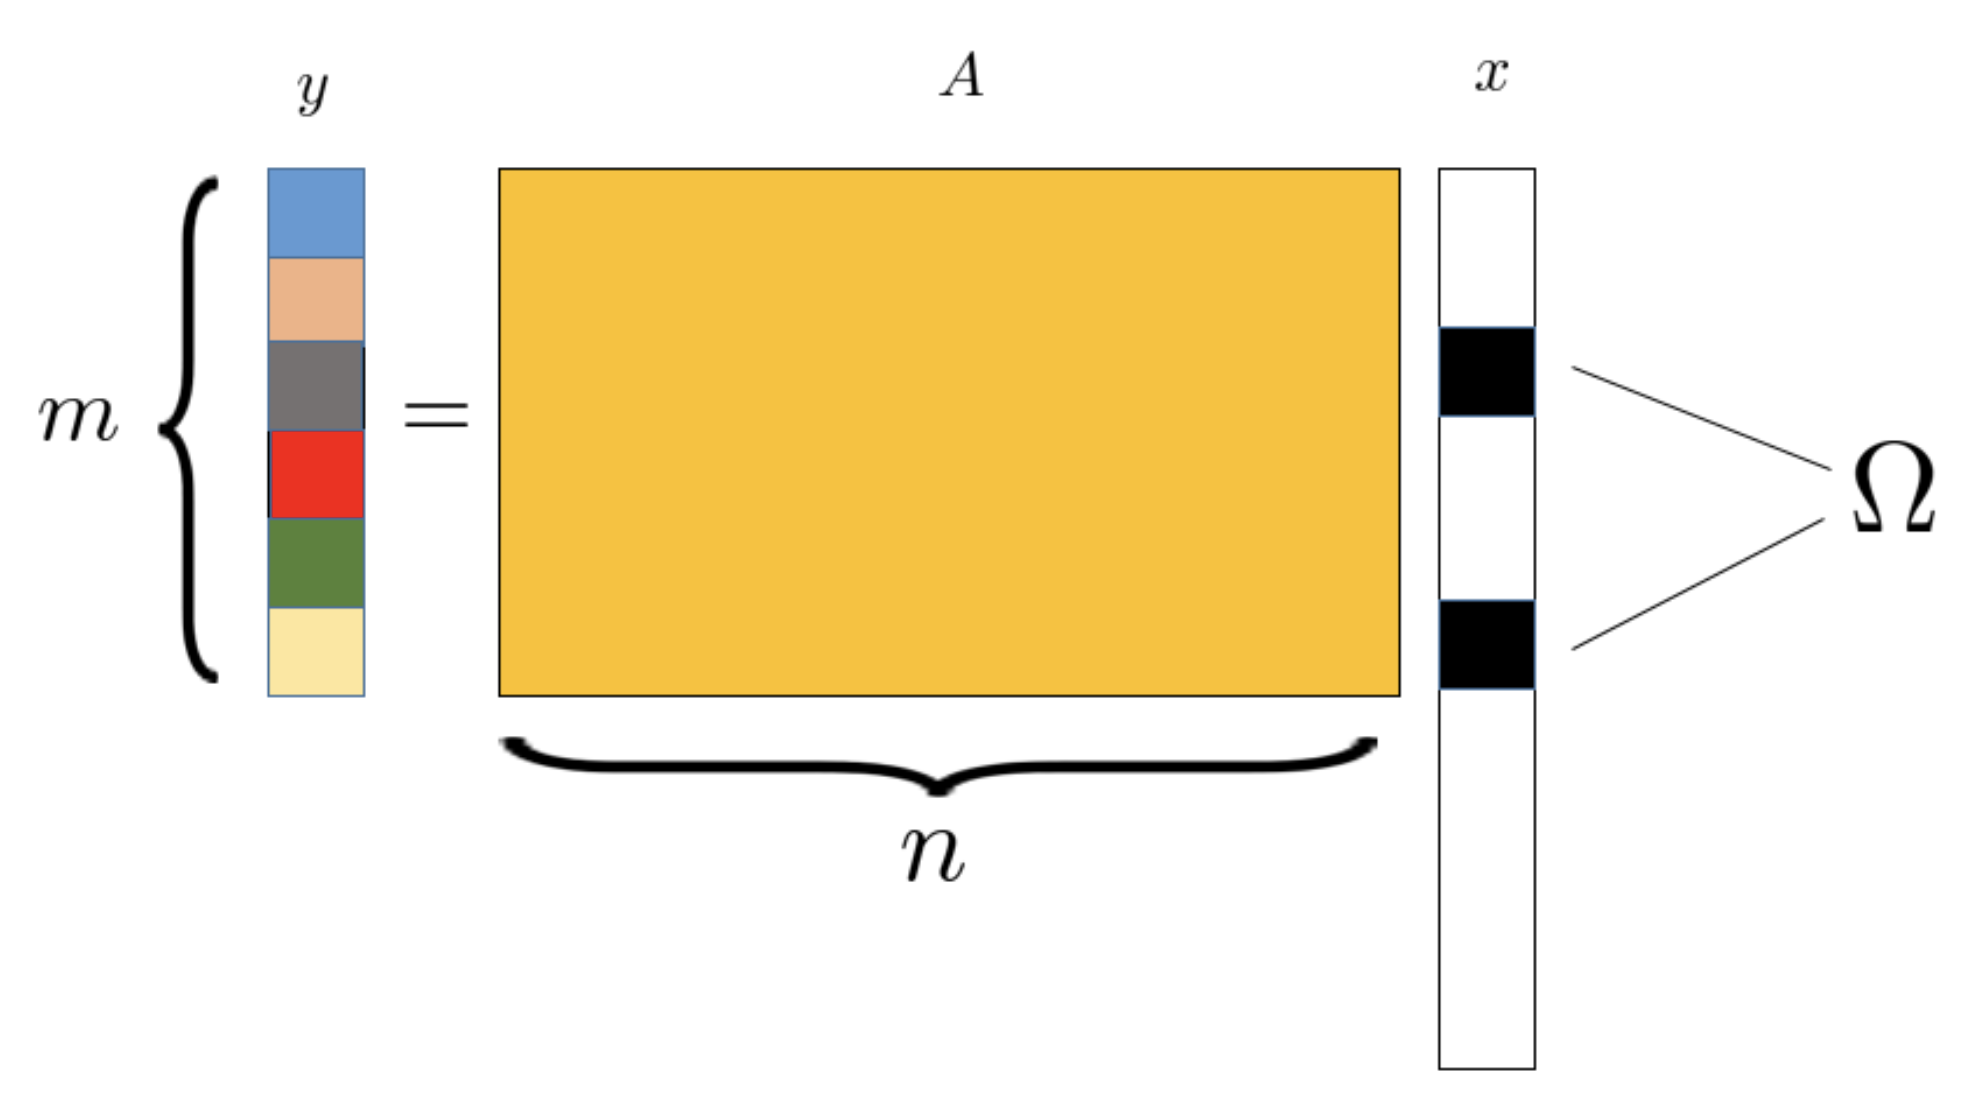
\includegraphics[scale=0.2]{MM.png}
    \caption{Measurement of sparse signal $\vec{x}$ with support set $\Omega$ of size $k$.}
    \label{}
\end{figure}\end{center}
Denote by $A_i$, $1 \leq i \leq n$ the column vectors of $A$ and let $\Omega \subset \{1,2,...,n\}$ be the support set of the vector $\vec{x}$, i.e., $\Omega = \{i : x_i \neq 0\}$. Define the reduced matrix $A_\Omega = \{A_i, i \in \Omega\}$ and the reduced vector $\vec{x}_\Omega =\{x_i, i\in \Omega\}$. Then $$\vec{y}=A \vec{x}=A_\Omega \vec{x}_\Omega $$



\subsection{Matrix Preliminaries}
The SVD decomposition of $A$ takes the form $A=U[D \mid 0] V^T$ where $U$ and $V$ are $m \times m$ and $n \times n$ unitary matrices (whose conjugate transpose equals to inverse), respectively, $\mathrm{D}=\operatorname{diag}\left(\sigma_k\right)_{k=1}^m$, and 0 is the $m \times(n-m)$ all-zero matrix. The $m$ nonnegative entries $\sigma_k, 1 \leq k \leq m$, are the singular values of $A$. The matrix A can be expanded as a sum of $m$ rank-one matrices, $\mathrm{A}=\sum_{k=1}^m \sigma_k u_k v_k^{\top}$ where $\left\{u_k\right\}$ and $\left\{v_k\right\}$ are the columns of $U$ and $V$, respectively.

The spectral norm of $A$ is
$$
\|\mathrm{A}\| \triangleq \sup _{\vec{x}:\|\vec{x}\|_2=1}\|\mathrm{A} \vec{x}\|_2
$$
and is equal to the largest singular value of $A$.

The $m \times m$ Gram matrix $\mathrm{G} \triangleq \mathrm{AA}^{\top}$ is symmetric and nonnegative definite and can be expressed as $\mathrm{G}=\mathrm{UD}^2 \mathrm{U}^{\top}$ hence its eigenvalues are given by $\lambda_k(\mathrm{G})=\sigma_k^2(\mathrm{~A}), 1 \leq k \leq m$.

\begin{definition}[Null Space]
    The \underline{null space} of $\mathrm{A}$ is $$N(\mathrm{A}) \triangleq\left\{\vec{x} \in \mathbb{R}^n: \mathrm{A} \vec{x}=0\right\}$$
    This is a subspace of $\mathbb{R}^n$, whose dimension is \underline{at most $n - m$}.
\end{definition}

\begin{definition}[Spark]
    The \underline{spark} of $A$ is the smallest number of columns of $A$ that are linearly dependent.\\
    If any set of $q$ columns of the matrix are linearly independent, $\textnormal{spark}(A)=q+1\in [2,m+1]$.
\end{definition}
The minimum value of the spark of any matrix is $2$, and is achieved by any matrix that has two identical columns.

Computing the spark of a matrix in an \underline{NP-hard problem}. In contrast, the rank of a matrix, which is the largest number of columns that are linearly independent, is easy to compute.

\subsection{Recovery of k-Sparse Signals}
\begin{lemma}
    Unique recovery of $x \in \Sigma_k$ given measurement matrix $A$ is possible $\Rightarrow$ $\Sigma_{2k} \cap N(A) = \emptyset$.
\end{lemma}
\begin{proof}
    To recover any \underline{$k$-sparse signal}, we need that $A\vec{x} \neq A\vec{x}'$ for any distinct $\vec{x},\vec{x}' \in \Sigma_k$. Hence, $\vec{x}-\vec{x}' \notin N(A)$. Since $\vec{x}-\vec{x}'$ is a $2k$-sparse signal and in fact $\Sigma_{2k} ={\vec{x}-\vec{x}' : \vec{x},\vec{x}'\in \Sigma_k}$, we need $\Sigma_{2k} \cap N(A) = \emptyset$.
\end{proof}

\begin{theorem}
    Unique recovery of $\vec{x} \in \Sigma_k$ given measurement matrix $A$ is possible $\Leftrightarrow$ $\textnormal{spark}(A)> 2k$. ($q\geq 2k$)
\end{theorem}
\begin{proof}
Eldar, Y. C., \& Kutyniok, G. (Eds.). (2012). Compressed sensing: theory and applications, Chapter 1.
\end{proof}

\subsection{Restricted Isometry Property}
\begin{definition}[Restricted Isometry Property (RIP)]
    The matrix $A$ satisfies the \underline{RIP property of order $k$} if there exists $\delta_k \in (0, 1)$ such that
    \begin{equation}
        \begin{aligned}
            (1-\delta_k)\|\vec{x}\|^2_2\leq\|A\vec{x}\|_2^2\leq (1+\delta_k)\|\vec{x}\|^2_2,\quad \forall \vec{x}\in \Sigma_k
        \end{aligned}
        \nonumber
    \end{equation}
\end{definition}
If $A$ satisfies the RIP property of order $k$, then $A$ approximately \underline{preserves the $\ell_2$ distance} between any pair $\vec{x},\vec{x}' \in \Sigma_k$. This provides a \textit{stable embedding} of $k$-sparse signals in $\mathbb{R}^m$. This property will be key to derive a recovery algorithm that is robust to noise.

\begin{claim}[Equivalent Formulation of RIP]
    Since $\vec{y}=A \vec{x}=A_\Omega \vec{x}_\Omega$, an \textbf{equivalent formulation} of the RIP is $$(1-\delta_k)\|\vec{x}_\Omega\|^2_2\leq\|A_\Omega \vec{x}_\Omega\|_2^2\leq (1+\delta_k)\|\vec{x}_\Omega\|^2_2,\quad \forall \Omega: |\Omega|=k$$
for all $\Omega$ of size $k$ and for all $\vec{x}_\Omega\in \mathbb{R}^k$.
\begin{equation}
    \begin{aligned}
        \frac{\|A_\Omega \vec{x}_\Omega\|_2^2}{\|\vec{x}_\Omega\|_2^2}-1&=\frac{\vec{x}_\Omega^T\left(A^T_\Omega A_\Omega-I_k\right)\vec{x}_\Omega}{\vec{x}_\Omega^T\vec{x}_\Omega}\in\left[-\delta_k,\delta_k\right],\quad \forall \Omega: |\Omega|=k\\
        \Rightarrow \delta_k&=\max_{\Omega:|\Omega|=k}\|A^T_\Omega A_\Omega-I_k\|
    \end{aligned}
    \nonumber
\end{equation}
\end{claim}

\begin{theorem}[Measurement Bound]
    Assume $A\in \mathbb{R}^{m\times n}$ satisfies the RIP of order $2k$ with RIP constant $\delta_{2k}\in (0,\frac{1}{2}]$. Then $$m\geq ck\ln\frac{n}{k}$$ where the constant $c=\frac{1}{2}\ln(1+\sqrt{24})\approx 0.28$.
\end{theorem}

\section{Robust Signal Recovery from Noiseless Observations}
We now consider the so-called robust CS problem: the signal $\vec{x}$ is approximately sparse, and the observations are noiseless. A reasonable attempt to recover a sparse signal would be the so-called $\ell_0$ recovery problem
$$
\min _{\vec{x} \in \mathbb{R}^n}\|\vec{x}\|_0 \quad \text { subj. to } \quad \mathrm{A} \vec{x}=\vec{y}
$$
Unfortunately this problem is highly nonconvex. Solving it essentially requires evaluating all possible support sets of $\vec{x}$, which is a combinatorial problem.

A reasonable substitute is the so-called $\ell_1$ recovery problem
$$
\min _{\vec{x} \in \mathbb{R}^n}\|\vec{x}\|_1 \quad \text { subj. to } \quad \mathrm{A} \vec{x}=\vec{y}
$$
This procedure tends to produce sparse solutions, as illustrated in the Figure: the line $y=A x$ is tangent to the $\ell_1$ ball $\|\boldsymbol{x}\|_1=$ cst at the solution $\boldsymbol{x}$, producing a 1-sparse solution.
\begin{center}\begin{figure}[htbp]
    \centering
    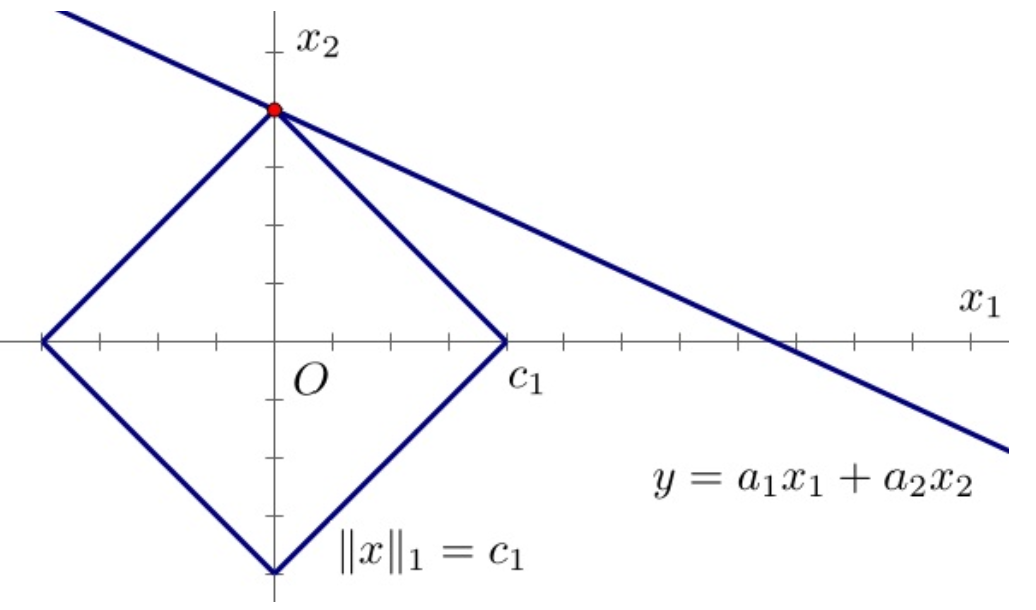
\includegraphics[scale=0.25]{l1re.png}
    \caption{$\ell_1$ recovery for $n=2$ and $m=1$}
    \label{}
\end{figure}\end{center}
The following fundamental theorem shows that the $\ell_1$ recovery procedure is remarkably good.
\begin{theorem}[$\ell_1$ recovery procedure is good]
    Assume $A$ satisfies the RIP of order $2 k$ with constant $\delta_{2 k}<\sqrt{2}-1$. $\hat{x}=\argmin_{\vec{x}\in \mathbb{R}^n: A \vec{x}=\vec{y}}\|\vec{x}\|_1$. Then
    $$
    \|\hat{x}-x\|_2 \leq \frac{c}{\sqrt{k}} e_{k,1}(x)
    $$
    and
    $$
    \|\hat{x}-x\|_1 \leq c e_{k,1}(x)
    $$
    with $c=2 \frac{1-(1-\sqrt{2}) \delta_{2 k}}{1-(1+\sqrt{2}) \delta_{2 k}}$. $e_{k,1}(x)\triangleq \min_{\hat{x}\in \Sigma_k}\|x-\hat{x}\|_1$ is the \underline{$\ell_1$ approximation error} of $x$ in $\Sigma_k$.
\end{theorem}
\begin{proof}
    Based on the triangle inequality and the inequality $\frac{\|u\|_1}{\sqrt{k}} \leq\|u\|_2 \leq \sqrt{k}\|u\|_{\infty}$ for all $u \in \Sigma_k$.
\end{proof}

\begin{corollary}
    If $x \in \Sigma_k$ then $\hat{x}=x$ (exact recovery).
\end{corollary}
If $x \notin \Sigma_k$ then the quality of the reconstruction is nearly as good as if an \textit{oracle} gave us the location of the $k$ largest absolute components and we measured those directly. (The oracle produces $\hat{x}=H_k(x)$, achieving $e_{k, p}(x)$ for all $p \geq 1$.)

Since $\delta_{2 k}<\sqrt{2}-1<\frac{1}{2}$, the measurement bound $m\geq ck\ln\frac{n}{k}$ applies, and we need as few as $m=O\left(k \ln \frac{n}{k}\right)$ measurements to satisfy the conditions of the theorem.

\section{Robust Signal Recovery from Noisy Observations}
\subsection{Bounded Noise}
We consider observations corrupted by bounded noise: $y=\mathrm{A} x+z$ where $\|z\|_2 \leq \epsilon$. We study the $\ell_1$ recovery problem
$$
\min _{x \in \mathbb{R}^n}\|x\|_1 \quad \text { subj. to } \quad\|\mathrm{A} x-y\|_2 \leq \epsilon
$$
which is closely related to the Lasso problem and can be solved using the algorithms introduced in the previous chapter.
\begin{theorem}
    Assume A satisfies the RIP of order $2 k$ with constant $\delta_{2 k}<\sqrt{2}-1$. Then
    $$
    \|\hat{x}-x\|_2 \leq \frac{c_0}{\sqrt{k}} e_{1, k}(x)+c_1 \epsilon
    $$
    with constants
    $$
    c_0=2 \frac{1-(1-\sqrt{2}) \delta_{2 k}}{1-(1+\sqrt{2}) \delta_{2 k}}, \quad \text { and } \quad c_1=4 \frac{\sqrt{1+\delta_{2 k}}}{1-(1+\sqrt{2}) \delta_{2 k}} .
    $$
\end{theorem}
For $\delta_{2 k}=\frac{1}{4}$ the theorem holds with $c_0 \leq 5.5$ and $c_1 \leq 6$. For $\epsilon=0$, the result coincides with that given in the previous section (noise-free case).







\end{document}